\documentclass{amsbook} % default font size is 10pt
\usepackage{latexsym}
\usepackage{amsfonts}
\usepackage[bbgreekl]{mathbbol}
\usepackage{amssymb}
\usepackage{amsmath}
\usepackage{amscd}
\usepackage{longtable}
\usepackage{array}
\usepackage{graphicx}
\usepackage{eucal}
\usepackage{multicol}
\usepackage[refpage, notintoc]{nomencl}
% \renewcommand{\nomname}{}
\renewcommand*{\pagedeclaration}[1]{\,\,\,\hyperpage{#1}}
\makenomenclature
\makeindex
\usepackage{etoolbox}
\renewcommand\nomgroup[1]{%
  \item[\bfseries
  \ifstrequal{#1}{C}{\addcontentsline{toc}{section}{Catalogue of Categories}  \rule[2pt]{0.45\linewidth}{1pt} Catalogue of Categories  \rule[2pt]{0.45\linewidth}{1pt}}{%
  \ifstrequal{#1}{N}{\addcontentsline{toc}{section}{Glossary of Notation} \rule[2pt]{0.45\linewidth}{1pt} Glossary of Notation  \rule[2pt]{0.45\linewidth}{1pt}}{}}%
]}
\usepackage[all]{xy}
\usepackage{tikz}
\usetikzlibrary{decorations.markings,decorations.pathmorphing}
\usetikzlibrary{arrows}
\usepackage{tikz-cd}
%\tikzset{/tikz/commutative diagrams/arrow style=math font} % matching arrowheads
\tikzset{/tikz/commutative diagrams/arrow style=tikz,>=stealth} %almost matching arrowheads; look better in pdf
\tikzset{mm/.style={execute at begin node=$\displaystyle, execute at end node=$}}
\tikzset{tikzob/.style={commutative diagrams/every diagram, every cell}}
\tikzset{tikzar/.style={commutative diagrams/.cd, every arrow, every label, font={\small}}}
\tikzset{tikzsquiggle/.style={decorate, decoration={
    snake,
    segment length=8pt,
    amplitude=.9pt,post=lineto,
    post length=2pt}}}
\tikzset{cross line/.style={preaction={draw=white, -, line width=6pt}}}
\usepackage{pdfsync}
\usepackage{relsize}
\usepackage{pdfsync}
\usepackage[unicode=true, pdfusetitle,
 bookmarks=true,bookmarksnumbered=false,
 breaklinks=false,
 backref=false,
 colorlinks=true,
 %linkcolor=blue!70!black,
 citecolor=black,
 urlcolor=blue!78!red,
 final
]{hyperref}
\usepackage[capitalise]{cleveref}
\newcommand{\fref}{\cref}
\newcommand{\Fref}{\Cref}
\newcommand{\prettyref}{\cref}
\newcommand{\newrefformat}[2]{}
\newcommand{\cn}{\colon}
\newcommand{\bs}{\boldsymbol}
\newcommand{\mb}{\mathbf}
\renewcommand{\dot}{\centerdot}
\newcommand{\R}{\mathbb{R}}
\newcommand{\ZZ}{\mathbb{Z}}
\newcommand{\N}{\mathbb{N}}
\newcommand{\m}[1]{\mathcal{#1}}
\newcommand{\id}{\textrm{id}}
\newcommand{\un}{\underline}
%\usepackage{natbib}
\renewcommand{\SS}{\mathcal{S}}
\newcommand{\colim}{\textrm{colim }}
\newcommand{\und}[1]{\ensuremath{\underline{#1}}}
\newcommand{\f}[1]{\ensuremath{\mathcal{#1}}}
\newcommand{\g}[1]{\ensuremath{\mathbb{#1}}}
\newcommand{\Cat}{\ensuremath{\textrm{Cat}}}
\newcommand{\cd}[2][]{\vcenter{\hbox{\xymatrix#1{#2}}}}
\newcommand{\Set}{\ensuremath{\textrm{Set}}}
\newcommand{\twocat}{\ensuremath{\textrm{2-Cat}}}
\newcommand{\Icon}{\ensuremath{\textrm{Icon}}}
\newcommand{\ML}{\mathbf{\Lambda}}
\newcommand{\LL}{\Lambda}
%\newcommand{\to}{\rightarrow}
\def\srarrow{\relbar\joinrel\mapstochar\joinrel\rightarrow}
%\newcommand{\id}{\ensuremath{\textnormal{id}}\xspace}
%\pdfshift
\newcommand{\quotient}[2]{ \raisebox{0.5\height}{$#1$} \mkern-5mu\diagup\mkern-4mu \raisebox{-0.5\height}{$#2$} }
\newcommand{\bigquotient}[2]{ \raisebox{0.75\height}{$#1$} \mkern-12mu\scalebox{2}{$\diagup$}\mkern-10mu \raisebox{-0.5\height}{$#2$} }
\newcommand{\pullback}{\mathbin{\text{\rotatebox{45}{$\mathlarger{\mathlarger{\mathlarger{\mathlarger{\llcorner}}}}$}}}}
\newcommand{\pushout}{\mathbin{\text{\rotatebox{225}{$\mathlarger{\mathlarger{\mathlarger{\mathlarger{\llcorner}}}}$}}}}
\newcommand{\downsim}{\rotatebox{90}{$\sim$}}
\newcommand{\EL}{E\Lambda}
\newcommand{\ELn}{E\Lambda(\underline{n})}
\newcommand{\ELnn}{E\Lambda(\underline{2n})}
\newcommand{\ELnnnn}{E\Lambda(\underline{4n})}
\newcommand{\ob}{\textrm{Ob}}
\newcommand{\lmc}{\Lambda\mbox{-}\mb{MonCat}}
\newcommand{\sets}{\Set}
\newcommand{\mon}{\ensuremath{\mb{Mon}}}
\newcommand{\cmon}{\ensuremath{\mb{CommMon}}}
\newcommand{\moncat}{\ensuremath{\mb{MonCat}}}
\newcommand{\cat}{\ensuremath{\mb{Cat}}}
\newcommand{\epz}{\varepsilon}
\newcommand{\Alg}{\mbox{-}\mb{Alg}}
\newcolumntype{L}{>{$}l<{$}}
\newcolumntype{C}{>{$}c<{$}}
\newcolumntype{R}{>{$}r<{$}}

\crefname{lem}{Lemma}{Lemmas}
\crefname{thm}{Theorem}{Theorems}
\crefname{Defi}{Definition}{Definitions}
\crefname{nota}{Notation}{Notations}
\crefname{construction}{Construction}{Constructions}
\crefname{prop}{Proposition}{Propositions}
\crefname{rem}{Remark}{Remarks}
\crefname{cor}{Corollary}{Corollaries}
\crefname{scholium}{Scholium}{Scholia}
\crefname{figure}{Figure}{Figures}
\crefname{equation}{Equation}{Equations}
\crefname{eq}{Equation}{Equations}
\crefname{eqn}{Equation}{Equations}

\newenvironment{eq}{\begin{equation}}{\end{equation}}
\newenvironment{eqn}{\begin{equation}}{\end{equation}}
\newenvironment{eq*}{\begin{equation*}}{\end{equation*}}
\newenvironment{eqn*}{\begin{equation*}}{\end{equation*}}
\tikzset{->-/.style={decoration={markings,mark=at position #1 with {\arrow{>}}},postaction={decorate}}} 

\pgfdeclarelayer{bg}
\pgfsetlayers{bg,main}

\numberwithin{section}{chapter}


\begin{document}
\newtheorem{thm}{Theorem}[section]
\newtheorem{prop}[thm]{Proposition}
\newtheorem{lem}[thm]{Lemma}
\newtheorem{cor}[thm]{Corollary}

\newtheoremstyle{example}{\topsep}{\topsep}%
     {}%         Body font
     {}%         Indent amount (empty = no indent, \parindent = para indent)
     {\bfseries}% Thm head font
     {.}%        Punctuation after thm head
     {2pt}%     Space after thm head (\newline = linebreak)
     {\thmname{#1}\thmnumber{ #2}\thmnote{ #3}}%         Thm head spec
		
		

   \theoremstyle{example}
	\newtheorem{conv}[thm]{Conventions}
   \newtheorem{nota}[thm]{Notation}
   \newtheorem{example}[thm]{Example}
	\newtheorem{Defi}[thm]{Definition}
   \newtheorem{rem}[thm]{Remark}

   \title[Operads]{Operads and equivariance}

\author{Alexander S. Corner}
\address{}
\email{alex.corner@shu.ac.uk}
\author{Nick Gurski}
\address{}
\email{nick.gurski@case.edu}
\author{Edward Prior}
\address{}
\email{}
\keywords{}
\subjclass{}

\maketitle

\tableofcontents


\chapter{Introduction}








\chapter{Invertible objects}


The goal of this chapter will be to show that we can reconstruct all of the morphisms of $L_n$ from the abelian group $\mathrm{M}(L_n)^{\mathrm{gp, ab}}$, and therefore that we can actually use the adjunction from \cref{Moradj} to help find a description of the free $E\Lambda$-algebra on $n$ invertible objects. 

The first step towards this goal will involve splitting $\mathrm{Mor}(L_n)$ up as the product of two other monoids. The first of these will encode all of the possible combinations of source and target data for morphisms in $L_n$, while the second will just be the endomorphisms of the unit object, $L_n(I, I)$. 
Once we have done this, we can then use the fact that $L_n(I, I)$ is always an abelian group to rewrite $\mathrm{Mor}(L_n)$ in terms of its abelian group completion, $\mathrm{Mor}(L_n)^{\mathrm{gp, ab}}$. This is not quite the same thing as $\mathrm{M}(L_n)^{\mathrm{gp, ab}}$, but they are close enough that we can find a simple equation linking the two, which will in turn allow us to frame the former in terms of the quotient of $\mathrm{M}(\ELnn)^{\mathrm{gp, ab}}$ we described last chapter. All together, this will constitute an expression for $\mathrm{Mor}(L_n)$ that is built up of pieces which we know how to calculate.

\section{Introduction to invertibility}

Our main focus will be on invertible objects, although not in the usual sense.
\begin{Defi}
Let $(M, \otimes, I)$ be a monoidal category. An object $m \in M$ is \emph{invertible}\index{object!invertible} if there exists another object $m^{-1}$ such that $m \otimes m^{-1} = I$ and $m^{-1} \otimes m = I$.

\end{Defi}

Most authors give the following as the definition of an invertible object, what we call weakly invertible.
\begin{Defi}
Let $(M, \otimes, I)$ be a monoidal category. An object $m \in M$ is \emph{weakly invertible}\index{object!weakly invertible} if there exists another object $m^{*}$ such that $m \otimes m^{*} \cong I$ and $m^{*} \otimes m \cong I$.

\end{Defi}

We will later derive results about weakly invertible objects from those about invertible ones using standard 2-monadic techniques.



\begin{Defi} Given an $E\Lambda$-algebra $X$, we will denote by $X_{\mathrm{inv}}$\nomenclature[N]{$X_{\mathrm{inv}}$}{the sub-$E\Lambda$-algebra of $X$ of objects invertible under tensor product}\index{algebra!of weakly invertible objects} the sub-$E\Lambda$-algebra of $X$ containing all objects which are invertible under tensor product, and all of the isomorphisms between them. \end{Defi} 

First note that this is indeed a well-defined $E\Lambda$-algebra since the tensor product of invertible objects is again invertible, the tensor product of isomorphisms is again an isomorphism, and all of the morphisms giving the group actions are isomorphisms. The following proposition is then obvious.


\begin{prop} \label{invprop} The assignment $X \mapsto X_{\mathrm{inv}}$ can be extended to a 2-functor $(\_)_{\mathrm{inv}}: E\Lambda\mbox{-}\mb{Alg}_S \to E\Lambda\mbox{-}\mb{Alg}_S$.
\end{prop}


\begin{prop} \label{invadj} The 2-functor $(\_)_{\mathrm{inv}}: E\Lambda\mbox{-}\mb{Alg}_S \to E\Lambda\mbox{-}\mb{Alg}_S$ has a left adjoint, $L: E\Lambda\mbox{-}\mb{Alg}_S \to E\Lambda\mbox{-}\mb{Alg}_S$.
\end{prop}
\begin{proof} Since we already know that $E\Lambda\mbox{-}\mb{Alg}_S$ is locally finitely presentable, the conditions for \cref{aftlfp} amount to showing that $(\_)_{\mathrm{inv}}$ preserves both limits and filtered colimits.
\begin{itemize}
\item Given an indexed collection of $E\Lambda$-algebras $X_i$, the $E\Lambda$-action of their product $\prod X_i$ is defined componentwise. In particular, this means that the tensor product of two objects in $\prod X_i$ is just the collection of the tensor products of their components in each of the $X_i$. An invertible object in $\prod X_i$ is thus simply a family of invertible objects from the $X_i$, so $(\prod X_i)_{\mathrm{inv}} = \prod (X_i)_{\mathrm{inv}}$.
\item Given maps of $E\Lambda$-algebras $F: X \to Z$, $G : Y \to Z$, the $E\Lambda$-action of their pullback $X \times_Z Y$ is also defined component-wise. It follows that an invertible object in $X \times_Z Y$ is just a pair of invertible objects $(x, y)$ from $X$ and $Y$, such that $F(x) = G(y)$. But this is the same as asking for a pair of objects $(x, y)$ from $X_{\mathrm{inv}}$ and $Y_{\mathrm{inv}}$ such that $F_{\mathrm{inv}}(x) = G_{\mathrm{inv}}(y)$, and hence $(X \times_Z Y)_{\mathrm{inv}} = X_{\mathrm{inv}} \times_{Z_{\mathrm{inv}}} Y_{\mathrm{inv}}$.
\item Given a filtered diagram $D$ of $E\Lambda$-algebras, the $E\Lambda$-action of its colimit $\mathrm{colim}(D)$ is defined in the following way: use filteredness to find an algebra which contains (representatives of the classes of) all the things you want to act on, then apply the action of that algebra. In the case of tensor products this means that $[x]\otimes[y] = [x \otimes y]$, and thus an invertible object in $\mathrm{colim}(D)$ is just (the class of) an invertible object in one of the algebras of $D$. In other words, $\mathrm{colim}(D)_{\mathrm{inv}} = \mathrm{colim}(D_{\mathrm{inv}})$.
\end{itemize}
Preservation of products and pullbacks give preservation of limits, and preservation of limits and filtered colimits together give the result.
\end{proof}



\begin{Defi}
Let $L_n = L\Big(E\Lambda(\underline{n}) \Big)$\nomenclature[C]{$L_n$}{the free $\ML$-monoidal category on $n$ invertible objects}\index{monoidal category!$\ML$-monoidal!free}, where $\underline{n} = \{x_1, \ldots, x_n \}$ is a set with $n$ elements.
\end{Defi}

\begin{thm} The algebra $L_n$ is the free $\ML$-monoidal category on $n$ invertible objects:  for any other $E\Lambda$-algebra $X$, we have an isomorphism of categories
\[ E\Lambda\mbox{-}\mb{Alg}_S(L_n, X) \quad \cong \quad (X_{\mathrm{inv}})^n, \]
2-natural in $X$.
\end{thm}
\begin{proof}
We have the following 2-natural isomorphisms from the adjunctions for $L$ and the free $\ML$-monoidal category monad.
\[\begin{array}{rll}
		 E\Lambda\mbox{-}\mb{Alg}_S( L\Big(E\Lambda(\underline{n}) \Big), X) & \cong  & E\Lambda\mbox{-}\mb{Alg}_S( E\Lambda(\underline{n}), X_{inv}) \\
		& \cong & \cat( \underline{n}, X_{inv}) \\
		& \cong & X_{inv}^n
\end{array}
 \]


\end{proof}

\begin{prop} \label{linveql} For any $E\Lambda$-algebra $X$, we have $L(X)_{\mathrm{inv}} = L(X)$.
\end{prop}
\begin{proof}
Let $j: X_{inv} \to X$ denote the obvious inclusion functor. By construction, we have an equality of functors $(\_)_{\mathrm{inv}} \circ (\_)_{\mathrm{inv}} = (\_)_{\mathrm{inv}}$ and moreover $j_{inv}: (X_{inv})_{inv} \to X_{inv}$ is the identity for every $X$. Since $E\Lambda\mbox{-}\mb{Alg}_S(LX , Y)\cong E\Lambda\mbox{-}\mb{Alg}_S(X, Y_{\mathrm{inv}})$ is natural in $Y$, we have a commutative square
\begin{center}
    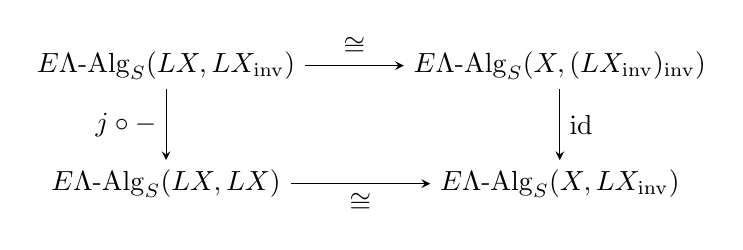
\begin{tikzpicture}[x=50mm,y=15mm]
		\node (a) at (0,0) {$E\Lambda\mbox{-}\mathrm{Alg}_S(LX , LX_{\mathrm{inv}})$};
		\node (b) at (1,0) {$E\Lambda\mbox{-}\mathrm{Alg}_S(X, (LX_{\mathrm{inv}})_{\mathrm{inv}})$};
		\node (c) at (0,-1) {$ E\Lambda\mbox{-}\mathrm{Alg}_S(LX , LX)$};
		\node (d) at (1,-1) {$E\Lambda\mbox{-}\mathrm{Alg}_S(X, LX_{\mathrm{inv}})$};
			\draw [->] (a) to node [above] {$\cong$} (b);
			\draw [->] (b) to node [right] {$\mathrm{id}$} (d);
			\draw [->] (a) to node [left] {$j \circ -$} (c);
			\draw [->] (c) to node [below] {$\cong$} (d);
    \end{tikzpicture}
    \end{center}
in which the identity on the right is really $j_{inv} \circ -$. Thus composition with $j$ is an isomorphism in this case, so the identity map on $LX$ factors as $j \circ g$ for some $g: LX \to (LX)_{inv}$. Since $j$ is an inclusion, this factorization forces it to be the identity.


\end{proof}


\begin{cor} \label{epi} The component of the unit of the adjunction $L \dashv (-)_{inv}$ at $E\Lambda(\underline{n})$,  $\eta_{E\Lambda(\underline{n})}: E\Lambda(\underline{n}) \to (L_n)_{inv}$, is an epimorphism in $E\Lambda\mbox{-}\mathrm{Alg}_S$.
\end{cor}
\begin{proof}

By \cref{linveql}, we first have that $(L_n)_{inv} = L_n$. Let $F,G: L_n \to X$ be a pair of algebra maps for which $F \eta = G \eta$. Thus the algebra maps $E\Lambda(\underline{n}) \to X_{inv}$ corresponding to $F, G$ are equal, so $F,G$ are equal.




\end{proof}


QQQ Need to explain that the goal is to understand some group actions


\section{Adjunctions involving monoidal categories}

This section will study three different adjunctions between $\ML$-monoidal categories\index{monoidal category!$\ML$-monoidal} on the one hand and categories such as that of monoids or commutative monoids on the other hand. Two of these adjunctions are purely formal, and are induced by adjunctions between categories and sets, while the third requires a direct proof. We then investigate some simple consequences of these adjunctions for $\ML$-monoidal categories of the form $L(E\Lambda S)$ for a set $S$.

\begin{prop}\label{Ob-E_adj}
The functor $\ob$ from categories to sets, taking the set of objects, is left adjoint to the functor $E$ of \cref{Defi:e_b} QQQ. This adjunction is monoidal, hence induces an adjunction $\ob \dashv E$ between $\lmc$ and $\mon$\nomenclature[C]{$\mon$}{of monoids and monoid homomorphisms}.
\end{prop}
\begin{proof}
This is a straightforward application of \cref{...}; the only thing to note is that $\ob(\EL) = \Lambda$ as a $\ML$-operad.

\end{proof}

\begin{Defi}
Let $\ML$ be an action operad. Let $T_{\ML}$\nomenclature[N]{$T_{\ML}$}{the terminal $\ML$-operad} denote the terminal $\ML$-operad in sets, which is a singleton set in each dimension with the unique action of $\Lambda_n$.
\end{Defi}

\begin{lem}
The category of algebras for $T_{\ML}$ is either the category of monoids, when $\ML$ is not crossed, or the category of commutative monoids, when $\ML$ is crossed.
\end{lem}
\begin{proof}
In the case that $\ML$ is not crossed, $\Lambda(n)$ acts on $X^n$ trivially so the free $T_{\ML}$-algebra monad coincides with the free monoid monad. When $\ML$ is crossed, $\Lambda(n)$ acts on $X^n$ via the surjection to $\Sigma_n$ so the free $T_{\ML}$-algebra monad coincides with the free commutative monoid monad.
\end{proof}

\begin{nota}
We write $D$ for the discrete category functor $\sets \to \cat$.
\end{nota}

\begin{prop}\label{pi0-D_adj}
The functor $\pi_0$ from categories to sets, taking the set of path components, is left adjoint to  $D$. This adjunction is monoidal, hence induces an adjunction between $\lmc$ and $T_{\ML}\mbox{-}\textrm{Alg}$.
\end{prop}
\begin{proof}
This is now a simple application of \cref{monoidaladj_cor}, where we now only note that the unit $1 \Rightarrow \pi_0 \circ D$ is the identity transformation.
\end{proof}



\begin{Defi} For a monoid $M$, we write $M^{\mathrm{gp}}$ for its \emph{group completion}\index{group completion}, the universal group with a homomorphism $M \to M^{gp}$.  We write the functor $M \mapsto M^{gp}$ as $gp$.
\end{Defi}

\begin{rem}
The category of groups is a reflective subcategory of the category of monoids, and $gp$ is the reflection.
\end{rem}

\begin{prop}\label{oblel_fg}
The functor $\ob \circ L \circ \EL: \sets \to \mon$ is naturally isomorphic to the composite of the free group functor and the inclusion of groups into monoids.
\end{prop}
\begin{proof}
Using that the objects of $\EL(M)_{inv}$ for a monoid $M$ are the same as the objects of $\EL(M^{\times})$, where $M^{\times}$ is the subgroup of invertible elements of $M$, we see that both of these functors are left adjoints to the functor $M \mapsto M^{\times}$.
\end{proof}
There are several different ways to actually calculate the group completion of a monoid. One is to use that fact that $M^{\mathrm{gp}}$ is the group whose group presentation is the same as the monoid presentation of $M$. That is, if $M$ is the quotient of the free monoid on generators $\mathcal{G}$ by the relations $\mathcal{R}$, then $M^{\mathrm{gp}}$ is the quotient of the free \emph{group} on generators $\mathcal{G}$ by relations $\mathcal{R}$. This makes finding the completion of free monoids particularly simple.

\begin{nota}
We write $M^{*n}$\nomenclature[N]{$M^{*n}$}{the coproduct of $n$ copies of the monoid $M$} for the coproduct of $n$ copies of the monoid $M$. We use the same notation for groups, although the $n$-fold coproduct of a group is different when considered as a monoid than as a group; it should be clear from context which we intend.
\end{nota}

\begin{cor}\label{Zobj}
The object monoid of $L_n$ is $\mathbb{Z}^{*n}$\nomenclature[N]{$\mathbb{Z}$}{the set of integers}, the group completion of the object monoid of $\ELn$. The restriction of $\eta$ on objects, $\mathrm{Ob}(\eta)$, is then the obvious inclusion $\mathbb{N}^{*n} \hookrightarrow \mathbb{Z}^{*n}$.
\end{cor}





The core of \cref{Zobj} --- that $\mathrm{Ob}(L_n)$ is the group completion of $\mathrm{Ob}(\ELn)$ --- makes concrete the sense in which the functor $L$ represents `freely adding inverses' to objects. Extending this same logic to connected components as well, it would seem reasonable to expect that $\pi_0(L_n)$ is also the group completion of $\pi_0(\ELn)$. This is indeed the case, and the proof proceeds in a way completely analogous to \cref{Zobj}. 




\begin{prop}\label{pilel_gppiel}
The functor $\pi_0 \circ L: \lmc \to T_{\ML}\mbox{-}\mb{Alg}$ is naturally isomorphic to the functor $\textrm{gp} \circ \pi_0$.
\end{prop}
\begin{proof}
The proof is the same style as above, with both functors being  left adjoints of the functor $M \mapsto (DM)_{inv} = D(M^{\times})$.
\end{proof}
\begin{cor}\label{Zconcomp} The connected components of $L_n$ are the group completion of the connected components of $\ELn$. Also, the restriction of $\eta$ onto connected components, $\pi_0(\eta)$, is the canonical map $\pi_0(\ELn) \to \pi_0(\ELn)^{\mathrm{gp}}$ associated with that group completion.
\end{cor}


We summarize these results below.
\begin{cor}\label{crossconcomp} If $G$ is a crossed action operad\index{action operad!crossed} then
\begin{itemize} 
\item the connected components of $L_n$ are the monoid $\mathbb{Z}^n$,
\item the restriction of $\eta$ to components is the obvious inclusion $\mathbb{N}^n \hookrightarrow \mathbb{Z}^n$, and
\item the assignment of objects to their component is given by the quotient map of abelianization $\mathrm{ab}: \mathbb{Z}^{\ast n} \to \mathbb{Z}^n$.
\end{itemize}
If instead $G$ is non-crossed, then
\begin{itemize} \itemsep0em
\item the connected components of $L_n$ are the monoid $\mathbb{Z}^{\ast n}$,
\item the restriction of $\eta$ to components is the obvious inclusion $\mathbb{N}^{\ast n} \hookrightarrow \mathbb{Z}^{\ast n}$, and
\item the assignment of objects to their component is $\mathrm{id}_{\mathbb{Z}^{\ast n}}$.
\end{itemize}
\end{cor}

We now turn to our third adjunction, which is of a less formal nature than the first two. We begin by showing that composition along invertible objects in $X$ can always be restated in terms of the tensor product.

\begin{lem} \label{tenscomp} Let $f: x \to y$ and $f': y \to z$ be morphisms in a strict monoidal category, and assume $y$ is an invertible object with inverse $y^{-1}$. Then
\[ f' \circ f \quad = \quad f' \otimes \mathrm{id}_{y^{-1}} \otimes f \]
\end{lem}
\begin{proof}
By the interchange law for monoidal categories,
\[\begin{array}{rll} 
			f' \circ f & = & (f' \otimes \mathrm{id}_I) \circ (\mathrm{id}_I \otimes f) \\
			& = & (f' \otimes \mathrm{id}_{y^{-1}} \otimes \mathrm{id}_y) \circ (\mathrm{id}_y \otimes \mathrm{id}_{y^{-1}} \otimes f) \\
			& = & (f' \circ \mathrm{id}_y) \otimes (\mathrm{id}_{y^{-1}} \circ \mathrm{id}_{y^{-1}}) \otimes (\mathrm{id}_y \circ f) \\
			& = & f' \otimes \mathrm{id}_{y^{-1}} \otimes f .
		\end{array}
\]
\end{proof} 

Thus in cases where every object of $X$ is invertible, the monoidal structure together with knowledge of each morphism's source and target will be enough to determine $X$ uniquely. Since all objects in $L_n$ are invertible, this means that we could choose to ignore composition of elements of $\mathrm{Mor}(L_n)$ QQQ this should have had a notation environment a long time ago QQQ for the time being, and focus on its status as a monoid under tensor product.



\begin{Defi} Let $\mathrm{M} : \moncat \to \mon$ be the functor which sends a monoidal category $X$ to the quotient of its monoid of morphisms\index{monoidal category!monoid of morphisms} by the relation that sets $\otimes = \circ$. :
\[ \mathrm{M}X \quad = \quad \bigquotient{\mathrm{Mor}(X)}{f' \circ f \sim f' \otimes f}.\]
If $F:X \to Y$ is a strict monoidal functor, then $MF$ is the monoid homomorphism sending the class of a morphism $g$ to the class of $Fg$; the reader will easily check this is well-defined. We will call $\mathrm{M}X$ the \emph{collapsed} morphisms of $X$.



\end{Defi}

\begin{nota}
If $f$ is a morphism in $X$, we write its class in $\mathrm{M}X$ as $\mathrm{M}f$, and we write the single operation $\otimes$ rather than $\circ$. Note that the class $\mathrm{M}(f') \otimes \mathrm{M}(f)$ always contains $f' \otimes f$, but will only contain $f' \circ f$ if this latter morphism exists.
\end{nota}


Now we need a candidate for the right adjoint to the functor $\mathrm{M}$.

\begin{Defi} 
Let $B: \mon \to \cat$ denote the functor sending a monoid $M$ to the one-object category whose single hom-set consists of the elements of $M$, with composition and identity being given by multiplication and the unit of $M$, respectively. We also denote by $B$ the functor $\cmon \to \moncat$\nomenclature[C]{$\cmon$}{of commutative monoids and monoid homomorphisms} the functor sending a commutative monoid $A$ to the same category $BA$, now equipped with the monoidal structure which is trivial on the single object and $a \otimes b = a \circ b = ab$ on morphisms (writing the monoid operation in $A$ as concatenation here).
\end{Defi}




Note that for any monoidal category $M$, the monoid $M(I,I)$ is always commutative by the Eckmann-Hilton argument \cite{eh, cg-periodic2}, hence the requirement of commutativity to lift $B$ to a functor into monoidal categories.




\begin{Defi} For a monoid $M$, we write $M^{\mathrm{ab}}$ for its \emph{abelianization}\index{abelianization}, the universal commutative monoid with a homomorphism $M \to M^{ab}$.  We write the functor $M \mapsto M^{ab}$ as $ab$. We use the same notation for groups as well.
\end{Defi}

\begin{rem}
The categories of commutative monoids, resp. abelian groups, are reflective subcategories of the categories of monoids, resp. groups, and $ab$ is the reflection.
\end{rem}


\begin{prop}\label{Moradj} $\mathrm{B}: \cmon \to \moncat$ is a right adjoint to the functor $\mathrm{M}(\, - \,)^{\mathrm{ab}} : \moncat \to \cmon$.
\end{prop}
\begin{proof}
For a commutative monoid $A$, it is clear that $M(BA)^{ab} = A$, so we can define the counit to be the identity. For a monoidal category $X$, define $X \to B(MX^{ab})$ by sending every object of $X$ to the unique object, and by sending the morphism $f$ to the morphism given by the equivalence class of $f$. This is clearly natural in strict monoidal functors $X \to Y$, and the triangle identities make for a straightforward calculation.

\end{proof}

\cref{Moradj} seems at first glance very similar to \cref{Obadj,concompadj}. However, our goal was to discover the relationship between the morphisms of $\ELn$ and $L_n$, paralleling what we did in \cref{Zobj,Zconcomp}, and in that regard $\mathrm{M}$ falls short in two very important ways. 

\begin{enumerate}
\item Our goal was to have an adjunction involving $\lmc$, not $\moncat$, since we want to apply it to strict $\ML$-monoidal functors instead of arbitrary strict monoidal functors. 
\item Even if we do find a way to use this adjunction to extract information about $L_n$, it will not be the monoid $\mathrm{Mor}(L_n)$ we were originally after, only a strange abelianized version where tensor product and composition coincide.  
\end{enumerate} 

Unfortunately, this adjunction seems to be the best that we can do. 
\begin{prop}
The functor $B:\cmon \to \moncat$ lifts to a functor $B:\cmon \to \lmc$. This functor $B$ has a left adjoint $M':\lmc \to \cmon$, but both functors
\[
M' \circ \EL, \, M' \circ L \circ \EL : \sets \to \cmon
\]
are isomorphic to the functor sending every set to the trivial commutative monoid.
\end{prop}
\begin{proof}
To lift $B$ to $\lmc$, we need only assign the trivial action of each $\Lambda_n$. The existence of $M'$ is guaranteed by the adjoint functor theorem for locally finitely presentable categories since $B$ clearly preserves limits and filtered colimits.  For a set $S$ and commutative monoid $A$, monoid homomorphisms $M' \circ \EL(S) \to A$ are in bijection with strict $\ML$-monoidal functors $\EL(S) \to BA$ which are themselves in bijection with functions $S \to \ob(BA) = *$, so there is a unique such monoid homomorphism, and $M' \circ \EL(S) \cong 0$ as commutative monoids. The same proof works for $M' \circ L \circ \EL$ after we note that $(BA)_{inv} = BA$.
\end{proof}





 We will eventually prove that the morphisms of $L_n$ actually form a group under tensor product \cref{??}, so instead of working directly with the functor $\mathrm{M}(\, - \,)^{\mathrm{ab}}: \moncat \to \cmon$, we will focus on its composite with the group completion functor, $gp : \cmon \to \mathrm{Ab}$. We end with a brief exploration of this new functor $\mathrm{M}(\, - \,)^{\mathrm{gp},\mathrm{ab}}$.  
It is well known that group completion and abelianization commute since their right adjoints commute, but we further note that group completion commutes with collapsing morphisms.


\begin{lem}\label{Morder} For any monoidal category $X$, define
\[ \begin{array}{rll} 
			\mathrm{M}_{\mathrm{gp}}(X) & = & \bigquotient{\mathrm{Mor}(X)^{\mathrm{gp}}}{\mathrm{gp}(f' \circ f) \sim \mathrm{gp}(f' \otimes f)} \\[\bigskipamount]
			\mathrm{M}_{\mathrm{ab}}(X) & = & \bigquotient{\mathrm{Mor}(X)^{\mathrm{ab}}}{\mathrm{ab}(f' \circ f) \sim \mathrm{ab}(f' \otimes f)}
		\end{array}
\] 
Then
\[ \mathrm{M}_{\mathrm{gp}}(X) \cong \mathrm{M}(X)^{\mathrm{gp}}, \quad \quad \quad \mathrm{M}_{\mathrm{ab}}(X) \cong \mathrm{M}(X)^{\mathrm{ab}} \]
\end{lem}
\begin{proof}
This follows immediately from $M$ being given explicitly as a quotient, and both functors $ab$ and $gp$ preserving colimits..
\end{proof}



\section{The free object as a cokernel}
\label{colimalgebra} 

QQQ I think I might suggest $L_n$ for the free thing on $n$ invertible objects.


This section will present a different approach to $L_n$. Consider for a moment the free $\ML$-monoidal category on $2n$ objects $z_1, z_2, \ldots, z_{2n}$. If we were to take this category and then add the relations $z_{n+1} = z_1^{-1}, ..., z_{2n} = z_n^{-1}$, then we would be changing it from a structure with $2n$ independent generators into one with $n$ independent generators and their inverses. Thus we would see $L_n$ as a quotient of the larger monoidal category $\EL(2n)$. We will now work towards making this idea precise, and then examine some of its consequences, the most important of which will be allowing us to describe the group $\mathrm{M}(L_n)^{\mathrm{gp},\mathrm{ab}}$.





\begin{Defi}\label{qdef} Let $\delta$ be the map of $\ML$-monoidal categories defined on generators by
\[ \begin{array}{rlrlll}
			\delta & : & \EL(\underline{2n}) & \to & \EL(\underline{2n}) \\
			& : & z_{i} & \mapsto & z_i \otimes z_{n+i} \\
			& : & z_{n+i} & \mapsto & z_{n+i} \otimes z_i			
		\end{array}
\]
for $1 \le i \le n$. We will also denote by $q: \EL(\underline{2n}) \to Q$ the cokernel of this map (i.e., the coequalizer of this functor and the functor sending all objects to the unit and all morphisms to the identity).  
\end{Defi}


The first goal of this section is to show that $Q \cong L_n$.

\begin{prop}\label{Qobj} The object monoid of $Q$ is $\mathbb{Z}^{*n}$, and the restriction of $q$ to objects $\mathrm{Ob}(q): \mathrm{Ob}(\ELnn) \to \mathrm{Ob}(Q)$ is the monoid homomorphism defined on generators as below.
\[ \begin{array}{rlrlll}
			\mathrm{Ob}(q) & : & \mathbb{N}^{\ast 2n} & \to & \mathbb{Z}^{\ast n} \\
			& : & z_i & \mapsto & z_i  \\
			& : & z_{n+i} & \mapsto & z_i^*		
		\end{array}
\]
\end{prop}
\begin{proof}
Since $\ob$ is a left adjoint, it preserves colimits and thus cokernels. It is clear, from the presentation, that the cokernel on objects is $\ZZ^{*n}$.
\end{proof}


\begin{prop}\label{coker} Let $i: \ELn \to \EL(\underline{2n})$ be the inclusion of $\ML$-monoidal categories defined on generators by $i(z_j) = z_j$. Then $i \circ q$ exhibits $Q$ as the initial $\ML$-monoidal category on $n$ invertible objects, so $Q \cong L_n$.
\end{prop}
\begin{proof}
\cref{Qobj} gives a unique map shown by the dashed arrow below.
    \[
  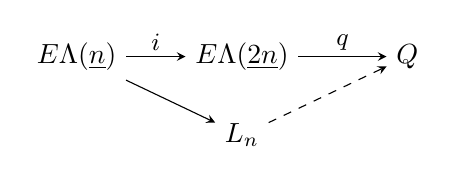
\begin{tikzpicture}[x=7mm,y=5mm]
    \draw[tikzob,mm] %objects
    (0,0) node (0) {\EL(\underline{n})}
    (3,0) node (1) {\EL(\underline{2n})}
    (6,0) node (2) {Q}
    (3,-2) node (d) {L_n};
    \path[tikzar,mm] %arrows
    (0) edge node {i} (1)
    (1) edge node {q} (2)
    (0) edge (d)
    (d) edge[dashed] (2);
%    \draw[tikzob,mm]
%    (0.5,-0.5) node[rotate=270,font=\Large] {\Rightarrow}
%    ++(3mm,0mm) node {v};
  \end{tikzpicture}
  \]
We also have a unique map $\EL(\underline{2n}) \to L_n$ which agrees with the canonical map $\EL(\underline{n}) \to L_n$ on $z_1, \ldots, z_n$ and sends $z_{i+n}$ to the inverse of the image of $z_i$. This gives the diagram below, once again with the dashed arrow induced by the definition of $\delta$ and the universal property.
    \[
  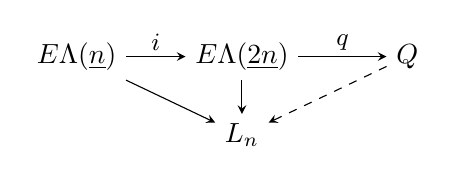
\begin{tikzpicture}[x=7mm,y=5mm]
    \draw[tikzob,mm] %objects
    (0,0) node (0) {\EL(\underline{n})}
    (3,0) node (1) {\EL(\underline{2n})}
    (6,0) node (2) {Q}
    (3,-2) node (d) {L_n};
    \path[tikzar,mm] %arrows
    (0) edge node {i} (1)
    (1) edge node {q} (2)
    (0) edge (d)
    (1) edge (d)
    (2) edge[dashed] (d);
%    \draw[tikzob,mm]
%    (0.5,-0.5) node[rotate=270,font=\Large] {\Rightarrow}
%    ++(3mm,0mm) node {v};
  \end{tikzpicture}
  \]
 The two dashed arrows are then forced to be inverse to each other. 
\end{proof}


\begin{Defi}
We will say that a functor $F: C \to D$ is \emph{surjective}\index{functor!surjective} if the underlying map of graphs is surjective. In particular $F$ must be surjective on objects, but it need not be full.
\end{Defi}

\begin{prop}\label{coeqsurj} Let $\phi, \phi' : X \to Y$ be a pair of $E\Lambda$-algebra maps, and $k: Y \to Z$ their coequalizer in $E\Lambda\mbox{-}\mathrm{Alg}_S$. If the monoid $\mathrm{Ob}(Z)$ is also a group, then the functor $k$ is surjective.
\end{prop}
\begin{proof}
Since the functor $\mathrm{Ob} : E\Lambda\mbox{-}\mathrm{Alg}_S \to \mon$ is a left adjoint, it preserves all colimits so the monoid homomorphism $\mathrm{Ob}(k): \mathrm{Ob}(Y) \to \mathrm{Ob}(Z)$ is the coequalizer of the parallel pair $\mathrm{Ob}(\phi), \mathrm{Ob}(\phi')$ in the category of monoids. Every coequalizer is a regular epimorphism, and in the category of monoids regular epimorphisms coincide with  surjective functions, so $k$ is surjective on objects.


Next, let $f: v \to w$ and $f' : w' \to v'$ be any two morphisms of the category $Y$ for which $k(f)$ and $k(f')$ are composable in $Z$. Since these maps are composable we know that $k(w)$ and $k(w')$ must be the same object of $Z$, and since $\mathrm{Ob}(Z)$ is a group we know this object has an inverse $k(w)^{-1} = k(w')^{-1}$. So by the surjectivity of $k$ we can find another object $y$ of $Y$ for which $k(y) = k(w)^{-1}$. Using this, define the morphism $h: w' \otimes y \otimes v \to v' \otimes y \otimes w$ to be the tensor product $f' \otimes \mathrm{id}_y \otimes f$. Thus
\[ \begin{array}{rll}
		k(h) & = & k(f' \otimes \mathrm{id}_y \otimes f) \\
		& = & k(f') \otimes \mathrm{id}_{k(y)} \otimes k(f) \\
		& = & k(f') \otimes \mathrm{id}_{k(w)^*} \otimes k(f)
		\end{array}
\]
and so by \cref{tenscomp}, this is the composite $k(f') \circ k(f)$. Therefore the set of morphisms of $Z$ which are images of morphisms of $Y$ is closed under composition. 

Now consider $k(Y)$, the subcategory of $Z$ that contains every object $x'$ for which there exists $x$ in $Y$ with $k(x) = x'$, and every morphism $f'$ for which there exists $f$ in $Y$ with $q(f) = f'$. We know that the morphisms of $k(Y)$ are closed under composition, and so this is indeed a well-defined category. It is easy to see that $k(Y)$ is in fact a well-defined sub-$\ML$-monoidal category, and that $k': Y \to k(Y)$ is a surjective strict $\ML$-monoidal functor. This shows that $k'$ coequalizes $\phi, \phi'$, so the inclusion $k(Y) \hookrightarrow Z$ must be an isomorphism and thus $k$ is surjective.
\end{proof}

\begin{rem}\label{alsowithoutgroups}
We note that, since we haven't used any feature of $\ML$ in the above proofs, they all apply equally in the case of no group actions at all, i.e., strict monoidal categories or when $\ML = \mb{T}$ is the terminal action operad consisting only of trivial groups.
\end{rem}



\begin{cor}\label{qsurj} The cokernel map $q: \EL(\underline{2n}) \to L_n$ is surjective.
\end{cor}

\begin{cor}\label{M_coker}
We have an isomorphism of groups as below.
\[ \mathrm{M}(L_n)^{\mathrm{gp},\mathrm{ab}} \quad \cong \quad \bigquotient{\mathrm{M}(\ELnn)^{\mathrm{gp},\mathrm{ab}}}{\mathrm{ker}\big( \, \mathrm{M}(q)^{\mathrm{gp},\mathrm{ab}} \, \big)} \]
\end{cor}


One important consequence of the surjectivity of $q$ is that it will allow us to use some results about the free algebra $\ELnn$ to deduce information about the free invertible algebra $L_n$. In fact, we have done this once already: looking back at \cref{Qobj} with our current knowledge that $Q = L_n$, we can see that it is a direct analogue of \cref{Gnobj}, using the fact that $q$ is surjective on objects. 


QQQ Reference ``Gnmapsaction'' is missing.


In that same vein, one might ask if we can take \cref{Gnmapsaction}, a statement about the morphisms $\ELnn$, and extend it to an analagous result on $L_n$, using surjectivity of $q$ on morphisms instead. That is, since every morphism of $\ELnn$ is an action morphism, and since strict $\ML$-monoidal functors always send action morphisms to action morphisms, we should be able to use $q$ to identify every morphism of $L_n$ as an action morphism. 


QQQ Get some notation for what Ed calls action maps, I don't like all the $\alpha$'s

\begin{nota}\label{newaction}
Let's think about $g^{\otimes}$ for the iso induced by $g$.
\end{nota}

\begin{lem}\label{otimesotimes}
Later I use: $(h \otimes g)^{\otimes} = h^{\otimes} \otimes g^{\otimes}$.
\end{lem}

\begin{lem} \label{allmapsaction} Every morphism in $L_n$ can be expressed as $g^{\otimes}$
for some $g \in \Lambda(m)$ and $x_i \in \{z_1, ..., z_n, z_1^*, ..., z_n^* \}$.
\end{lem}
\begin{proof}
Let $f$ be an arbitrary morphism in $L_n$. By surjectivity of $q$, there must exist at least one morphism $f'$ in $\ELnn$ such that $q(f') = f$, and from \cref{Gnmapsaction} we know that this $f'$ can be expressed uniquely as $g^{\otimes}$ for some $g \in \Lambda(m)$. 
\end{proof}


Note that while this result shows that every morphism of $L_n$ is induced by the action of some $g \in \Lambda(m)$, it does not imply that this $g$ is unique. It will, however, furnish us with all the group actions required to give $L_n$ a $\ML$-monoidal structure once we have given it a mere \emph{monoidal} one using that $q$ is surjective.  QQQ Forward ref to where we accomplish this.

\begin{lem} \label{noscalar} For any element $g \in \Lambda(m), m \in \mathbb{N}$ of an action operad $\ML$, the morphism
\[
g: I^m \to I^m
\]
in $L_n$ is the identity.
Equivalently, for any element $h \in \Lambda(0)$, $h$ induces the identity morphism $I \to I$.
\end{lem}
\begin{proof}
First, let $g \in \Lambda(m)$. Then $g: I^m \to I^m$ is equal to $q(g):q(I^m) \to q(I^m)$ which is equal to $q\delta(g): q\delta(I^m) \to q\delta(I^m)$. Since $q$ is the coequalizer of $\delta$ and the zero map, $q\delta(g) = \id$ for all $g \in \Lambda(m)$. This clearly implies that every $h \in \Lambda(0)$ induces the identity map $I \to I$, but note that the morphism $g:I^m \to I^m$ is also the morphism induced by $\mu(g; e_0, \ldots, e_0) \in \Lambda(0)$, so these two claims are equivalent.
\end{proof}

This is a curious result. The morphisms $I \to I$ in QQQ $n\ML$ vs $\ELn$ QQQ are exactly the elements of the group $\Lambda(0)$, but all of these become the identity in $L_n$. In other words, $L_n$ cannot detect any morphisms in $\Lambda(0)$, an idea we make precise now. 


\begin{prop} \label{G0quot} Let $\Lambda$ be a crossed action operad. Then there exists another crossed action operad $\Lambda'$ given by $\Lambda'(m) = \Lambda(m)/\Lambda(0)$ for all $m \in \mathrm{N}$.
\end{prop}
\begin{proof}
For any elements $g \in \Lambda(m)$ and $h \in \Lambda(0)$, their tensor product $h \otimes g := \mu(e_2; h, g)$ is also an element of $\Lambda(m)$. This defines a map $\Lambda(0) \times \Lambda(m) \to \Lambda(m)$, which is both a group homomorphism and a group action by \cref{G0abel}. This produces a homomorphism $\Lambda(0) \to \Lambda(m)$ for all $m$ which lies in the center of $\Lambda(m)$ by QQQ \cref{spacial}, hence is normal for all $m$. Furthermore, the induced map $\Lambda(0) \to \Lambda(m) \to \Sigma_m$ is the zero map, so we have an induced homomorphism $\Lambda(m)/\Lambda(0) \to \Sigma_m$. All that remains to be shown is that we the operadic multiplication for $\Lambda$ induces one for the groups $\Lambda(n)/\Lambda(0)$, and that this multiplication satisfies the axioms for an action operad.

Let $h, h_1, ..., h_m \in \Lambda(0)$ and $k_1, ..., k_m \in \mathbb{N}$. We have the following calculation using the action operad axioms for $\Lambda$ and the fact that $\EL(\underline{1})$ is spacial (see \cref{spacial}) so the $e_k$ commute with all elements of $\Lambda(0)$.
\[ \begin{array}{rll}
		\mu^{\Lambda}( \, h \otimes e_m \, ; \, h_1 \otimes e_{k_1}, ..., h_m \otimes e_{k_m} \, ) & = & \mu^{\Lambda}\big( \, \mu^{\Lambda}(e_2; h, e_m) \, ; \, h_1 \otimes e_{k_1}, ..., h_m \otimes e_{k_m} \, \big) \\
		& = & \mu^{\Lambda}\big( \, e_2 \, ; \, \mu^{\Lambda}(h;-), \mu^{\Lambda}(e_m; h_1 \otimes e_{k_1}, ..., h_m \otimes e_{k_m}) \, \big) \\
		& = & \mu^{\Lambda}(h;-) \otimes \mu^{\Lambda}(e_m; h_1 \otimes e_{k_1}, ..., h_m \otimes e_{k_m})  \\
		& = & h \otimes h_1 \otimes e_{k_1} \otimes ... \otimes h_m \otimes e_{k_m} \\
		& = & e_{k_1} \otimes ... \otimes e_{k_m} \otimes h \otimes h_1 ... \otimes h_m \\
		& = & e_{k_1+...+k_m} \otimes h \otimes h_1 ... \otimes h_m
		\end{array}
\]
This shows that the square below commutes.
\begin{center}
    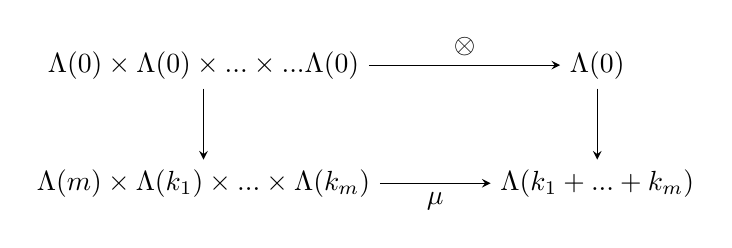
\begin{tikzpicture}[x=50mm,y=15mm]
		\node (a) at (0,0) {$ \Lambda(0) \times  \Lambda(0) \times ... \times ...  \Lambda(0)$};
		\node (b) at (1,0) {$\Lambda(0)$};
		\node (c) at (0,-1) {$ \Lambda(m) \times  \Lambda(k_1) \times ... \times  \Lambda(k_m) $};
		\node (d) at (1,-1) {$\Lambda(k_1 + ... + k_m)$};
			\draw [->] (a) to node [above] {$\otimes$} (b);
			\draw [->] (b) to node [right] {$$} (d);
			\draw [->] (a) to node [left] {$$} (c);
			\draw [->] (c) to node [below] {$\mu$} (d);
    \end{tikzpicture}
\end{center}	

We write the image of $g \in \Lambda(m)$ under the quotient $\Lambda(m) \to \Lambda'(m)$ as $[g]$. We will show that the multiplication
\[
\mu^{\Lambda'}:\Lambda'(m) \times \Lambda'(k_1) \times \cdots \times \Lambda'(k_m) \to \Lambda'(k_1 + \cdots + k_m)
\]
given by 
\[
\mu^{\Lambda'}\Big( [g]; [g_1], \ldots , [g_m] \Big) = [\mu^{\Lambda}\Big(g; g_1, \ldots, g_m \Big)]
\]
is well-defined. With $h, h_1, ..., h_m \in \Lambda(0)$ as above, we have
\[
\mu^{\Lambda}\Big(g \cdot h \otimes e_m; g_1\cdot h_1 \otimes e_{k_1}, \ldots, g_m\cdot h_m \otimes e_{k_m} \Big) \mu^{\Lambda}(g; g_1, \ldots, g_m) \cdot \mu^{\Lambda}(h \otimes e_m; \cdot h_1 \otimes e_{k_1}, \ldots, \cdot h_m \otimes e_{k_m})
\]
using the fact that $\pi(h \otimes e_m)$ is the identity permutation. By the commutative square above, $\mu^{\Lambda}(h \otimes e_m; \cdot h_1 \otimes e_{k_1}, \ldots, \cdot h_m \otimes e_{k_m})$ is in the image of $\Lambda(0) \to \Lambda(k_1 + \cdots + k_m)$, so $\mu^{\Lambda'}$ is well-defined. It is now straightforward to check the rest of the action operad axioms for $\Lambda'$ using those of $\Lambda$.
\end{proof}

For crossed $\Lambda$, this notion of quotient by $\Lambda(0)$ does exactly what we wanted it to do --- remove certain information which is unnecessary for forming the algebra $L_n$. We will use this later in QQQ for something.

\begin{prop} \label{noscalarcross} Let $\Lambda$ be a crossed action operad, and let $\Lambda'$ be the action operad with $\Lambda'(m) = \Lambda(m)/\Lambda(0)$ constructed in \cref{G0quot}. Then for any $n \in \mathrm{N}$,
\[ L\ML'_n \quad \cong \quad L\ML_n \]
both as $E\Lambda$-algebras and as $E\Lambda'$-algebras.  
\end{prop}
\begin{proof}

The quotient map $[-]:\ML \to \ML'$ induces a $\ML$-algebra structure on $L\ML'_n$, and hence produces a unique strict $\ML$-monoidal functor $L\ML_n \to L\ML'_n$ by the universal property of $L\ML_n$. $L\ML_n$ is also a $\ML'$-monoidal category by defining $[g]^{\otimes} : x_1 \otimes \cdots \otimes x_n \to x_{[g]^{-1}1} \otimes \cdots \otimes x_{[g]^{-1}n}$ to be $g^{\otimes}$. This is well-defined, as whenever we have $[g] = [h]$ it is because there is some $x \in \ML(0)$ for which $h = x \otimes g = \mu_2(e_2; x, g)$. Then
\[
h^{\otimes} = (x \otimes g)^{\otimes} = x^{\otimes} \otimes g^{\otimes} = \id_I \otimes g^{\otimes} = g^{\otimes}
\]
using \cref{otimesotimes}. Thus we also have an induced map $L\ML'_n \to L\ML_n$ using the universal property of $L\ML'_n$. By inspection, both of these functors preserve the $\ML$- and $\ML'$-actions, hence must be inverse to each other.
\end{proof}

I am taking out the $G(1)$-generated stuff for now.


Just note everything is true for monoidal categories, \cref{alsowithoutgroups}.

\begin{nota}\label{plus_notation}
Let $f: A \to C, g: B \to C$ be maps in a category with coproducts. We will write $f;g: A \coprod B \to C$ for the unique map induced by the universal property of the coproduct.
\end{nota}

\begin{lem}\label{sum_coeq}
Let $f, g: A \to B$ be maps in a cocomplete category with coequalizer $c: B \to C$. Then $c$ is also the coequalizer of $f;\id_B$ and $g; \id_B$.
\end{lem}
\begin{proof}
A map $h: B \to X$ coequalizes $f;\id_B$ and $g; \id_B$ if and only if $hf = hg$ and $h \id_B = h \id_B$ by the universal property of the coproduct, so $c$ is still the universal map which coequalizes.

\end{proof}

\begin{Defi} \label{coprodmapdef} Let $\tilde{\delta} = \mathrm{id}_{\ELnn};\delta$.
Explicitly, $\tilde{\delta}$ is the map of $E\Lambda$-algebras which acts on generators by
\[ \begin{array}{rlrlll}
			\tilde{\delta} & : & \ELnnnn & \to & \ELnn \\
			&  & z_i & \mapsto & z_i  \\
			&  & z_{n+i} & \mapsto & z_{n+i} \\
			&  & z_{2n+i} & \mapsto & z_i \otimes z_{n+i} \\
			&  & z_{3n+i} & \mapsto & z_{n+i} \otimes z_i			
		\end{array}
\]
for $1 \le i \le n$. Similarly, let $\tilde{I} = \mathrm{id}_{\ELnn};I$.
Explicitly, $\tilde{I}$ is the map of $E\Lambda$-algebras which acts on generators by
\[ \begin{array}{rlrlll}
			\tilde{I} & : & \ELnnnn & \to & \ELnn \\
			&  & z_i & \mapsto & z_i  \\
			& & z_{n+i} & \mapsto & z_{n+i} \\
			& & z_{2n+i} & \mapsto & I \\
			&  & z_{3n+i} & \mapsto & I
		\end{array} 
\]
for $1 \le i \le n$. 
\end{Defi}



\begin{cor}\label{q_other_coeq} The functor $q$ (\cref{qdef}) is the coequalizer of $\tilde{\delta}$ and $\tilde{I}$ in $E\Lambda\mbox{-}\mb{Alg}_S$.
\end{cor}

By construction, $\tilde{\delta}$ and $\tilde{I}$ form a reflexive pair in $E\Lambda\mbox{-}\mb{Alg}_S$, so by \cref{refcoeq_calcs} we have the further corollary below.

\begin{cor}\label{q_other_coeq2} The functor $q$  is the coequalizer of $\tilde{\delta}$ and $\tilde{I}$ in $\moncat$ or in $\cat$.
\end{cor}

Now that we can  express the map $q: \ELnn \to L_n$ as a colimit of mere monoidal categories, we can use the adjunction from \cref{Moradj} to calculate $\mathrm{M}(L_n)^{\mathrm{gp},\mathrm{ab}}$. 

QQQ Need to think about the $f^*$ below

\begin{prop}\label{Zmor2} Let $\Delta$ be the subgroup of $\mathrm{M}(\ELnn)^{\mathrm{gp, ab}}$ generated by elements of the form
\[ \mathrm{M}(\tilde{\delta})^{\mathrm{gp, ab}}(f) \, \otimes \, \mathrm{M}(\tilde{I})^{\mathrm{gp, ab}}(f)^*, \quad \quad \quad f \in \mathrm{M}(\ELnnnn)^{\mathrm{gp, ab}} \]
Then the abelianization of the group completion of the collapsed morphisms of $L_n$ is 
\[ \mathrm{M}(L_n)^{\mathrm{gp, ab}} \quad = \quad \bigquotient{{\mathrm{M}(\ELnn)}^{\mathrm{gp, ab}}}{\Delta} \]
with $\mathrm{M}(q)^{\mathrm{gp, ab}}$ acting as the appropriate quotient map. 
\end{prop}
\begin{proof}
From \cref{Moradj}, we know that $\mathrm{M}(\, \_ \,)^{\mathrm{gp, ab}}: \moncat \to \mathrm{Ab}$ is a left adjoint functor. This means that it preserves all colimits in $\moncat$, so
\[ \mathrm{coeq}\big( \, \mathrm{M}(\tilde{\delta})^{\mathrm{gp, ab}}, \, \mathrm{M}(\tilde{I})^{\mathrm{gp, ab}} \, \big) \quad \cong \quad \mathrm{M}\big( \, \mathrm{coeq}(\tilde{\delta}, \tilde{I}) \, \big)^{\mathrm{gp, ab}} \quad \cong \quad \mathrm{M}(q)^{\mathrm{gp, ab}}. \]

The coequalizer of two abelian group homomorphisms is just the quotient of their common target by the image of their difference. Hence in this case we have
\[ 
\begin{array}{rcl}
\mathrm{M}(L\mathbb{G}_{n})^{\mathrm{gp, ab}}  & \cong &  \bigquotient{{\mathrm{M}(\ELnn)}^{\mathrm{gp, ab}}}{\mathrm{im}\big( \, {\mathrm{M}(\tilde{\delta})}^{\mathrm{gp, ab}} - {\mathrm{M}(\tilde{I})}^{\mathrm{gp, ab}} \, \big)} \\
& \cong & \quad \bigquotient{{\mathrm{M}(\ELnn)}^{\mathrm{gp, ab}}}{\Delta}.
\end{array}
\]
\end{proof} 

\begin{rem}\label{delta_neq_image}
Note that $\mathrm{im}(\mathrm{M}(\delta)^{\mathrm{gp, ab}})$ is a subgroup of $\Delta$ because $\delta$ factors through $\tilde{\delta}$.
\end{rem}



QQQ I actually don't know the purpose of this lemma yet.

Our goal is to explicitly compute the group acting on a set of $n$ invertible objects in a $\ML$-monoidal category, so we will need an explicit description of the elements of the subgroup $\Delta$.

\begin{lem} $\Delta$ is the subgroup of $\mathrm{M}(\ELnn)^{\mathrm{gp, ab}}$ whose elements are tensor products of equivalence classes
\[ \begin{array}{c}
			\big[ \, \alpha^{\ELnn}\big( \, \mu( \, g \, ; \, e_{|\tilde{\delta}(x_1)|}, ..., e_{|\tilde{\delta}(x_m)|} \, ) \, ; \, \mathrm{id}_{x'_1}, ...,  \mathrm{id}_{x'_{m'}} \, \big) \, \big] \\
			\, \otimes \, \\
			\big[ \, \alpha^{\ELnn}\big( \, \mu( \, g \, ; \, e_{|\tilde{I}(x_1)|}, ..., e_{|\tilde{I}(x_m)|} \, ) \, ; \, \mathrm{id}_{x''_1}, ...,  \mathrm{id}_{x''_{m''}} \, \big) \, \big]^*
		\end{array}
\] 
where $g \in G(m)$, the $x_i$ are generators of $\mathbb{N}^{\ast 4n}$, the $x'_i, x''_i$ are generators of $\mathbb{N}^{\ast 2n}$, and
\[ \begin{array}{rll}
			\tilde{\delta}( x_1 \otimes ... \otimes x_m) & = & x'_1 \otimes ... \otimes x'_{m'} \\
			\tilde{I}( x_1 \otimes ... \otimes x_m) & = & x''_1 \otimes ... \otimes x''_{m''}
		\end{array}
\]
\end{lem}
\begin{proof}  
Let $f$ be an element of $\mathrm{M}(\mathbb{G}_{4n})^{\mathrm{gp, ab}}$. By definition this means that $f$ is an equivalence class of morphisms from $\mathbb{G}_{4n}$, and so by \cref{Gnmapsaction} there must exist $g \in G(m)$ and $x_1, ..., x_m \in \{ z_1, ..., z_{4n} \}$ for which
\[ f \quad = \quad [ \, \alpha^{\mathbb{G}_{4n}}(g; \mathrm{id}_{x_1}, ..., \mathrm{id}_{x_m}) \, ] \]
Thus
\[ \begin{array}{rll}
			\mathrm{M}(\tilde{\delta})^{\mathrm{gp, ab}}(f) & = & \mathrm{M}(\tilde{\delta})^{\mathrm{gp, ab}} \big( \, [ \, \alpha^{\mathbb{G}_{4n}}(g; \mathrm{id}_{x_1}, ..., \mathrm{id}_{x_m}) \, ] \, \big) \\
			& = & \big[ \, \tilde{\delta}\big( \, \alpha^{\mathbb{G}_{4n}}(g; \mathrm{id}_{x_1}, ..., \mathrm{id}_{x_m}) \, \big) \, \big]  \\
			& = & [ \, \alpha^{\ELnn}(g; \mathrm{id}_{\tilde{\delta}(x_1)}, ..., \mathrm{id}_{\tilde{\delta}(x_m)}) \, ]
		\end{array}
\]
But again using \cref{Gnmapsaction}, we know it must be possible to express the action morphism $\alpha^{\ELnn}(g; \mathrm{id}_{\tilde{\delta}(x_1)}, ..., \mathrm{id}_{\tilde{\delta}(x_m)})$ as an action morphism on the identities of generators. Since the source of this map is
\[ \tilde{\delta}(x_1) \otimes ... \otimes \tilde{\delta}(x_m) \quad = \quad \tilde{\delta}(x_1 \otimes ... \otimes x_m) \quad =: \quad x'_1 \otimes ... \otimes x'_{m'}  \]
clearly the $x'_i$ are the generators we want, and so by expanding the $\tilde{\delta}(x_i)$ as tensor products of these we find that
\[ [ \, \alpha^{\ELnn}(g; \mathrm{id}_{\tilde{\delta}(x_1)}, ..., \mathrm{id}_{\tilde{\delta}(x_m)})  \, ] \quad = \quad \big[ \, \alpha^{\ELnn}\big( \, \mu( \, g \, ; \, e_{|\tilde{\delta}(x_1)|}, ..., e_{|\tilde{\delta}(x_m)|} \, ) \, ; \, \mathrm{id}_{x'_1}, ..., \mathrm{id}_{x'_{m'}} \, \big) \, \big] \]
For analogous reasons we also get
\[ \begin{array}{rll}
			\mathrm{M}(\tilde{I})^{\mathrm{gp, ab}}(f) & = & [ \, \alpha^{\ELnn}(g; \mathrm{id}_{\tilde{I}(x_1)}, ..., \mathrm{id}_{\tilde{I}(x_m)}) \, ]  \\
			& = &  \big[ \, \alpha^{\ELnn}\big( \, \mu( \, g \, ; \, e_{|\tilde{I}(x_1)|}, ..., e_{|\tilde{I}(x_m)|} \, ) \, ; \, \mathrm{id}_{x''_1}, ...,  \mathrm{id}_{x''_{m''}} \, \big) \, \big]
		\end{array}
\]
and using these equations the lemma follows immediately from the definition of $\Delta$.
\end{proof}



\section{Sources and targets in \texorpdfstring{$L_n$}{L_n}}   

\begin{Defi}\label{st} For any $E\Lambda$-algebra $X$, denote by $s: \mathrm{Mor}(X) \to \mathrm{Ob}(X)$ and $t: \mathrm{Mor}(X) \to \mathrm{Ob}(X)$ the monoid homomorphisms which send each morphism of $X$ to its source and target, respectively. That is,
\[ s( \, f: x \to y) \, = \, x, \quad \quad t( \, f: x \to y) \, = \, y. \]
\end{Defi}


\begin{lem}\label{stmon} Let $X$ be an $E\Lambda$-algebra whose underlying category is a groupoid, and $s \times t: \mathrm{Mor}(X) \to \mathrm{Ob}(X)^2$ the map induced from $s$ and $t$ using the universal property of products. Then the image of this map is
\[ (s \times t)(X) \, = \, \mathrm{Ob}(X) \times_{\pi_0(X)} \mathrm{Ob}(X) \]
where this pullback is taken over the canonical maps sending objects of $X$ to their connected components:
\[ \begin{tikzcd}
\mathrm{Ob}(X) \times_{\pi_0(X)} \mathrm{Ob}(X) \ar[dd, shift left=12] \ar[rr] \ar[ddrr, phantom, "\lrcorner", near start, shift left=4] & & \mathrm{Ob}(X) \ar[dd, "\lbrack \, \_ \, \rbrack"] & \\ 
& & & \\
\quad \quad \quad \quad \quad \quad \mathrm{Ob}(X) \ar[rr, "\lbrack \, \_ \, \rbrack"] & & \pi_0(X)
\end{tikzcd} \]
\end{lem} 


Recalling \cref{Gnobj,Gnconcomp,Zobj,crossconcomp}, we can immediately conclude the following.

\begin{cor} \label{stpullback}
\[\begin{array}{rll} 
		(s \times t)(\ELn) & \cong & \begin{cases}
								\quad \mathbb{N}^{\ast n} \times_{\mathbb{N}^n} \mathbb{N}^{\ast n} & \text{if $G$ is crossed}\\
								\quad \mathbb{N}^{\ast n} & \text{otherwise}
							\end{cases} \\
		& & \\
		(s \times t)(L_n) & \cong & \begin{cases}
								\quad \mathbb{Z}^{\ast n} \times_{\mathbb{Z}^n} \mathbb{Z}^{\ast n}  & \text{if $G$ is crossed}\\
								\quad \mathbb{Z}^{\ast n} & \text{otherwise}
							\end{cases} \\
		\end{array}
\]
where the pullbacks are taken over the quotients of abelianization for $(\mathbb{N}^{\ast n})^{\mathrm{ab}} = \mathbb{N}^n$ and $(\mathbb{Z}^{\ast n})^{\mathrm{ab}} = \mathbb{Z}^n$ respectively.
\end{cor}

Next, we want to show that this $(s \times t)(L_n)$ we have described is in fact a submonoid of $\mathrm{Mor}(L_n)$.  We will accomplish this  by first proving the analogous statement for all $\ELn$, and then recovering the $L_n$ version from it later.  For any pair $(w, w') \in \mathbb{N}^{\ast n} \times_{\mathbb{N}^n} \mathbb{N}^{\ast n}$ such that the images of $w$ and $w'$ in the commutative monoid $\mathbb{N}^n$ are the same, there are generators $x_1, ..., x_m$ for which 
\[ w \quad = \quad x_1 \otimes ... \otimes x_m \]
and there exists at least one permutation $\sigma \in S_m$ such that
\[ w' \quad = \quad x_{\sigma(1)} \otimes ... \otimes x_{\sigma(m)}. \]
Since the underlying permutation maps $\pi : G(m) \to \mathrm{S}_m$ of a crossed action operad $G$ are all surjective, we can always find an element of $g \in G(m)$ for which $\pi(g) = \sigma$. 

\begin{nota}\label{rho_ww'}
Let $\rho:\mathbb{N}^{\ast n} \times_{\mathbb{N}^n} \mathbb{N}^{\ast n} \to \bigcup \EL(m)$ be an arbitrary, but fixed, function such that $\rho(w,w')$ satisfies $\pi(\rho(w,w')) = \sigma$ as defined above.
\end{nota}



\begin{lem}\label{freemon} $\mathbb{N}^{\ast n} \times_{\mathbb{N}^n} \mathbb{N}^{\ast n}$ is a free monoid.
\end{lem}
\begin{proof}
Write the generators for the first copy of $\mathbb{N}^{\ast n}$ in $\mathbb{N}^{\ast n} \times_{\mathbb{N}^n} \mathbb{N}^{\ast n}$ as $a_1, \ldots, a_n$, and the generators for the second copy of $\mathbb{N}^{\ast n}$ as $x_1, \ldots, x_n$. An element $(w,w') \in \mathbb{N}^{\ast n} \times_{\mathbb{N}^n} \mathbb{N}^{\ast n}$ can therefore be written uniquely as
\[
(w,w') = (a_{i_1} a_{i_2} \cdots a_{i_k}, x_{i_1} x_{i_2} \cdots x_{i_j})
\]
and being an element of the pullback immediately implies $k=j$. We then define an element $ (a_{i_1} a_{i_2} \cdots a_{i_k}, x_{i_1} x_{i_2} \cdots x_{i_k})$ of $\mathbb{N}^{\ast n} \times_{\mathbb{N}^n} \mathbb{N}^{\ast n}$ to be indecomposable if there does not exist an $h < k$ such that $ (a_{i_1} a_{i_2} \cdots a_{i_h}, x_{i_1} x_{i_2} \cdots x_{i_h})$ is also an element of $\mathbb{N}^{\ast n} \times_{\mathbb{N}^n} \mathbb{N}^{\ast n}$. It is clear that every element can be written as a product of indecomposables. If $(w,w')$ can be written as a product of indecomposables in two ways, say 
\[
(w,w') = c_1 \cdots c_s = d_1 \cdots d_t,
\]
then the length (QQQ we defined this kind of thing somewhere) of $c_1$ must be either strictly less than or strictly greater than the length of $d_1$; if they had equal length, then they would be equal. Without loss of generality assume $c_1$ has length $l_c$ which is strictly less than the length $l_d$ of $d_1$. But then the first $l_c$ terms appearing in $d_1$ would agree with $c_1$, proving that $d_1$ is not indecomposable. Straightforward induction then finishes the proof that every element of $\mathbb{N}^{\ast n} \times_{\mathbb{N}^n} \mathbb{N}^{\ast n}$ can be written as a product of indecomposables in a unique way, making $\mathbb{N}^{\ast n} \times_{\mathbb{N}^n} \mathbb{N}^{\ast n}$ free on the set of indecomposables.
\end{proof}

We can now construct the desired injection using the function $\rho$ from \cref{rho_ww'}.
\begin{prop} \label{stGnsub} $\mathrm{Mor}(\ELn) \to (s \times t)(\ELn)$ is a split epi of monoids, so $(s \times t)(\ELn)$ is (isomorphic to) a submonoid of $\mathrm{Mor}(\ELn)$. Furthermore, we can choose the injection $i:(s \times t)(\ELn) \to \mathrm{Mor}(\ELn)$ such that the following diagram commutes.
\begin{center}
    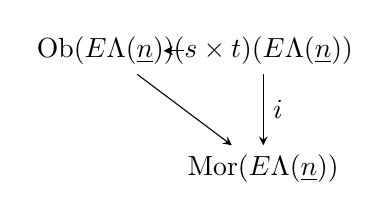
\begin{tikzpicture}[x=20mm,y=15mm]
		\node (a) at (0,0) {$\mathrm{Ob}(\ELn)$};
		\node (b) at (1,0) {$(s \times t)(\ELn)$};
		\node (d) at (1,-1) {$\mathrm{Mor}(\ELn)$};
      \draw [->] (a) to (b);
			\draw [->] (a) to node [above] {$$} (b);
			\draw [->] (b) to node [right] {$i$} (d);
			\draw [->] (a) to node [below,left] {$$} (d);
    \end{tikzpicture}
\end{center}		
\end{prop}
\begin{proof}
First, assume that the action operad $G$ is non-crossed. Then there exists an obvious injective monoid homomorphism
\[ \begin{array}{rlrll}
			i & : & (s \times t)(\ELn) & \to & \mathrm{Mor}(\ELn) \\
			& : & \mathbb{N}^{\ast n} & \to & G \times_{\mathbb{N}} \mathbb{N}^{\ast n} \\
			& : & w & \mapsto & ( \, e_{|w|}, w \, )
		\end{array}
\]
The homomorphism property follows from the fact that the length $|w|$ defined in \cref{lengthdef} is itself a homomorphism, so $|w \otimes w'| = |w|+|w'|$. Thus $(s \times t)(\ELn) \subseteq \mathrm{Mor}(\ELn)$ for non-crossed $G$.

Now assume that $G$ is crossed. Fix a function $\rho$ as in \cref{rho_ww'}. Because $\mathbb{N}^{\ast n} \times_{\mathbb{N}^n} \mathbb{N}^{\ast n}$ is a free monoid  by \cref{freemon}, there is a unique monoid homomorphism
\[ \rho \, : \, \mathbb{N}^{\ast n} \times_{\mathbb{N}^n} \mathbb{N}^{\ast n} \longrightarrow G \]
which agrees with the original function $\rho$ on the generators in the source. By construction, we have
\[ \pi(\rho(w, w'))(w) \quad = \quad w' \]
for any $(w, w') \in\mathbb{N}^{\ast n} \times_{\mathbb{N}^n} \mathbb{N}^{\ast n}$, not just the generators. Using $\rho$ we define the homomorphism $i$ to be
\[ \begin{array}{rlrll}
			i & : & (s \times t)(\ELn) & \to & \mathrm{Mor}(\ELn) \\
			&  & \mathbb{N}^{\ast n} \times_{\mathbb{N}^n} \mathbb{N}^{\ast n} & \to & G \times_{\mathbb{N}} \mathbb{N}^{\ast n} \\
			&  & (w, w') & \mapsto & ( \, \rho(w, w'), w \, ).
		\end{array}
\]
Moreover, for any two elements $(v, v')$, $(w, w')$ of $\mathbb{N}^{\ast n} \times_{\mathbb{N}^n} \mathbb{N}^{\ast n}$ we have
\[ \begin{array}{lcl}
		( \, \rho(v, v'), v \, )  =  ( \, \rho(w, w'), w \, ) & \implies & \rho(v, v') \, = \, \rho(w, w'), \quad \quad v \, = \, w \\
		 & \implies & v' \, = \, \pi(\rho(v, v'))(v) \, = \, \pi(\rho(w, w'))(w) \, = \, w'
		\end{array}
\]
and thus $i$ is injective. This injection splits $\mathrm{Mor}(\ELn) \to (s \times t)(\ELn)$ by construction.

For the final statement, note that the inclusion of $\mathrm{Ob}(\ELn)$ into $(s \times t)(\ELn)$ sends an object $w$ to the pair $(w,w)$. The only indecomposable such are $(x_i, x_i)$ if we write the generating objects of $\ELn$ as $x_1, x_2, \ldots, x_n$. Using the construction above, we can always choose $\rho(x_i, x_i) = e_1$.
\end{proof}


For the proof of \cref{stGnsub}, $\rho$ can be any function satisfying the criteria in \cref{rho_ww'}, with the caveat that commuting with the inclusion of objects requires $\rho(x_i, x_i) = e_1$. The analogous proof for $L_n$, though, requires more properties of $\rho$ which we establish now. Recall the functor $\delta$ from \cref{qdef}.

\begin{lem}\label{rho_lemmas}
If $(w,w') \in \mathbb{N}^{\ast n} \times_{\mathbb{N}^n} \mathbb{N}^{\ast n}$ is indecomposable, then so is $\delta(w,w')$. For any indecomposable $(w,w')$, there exists a unique natural number $k$ and indecomposable $(v,v')$ such that
\[
(w,w') = \delta^k(v,v')
\]
but $(v,v')$ is not $\delta(u,u')$ for any indecomposable $(u,u')$.
\end{lem}
\begin{proof}
The first statement follows immediately from the injectivity of $\delta$ on objects, and the second from the fact that $\delta$ doubles the length of any element.
\end{proof}


\begin{prop} \label{stZsub} $\mathrm{Mor}(L_n) \to (s \times t)(L_n)$ is a split epi of monoids, so $(s \times t)(L_n)$ is (isomorphic to) a submonoid of $\mathrm{Mor}(L_n)$. Furthermore, we can choose the injection $i:(s \times t)(L_n) \to \mathrm{Mor}(L_n)$ such that the following diagram commutes.
\begin{center}
    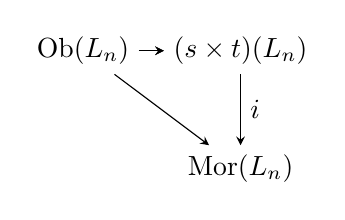
\begin{tikzpicture}[x=20mm,y=15mm]
		\node (a) at (0,0) {$\mathrm{Ob}(L_n)$};
		\node (b) at (1,0) {$(s \times t)(L_n)$};
		\node (d) at (1,-1) {$\mathrm{Mor}(L_n)$};
      \draw [->] (a) to (b);
			\draw [->] (a) to node [above] {$$} (b);
			\draw [->] (b) to node [right] {$i$} (d);
			\draw [->] (a) to node [below,left] {$$} (d);
    \end{tikzpicture}
\end{center}		
\end{prop}
\begin{proof}
Let $i:(s \times t)(\ELnn) \to \mathrm{Mor}(\ELnn)$ be a splitting as in \cref{stGnsub}. We will first show that the function $\rho$ can be chosen to make the square
\begin{center}
    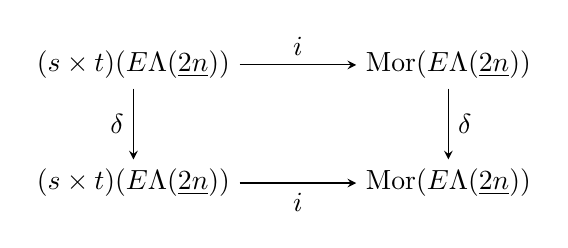
\begin{tikzpicture}[x=20mm,y=15mm]
		\node (a) at (0,0) {$(s \times t)(\ELnn)$};
		\node (b) at (2,0) {$\mathrm{Mor}(\ELnn)$};
		\node (c) at (0,-1) {$(s \times t)(\ELnn) $};
		\node (d) at (2,-1) {$\mathrm{Mor}(\ELnn)$};
			\draw [->] (a) to node [above] {$i$} (b);
			\draw [->] (b) to node [right] {$\delta$} (d);
			\draw [->] (a) to node [left] {$\delta$} (c);
			\draw [->] (c) to node [below] {$i$} (d);
    \end{tikzpicture}
\end{center}
commute. Recall that $i$ is defined by first factoring an element into decomposables, and then applying $\rho$ to each of those. Thus on an indecomposable $(w,w')$, the commutativity of this square is the claim that $\delta(\rho(w,w')) = \rho(\delta w, \delta w')$ using that $\delta(w,w') = (\delta w, \delta w')$ is also indecomposable by the first part of \cref{rho_lemmas}. By the second part of \cref{rho_lemmas}, write $(w,w') = \delta^k(v,v')$, so we need
\[
\delta(\rho(\delta^k(v,v'))) = \delta^{k+1}\rho(v,v').
\]
Furthermore, $(v,v')$ cannot be written as $\delta(u,u')$ for any indecomposable $(u,u')$, so we may choose $\rho(v,v')$ arbitrarily and this will uniquely determine $i$ in such a way that the square commutes. 

The functor $q:\ELnn \to L_n$ is the cokernel of $\delta$, so the composite
\[
\mathrm{Mor}(\ELnn) \stackrel{\mathrm{Mor}\delta}{\longrightarrow} \mathrm{Mor}(\ELnn) \stackrel{\mathrm{Mor}q}{\longrightarrow} \mathrm{Mor}(L_n)
\]
is the zero map. From the definition of $\delta$ in \cref{qdef} and the description of the monoids $(s \times t)(\ELn), (s \times t)(L_n)$ in \cref{stpullback}, the composite
\[
(s \times t)(\ELnn) \stackrel{(s \times t)(\delta)}{\longrightarrow}  (s \times t)(\ELnn) \stackrel{(s \times t)(q)}{\longrightarrow} (s \times t)(L_n)
\]
exhibits $(s \times t)(L_n)$ as the cokernel of $(s \times t)(\delta)$ which induces a unique monoid homomorphism $i: (s \times t)(L_n) \to \mathrm{Mor}(L_n)$ making the square below commute.
\begin{center}
    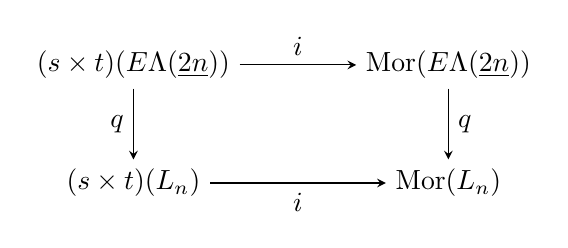
\begin{tikzpicture}[x=20mm,y=15mm]
		\node (a) at (0,0) {$(s \times t)(\ELnn)$};
		\node (b) at (2,0) {$\mathrm{Mor}(\ELnn)$};
		\node (c) at (0,-1) {$(s \times t)(L_n) $};
		\node (d) at (2,-1) {$\mathrm{Mor}(L_n)$};
			\draw [->] (a) to node [above] {$i$} (b);
			\draw [->] (b) to node [right] {$q$} (d);
			\draw [->] (a) to node [left] {$q$} (c);
			\draw [->] (c) to node [below] {$i$} (d);
    \end{tikzpicture}
\end{center}
This homomorphism $i$ splits $\mathrm{Mor}(L_n) \to (s \times t)(L_n)$ as desired.

The final claim about commuting with the inclusion of objects follows using the same argument as in  \cref{stGnsub}, so we must also require $\rho(x_i, x_i) = e_1$.

\end{proof} 

\section{Unit endomorphisms of \texorpdfstring{$L_n$}{L_n}}

We now consider the monoid of unit endomorphisms, $L_n(I,I)$. This is a particularly important submonoid of the morphisms $\mathrm{Mor}(L_n)$, since it is the only submonoid which is also a homset of the category $L_n$. Moreover, because the maps in $L_n(I,I)$ all share the same source and target, what we have is not just a monoid under tensor product but also under composition as well. This fact leads to a series of special properties for $L_n(I,I)$, the first of which is just another instance of the classic Eckmann-Hilton argument. QQQ Reference here?

\begin{prop} \label{endcom} $L_n(I,I)$ is a commutative monoid under both tensor product and composition, with $f \otimes f' = f \circ f'$. Since $L_n$ is a groupoid, this commutative monoid is actually an abelian group.
\end{prop}

Indeed, by using a slightly broader argument we can extend this result to every morphism of $L_n$.

\begin{prop} \label{tensinv} Every morphism $f: w \to v$ in $L_n$ has an inverse under tensor product, $f^*: w^* \to v^*$. That is, the monoid $\mathrm{Mor}(L_n)$ is actually a group.
\end{prop}
\begin{proof}
For any $f: w \to v$ in $L_n$, consider the map $\mathrm{id}_{w^*} \otimes f^{-1} \otimes \mathrm{id}_{v^*}$, where $f^{-1}$ is the compositional inverse of $f$, as in the proof of \cref{endab}. This morphism has source $w^* \otimes v \otimes v^* = w^*$ and target $w^* \otimes w \otimes v^* = v^*$, which allows us to apply the law of interchange to get
\begin{longtable}{RLL}
			f \otimes (\mathrm{id}_{w^*} \otimes f^{-1} \otimes \mathrm{id}_{v^*}) & = & \big( \, f \circ \mathrm{id}_w \, \big) \otimes \big( \, \mathrm{id}_{v^*} \circ  (\mathrm{id}_{w^*} \otimes f^{-1} \otimes \mathrm{id}_{v^*}) \, \big) \\
			& = & \big( \, f \otimes \mathrm{id}_{v^*} \, \big) \circ \big( \, \mathrm{id}_w \otimes (\mathrm{id}_{w^*} \otimes f^{-1} \otimes \mathrm{id}_{v^*}) \, \big) \\
			& = & ( f \otimes \mathrm{id}_{v^*} ) \circ ( f^{-1} \otimes \mathrm{id}_{v^*}) \\
			& = & \mathrm{id}_I
\end{longtable}
and 
\begin{longtable}{RLL}
			(\mathrm{id}_{w^*} \otimes f^{-1} \otimes \mathrm{id}_{v^*}) \otimes f & = & \big( \, (\mathrm{id}_{w^*} \otimes f^{-1} \otimes \mathrm{id}_{v^*}) \circ \mathrm{id}_{w^*} \, \big) \otimes \big( \, \mathrm{id}_v \circ f \, \big) \\
			& = & \big( \, (\mathrm{id}_{w^*} \otimes f^{-1} \otimes \mathrm{id}_{v^*}) \otimes \mathrm{id}_v \, \big) \circ \big( \, \mathrm{id}_{w^*} \otimes f \, \big) \\
			& = & (\mathrm{id}_{w^*} \otimes f^{-1}) \circ (\mathrm{id}_{w^*} \otimes f) \\
			& = & \mathrm{id}_I,
\end{longtable}
so $f^* := \mathrm{id}_{w^*} \otimes f^{-1} \otimes \mathrm{id}_{v^*}$ is the inverse of $f$ in the monoid $\mathrm{Mor}(L_n)$.
\end{proof}


\begin{prop} \label{endnorm} $L_n(I,I)$ is a normal subgroup of $\mathrm{Mor}(L_n)$. Moreover, if $G$ is a crossed action operad, then $L_n(I,I)$ is a subgroup of the center of $\mathrm{Mor}(L_n)$.
\end{prop}
\begin{proof}
From \cref{endab,tensinv}, we know that $L_n(I,I)$ is a subgroup of $\mathrm{Mor}(L_n)$. For normality, we need to again consider both crossed and non-crossed action operads separately. 

If $G$ is non-crossed, then by \cref{crossconcomp} we know that the map assigning objects of $L_n$ to their connected component is just the identity $\mathrm{id}_{\mathbb{Z}^{\ast n}}$. In other words, every object belongs to its own unique component, so that every morphism of $L_n$ is actually an endomorphism. It follows that the group $L_n(I,I)$ is the kernel of the source homomorphism $s$ from \cref{st} and thus normal.

For crossed $G$, recall from \cref{spacial} that all $E\Lambda$-algebras are spacial, and so in particular $L_n$ is. This means that for any $h \in L_n(I,I)$ and $w \in \mathrm{Ob}(L_n)$ we will always have $h \otimes \mathrm{id}_w = \mathrm{id}_w \otimes h$. Thus for any $f:w \to v$ in $\mathrm{Mor}(L_n)$, we get
\[ \begin{array}{rll}
		h \otimes f & = & (\mathrm{id}_I \circ h) \otimes (f \circ \mathrm{id}_w) \\
		& = & (\mathrm{id}_I \otimes f) \circ (h \otimes \mathrm{id}_w) \\
		& = & (f \otimes \mathrm{id}_I) \circ (\mathrm{id}_w \otimes h) \\
		& = & (f \circ \mathrm{id}_w) \otimes (\mathrm{id}_I \circ h) \\
		& = & f \otimes h
		\end{array}
\]
and so $L_n(I,I)$ is a subgroup of the center of $\mathrm{Mor}(L_n)$, thus normal. 
\end{proof}

\section{Automorphisms of the unit in \texorpdfstring{$L_n$}{L_n}, part 1}

In this section we will collect together many of the arguments of this chapter to give the first closed form expression for the automorphism group of the unit object, $I$, in $L_n$.
\begin{prop} \label{morprod} For any action operad $G$,
\[ \mathrm{Mor}(L_n) \quad \cong \quad (s \times t)(L_n) \ltimes L_n(I,I) \]
Moreover, if $G$ is a crossed action operad, then
\[ \mathrm{Mor}(L_n) \quad \cong \quad (s \times t)(L_n) \times L_n(I,I) \]
\end{prop}
\begin{proof}
We just saw in \cref{endnorm} that $L_n(I,I)$ is a normal subgroup of $\mathrm{Mor}(L_n)$, so we can consider the quotient group
\[ \begin{tikzcd}
L_n(I,I) \ar[r, hookrightarrow] & \mathrm{Mor}(L_n) \ar[r] & \bigquotient{\mathrm{Mor}(L_n)}{L_n(I,I)}
\end{tikzcd} \]
By the universal property of quotients, the map $\mathrm{Mor}(L_n) \to \mathrm{Mor}(L_n) / L_n(I,I)$ will uniquely factor any homomorphism whose composite with the inclusion $L_n(I,I) \hookrightarrow \mathrm{Mor}(L_n)$ is the zero map. But our source/target map $s \times t : \mathrm{Mor}(L_n) \to (s \times t)(L_n)$ is one such homomorphism, since for any $h: I \to I$ clearly $(s \times t)(h) = (I, I)$, which is the identity element in $(s \times t)(L_n)$. Therefore there must exist a unique homomorphism $u$ making the triangle below commute:
\[ \begin{tikzcd}
\mathrm{Mor}(L_n) \ar[dd] \ar[ddrr, "s \times t"] & & \\
& & \\
\bigquotient{\mathrm{Mor}(L_n)}{L_n(I,I)} \ar[rr, "u"] & & (s \times t)(L_n)
\end{tikzcd} \]
This map $u$ will be surjective --- because $s \times t$ is --- but in fact it will also be injective. This is because if two morphisms $f, f'$ of $L_n$ have the same source and target, then the map $h = f^* \otimes f'$ is an element of $L_n(I,I)$ for which $f \otimes h = f'$, and so clearly $f$ and $f'$ are part of the same equivalence class in $\mathrm{Mor}(L_n)/L_n(I,I)$. 

Thus $u$ is bijective, so that
\[ \bigquotient{\mathrm{Mor}(L_n)}{L_n(I,I)} \quad \cong \quad (s \times t)(L_n) \]
and we have a group extension
\[ \begin{tikzcd}
0 \ar[r] & L_n(I,I) \ar[r, hookrightarrow] & \mathrm{Mor}(L_n) \ar[r, "s \times t"] & (s \times t)(L_n) \ar[r] & 0.
\end{tikzcd} \]
But recall from \cref{stZsub} that this extension is split, or equivalently $\mathrm{Mor}(L_n)$ is a semi direct product $(s \times t)(L_n) \ltimes L_n(I,I)$. However, if $G$ is crossed then we also saw in \cref{endnorm} that $L_n(I,I)$ is a subgroup of the center of $\mathrm{Mor}(L_n)$, and so it will follow that $\mathrm{Mor}(L_n)$ is also a central extension of $(s \times t)(L_n)$. In that case $\mathrm{Mor}(L_n)$ is just the direct product $(s \times t)(L_n) \times L_n(I,I)$.
\end{proof}
\begin{cor}\label{Zmor1} Let $G$ be a crossed action operad. Then the endomorphisms of the unit object of $L_n$ are
\[ L_n(I, I) \quad \cong \quad \bigquotient{{\mathrm{Mor}(L_n)}^{\mathrm{ab}}}{{(s \times t)(L_n)}^{\mathrm{ab}}} \]
and therefore
\[ \mathrm{Mor}(L_n) \quad \cong \quad (s \times t)(L_n) \, \times \, \bigquotient{{\mathrm{Mor}(L_n)}^{\mathrm{ab}}}{{(s \times t)(L_n)}^{\mathrm{ab}}}. \]
\end{cor}
\begin{proof}
Both statements follow from the simple fact that abelianization preserves products.
\end{proof}
\begin{lem} \label{colquot} Let $X$ be any monoidal category whose objects and morphisms are all invertible under tensor product. Then the monoid of collapsed morphisms $\mathrm{M}(X)$ is already a group, and its abelianization is isomorphic to $\mathrm{Mor}(X)^{\mathrm{ab}}/ \mathrm{Ob}(X)^{\mathrm{ab}}$.

\end{lem}
\begin{proof}
Let  $f: x \to y$, $f': y \to z$ be a composable pair of morphisms in $X$. Recall  that in any monoidal category with invertible objects,
\[ f' \circ f \quad = \quad f' \otimes \mathrm{id}_{y*} \otimes f \]
by \cref{tenscomp}, so both $\mathrm{Mor}(X)$ and $\mathrm{M}(X)$ are groups. Consider the canonical homomorphism $\psi: \mathrm{Mor}(X) \to \mathrm{M}(X) \to \mathrm{M}(X)^{\mathrm{ab}}$. Then we have
\[ \begin{array}{rll}
			\psi(f' \otimes f) & = & \psi(f' \circ f) \\
			& = & \psi(f' \otimes \mathrm{id}_{y*} \otimes f) \\
			& = & \psi(f') \otimes \psi(\mathrm{id}_{y*}) \otimes \psi(f) \\
			& = & \psi(f') \otimes \psi(f) \otimes \psi(\mathrm{id}_{y*}) \\
			& = & \psi(f' \otimes f) \otimes \psi(\mathrm{id}_{y*}) \\
		\end{array}
\]
so $\psi(\mathrm{id}_{y*}) = e$ for any object $y$, and $\mathrm{Ob}(X)$ is contained in the kernel of $\psi$.

Now let $A$ be an abelian group and $\phi: \mathrm{Mor}(X)^{\mathrm{ab}} \to A$ any homomorphism of groups which satisfies the condition $\phi(\mathrm{ab}(\mathrm{id}_x)) = e$ for all objects $x$. Then
\[ \begin{array}{rll}
			\phi\big( \, \mathrm{ab}(f' \circ f) \, \big)  & = & \phi\big( \, \mathrm{ab}(f' \otimes \mathrm{id}_{y*} \otimes f) \, \big) \\
			& = & \phi\big( \, \mathrm{ab}(f') \, \big) \otimes \phi\big( \, \mathrm{ab}(\mathrm{id}_{y*}) \, \big) \otimes \phi\big( \, \mathrm{ab}(f) \, \big) \\
			& = & \phi\big( \, \mathrm{ab}(f') \, \big) \otimes \phi\big( \, \mathrm{ab}(f) \, \big) \\
			& = & \phi\big( \, \mathrm{ab}(f' \otimes f) \, \big)
		\end{array}
\]
By \cref{Morder} this is the defining relation for the group $\mathrm{M}(X)^{\mathrm{ab}}$, so $\mathrm{M}(X)^{\mathrm{ab}}$ and $\mathrm{Mor}(X)^{\mathrm{ab}}/\mathrm{Ob}(X)^{\mathrm{ab}}$ have the same universal property, hence are uniquely isomorphic under $\mathrm{Mor}(X)^{\mathrm{ab}}$.
\end{proof}

Here is the main theorem of this section, a description of $L_n(I,I)$.

\begin{thm}
For any crossed action operad $\ML$, 
\[
L_n(I,I) \cong \frac{\left(\quotient{{\mathrm{M}(\ELnn)}^{\mathrm{gp},\mathrm{ab}}}{\Delta}\right)}{\left(\quotient{{(\mathbb{Z}^{\ast n} \times_{\mathbb{Z}^n} \mathbb{Z}^{\ast n})}^{\mathrm{ab}}}{\mathbb{Z}^n}\right)}, 
\]
and the monoid of morphisms of $L_n$ is therefore
\[ 
\mathrm{Mor}(L_n) \quad \cong \quad \mathbb{Z}^{\ast n} \times_{\mathbb{Z}^n} \mathbb{Z}^{\ast n}  \, \times \, \frac{\left(\quotient{{\mathrm{M}(\ELnn)}^{\mathrm{gp},\mathrm{ab}}}{\Delta}\right)}{\left(\quotient{{(\mathbb{Z}^{\ast n} \times_{\mathbb{Z}^n} \mathbb{Z}^{\ast n})}^{\mathrm{ab}}}{\mathbb{Z}^n}\right)}. \]
\end{thm}
\begin{proof}
We have the isomorphism
\[ L_n(I,I) \quad \cong \quad \bigquotient{{\mathrm{Mor}(L_n)}^{\mathrm{ab}}}{{(s \times t)(L_n)}^{\mathrm{ab}}} \]
from \cref{Zmor1}. Note that this quotient  depends on the embedding of $(s \times t)(L_n)$ as a subgroup of the morphisms $L_n$ in \cref{stZsub}. The proof there ensured that the embedding we construct commutes with the inclusion of the monoid of objects, so
\[ \bigquotient{{\mathrm{Mor}(L_n)}^{\mathrm{ab}}}{{(s \times t)(L_n)}^{\mathrm{ab}}} \quad \cong \quad \frac{\left(\quotient{{\mathrm{Mor}(L_n)}^{\mathrm{ab}}}{\mathrm{Ob}(L_n)^{\mathrm{ab}}}\right)}{\left(\quotient{{(s \times t)(L_n)}^{\mathrm{ab}}}{\mathrm{Ob}(L_n)^{\mathrm{ab}}}\right)} \]
by standard group theory.

Using \cref{colquot} to change the numerator and \cref{Zobj,stpullback} to simplify the denominator, this quotient becomes
\[ \bigquotient{{\mathrm{Mor}(L_n)}^{\mathrm{ab}}}{{(s \times t)(L_n)}^{\mathrm{ab}}} \quad = \quad \frac{\left(\quotient{{\mathrm{M}(\ELnn)}^{\mathrm{gp},\mathrm{ab}}}{\Delta}\right)}{\left(\quotient{{(\mathbb{Z}^{\ast n} \times_{\mathbb{Z}^n} \mathbb{Z}^{\ast n})}^{\mathrm{ab}}}{\mathbb{Z}^n}\right)} \]
as desired.
\end{proof}

It should be clear that there is further work to do in order to give a useable construction of the category $L_n$ and the group $L_n(I,I)$. We will spend the next two sections performing some necessary algebra to interpret the complicated parts of the formula above, namely $(\mathbb{Z}^{\ast n} \times_{\mathbb{Z}^n} \mathbb{Z}^{\ast n})^{\mathrm{ab}}$ and ${\mathrm{M}(\ELnn)}^{\mathrm{gp},\mathrm{ab}}$.

\section{Calculation: abelianizing sources and targets}
 
 Our first calculation is to give a presentation for $(\mathbb{Z}^{\ast n} \times_{\mathbb{Z}^n} \mathbb{Z}^{\ast n})^{\mathrm{ab}}$. We were able to prove that $\mathbb{N}^{\ast n} \times_{\mathbb{Z}^N} \mathbb{N}^{\ast n}$ is a free monoid, but one cannot then conclude that $\mathbb{Z}^{\ast n} \times_{\mathbb{Z}^n} \mathbb{Z}^{\ast n}$ is a free group since group completion is a left adjoint and does not interact well with pullbacks. Abelianization is also a left adjoint, and we cannot commute it past the pullback for the same reason. Thus we give a presentation directly. For the reader uninterested in the algebra involved, we record the main results of this section now:
 \begin{itemize}
 \item we prove
 \[ (\mathbb{Z}^{\ast n} \times_{\mathbb{Z}^n} \mathbb{Z}^{\ast n})^{\mathrm{ab}} \quad \cong \quad \mathbb{Z}^n \times {\mathbb{Z}}^{{n}\choose{2}} \]
 in \cref{abst} and
 \item we prove
 \[ 
			 \bigquotient{{(\mathbb{Z}^{\ast n} \times_{\mathbb{Z}^n} \mathbb{Z}^{\ast n})}^{\mathrm{ab}}}{\mathbb{Z}^n}  \quad \cong\quad \mathbb{Z}^{{n}\choose{2}} 
\]
in \cref{nchoose2}.
 \end{itemize}
%To say that the expression for $\mathrm{Mor}(L_n)$ we just found is `complicated' would probably be an understatement. If we are to have any hope of eventually being able to use \cref{Zmor}, we need to work out a more explicit presentation for its quotient part. We'll start by trying to find the value of $(s \times t)(L_n)^{\mathrm{ab}}$ for crossed $G$, the abelian group $(\mathbb{Z}^{\ast n} \times_{\mathbb{Z}^n} \mathbb{Z}^{\ast n})^{\mathrm{ab}}$. This will require some careful consideration, since in general limits such as the pullback do not interact with abelianization in a simple way. What would help is a suitable presentation of $\mathbb{Z}^{\ast n} \times_{\mathbb{Z}^n} \mathbb{Z}^{\ast n}$ in terms of some generators and relations. 

\begin{prop} \label{pushpres} The pullback group $\mathbb{Z}^{\ast n} \times_{\mathbb{Z}^n} \mathbb{Z}^{\ast n}$ is generated by two families of elements,
\[ \langle x \rangle \quad := \quad (x, x) \quad \quad \text{and} \quad \quad \langle xy \rangle \quad := \quad (xy, yx) \]
where $x,y \in \{z_1, ..., z_n, z_1^*, ..., z_n^*\}$ are generators of the free group $\mathbb{Z}^{\ast n}$ or their inverses. These are subject to the relations
\[ \begin{array}{c}
			\langle x \rangle^{-1} \quad = \quad \langle x^* \rangle, \quad \quad \quad \langle xy \rangle^{-1} \quad = \quad \langle y^*x^* \rangle \\
			\\
			\langle xx^* \rangle \quad = \quad e \quad = \quad \langle x^*x \rangle, \quad \quad \quad \langle xx \rangle \quad = \quad \langle x \rangle^2 \\
			\\
			\langle xy \rangle \langle x^* \rangle \langle xy^* \rangle \quad = \quad \langle x \rangle \\
			\\
			\langle xy \rangle \langle x^* \rangle \langle y^* \rangle \langle yx \rangle \quad = \quad \langle x \rangle \langle y \rangle  \quad = \quad \langle yx \rangle \langle x^* \rangle \langle y^* \rangle \langle xy \rangle \\
			\\
			\langle xy \rangle \langle x^* \rangle \langle xz \rangle \langle x^* \rangle \langle z^* \rangle \langle y^* \rangle \langle yz \rangle \langle y^* \rangle \langle yx \rangle \langle y \rangle \langle x^* \rangle \langle z^* \rangle^{-1} \langle zx \rangle \langle z^* \rangle \langle zy \rangle \quad = \quad \langle x \rangle\langle y \rangle\langle z \rangle 
		\end{array}
\]
\end{prop}
\begin{proof}
We'll begin by constructing a certain monoidal category, which we'll call $Z$. 
\begin{itemize}
\item The objects of $Z$ are the elements of the group $\mathbb{Z}^{\ast n}$, with the usual multiplication as the tensor product.
\item There is a unique morphisms between any two objects $x$ and $y$ for which $\mathrm{ab}(x) = \mathrm{ab}(y)$, where $\mathrm{ab}: \mathbb{Z}^{\ast n} \to \mathbb{Z}^n$ is the quotient map of abelianization. In other words, the morphisms of $Z$ are the elements of $\mathbb{Z}^{\ast n} \times_{\mathbb{Z}^n} \mathbb{Z}^{\ast n}$, with multiplication as the tensor product and composition given by
\[ (x,y) \circ (y,z) \quad = \quad (x, z) \]
\item The identity map on an object $x$ is then the unique map $(x,x) : x \to x$.
\end{itemize}
$Z$ is almost the subcategory of $L_n$ whose morphisms are the subgroup isomorphic to $(s \times t)(L_n)$ that we chose in \cref{stZsub}. However, we never required those representatives to be closed under composition, so $Z$ is a strictly formal version of the subcategory on $(s \times t)(L_n)$, one that doesn't involve any specific choice of the map $\rho$. It is a well-defined monoidal category; the only thing that might not be immediately clear is the law of interchange, which is just given by
\[ \begin{array}{rll}
			\big( \, (x,y) \circ (y,z) \, \big) \otimes \big( \, (x',y') \circ (y',z') \, \big) & = & (x,z) \otimes (x',z') \\
			& = & (xx',zz') \\
			& = & (xx',yy') \circ (yy',zz') \\
			& = & \big( \, (x,y) \otimes (x',y') \, \big) \circ \big( \, (y,z) \otimes (y',z') \, \big) 
		\end{array}
\]
But now recall from \cref{tenscomp} that in any monoidal category the composition of morphisms along an intertible object can be rewritten in terms of only the tensor product. In the case of $Z$, where all of the objects have inverses, we will have
\[ (x,y) \circ (y, z) \quad = \quad (x, y) \otimes (y^*, y^*) \otimes (y, z) \]
Using this composition operation will make it easier to understand the structure of the group $\mathbb{Z}^{\ast n} \times_{\mathbb{Z}^n} \mathbb{Z}^{\ast n}$.

Next, let $\mathbb{S}_{2n}$ be the free $\mathrm{E}S$-algebra on $2n$ objects, where $S$ is the symmetric action operad. Then there is an obvious monoidal functor $\psi : \mathbb{S}_{2n} \to Z$, given by
\[ \begin{array}{rcrcl}
			\psi & : & \mathbb{S}_{2n} & \to & Z \\
			 & : & z_i & \mapsto & z_i \\
			 & : & z_{n+i} & \mapsto & z_i^* \\
			 & : & \alpha(\sigma; \mathrm{id}_{x_1}, ..., \mathrm{id}_{x_m}) & \mapsto & (x_1 \otimes ... \otimes x_m, x_{\sigma(1)} \otimes ... \otimes x_{\sigma(m)})
		\end{array}
\]
A necessary condition for $(y, y')$ to be an element of $\mathbb{Z}^{\ast n} \times_{\mathbb{Z}^n} \mathbb{Z}^{\ast n}$ is that there exists some sequence of generators and their inverses $x_1, ..., x_m \in \{z_1, ..., z_n, z_1^*, ..., z_n^*\}$ and some permutation $\sigma \in S_m$ for which
\[ y \, = \, x_1 \otimes ... \otimes x_m, \quad \quad \quad y' \, = \, x_{\sigma(1)} \otimes ... \otimes x_{\sigma(m)} \]
Hence the functor $\psi$ is clearly surjective. It follows from this that if we can find a collection of morphisms which generate $\mathrm{Mor}(\mathbb{S}_{2n})$ under composition and tensor product, their images under $\psi$ will also generate $\mathrm{Mor}(Z) = \mathbb{Z}^{\ast n} \times_{\mathbb{Z}^n} \mathbb{Z}^{\ast n}$ under composition and tensor product, and hence under just tensor product. To begin, we know that any permutation $\sigma \in S_m$ can be written as a product $\sigma_{i_k} \cdot ... \cdot \sigma_{i_1}$ of elementary transpositions, giving
\[ \begin{array}{rlll}
			\alpha( \, \sigma \, ; \, \mathrm{id}_{x_1}, ..., \mathrm{id}_{x_m} \, ) & = & \alpha( \, \sigma_{i_k} \cdot ... \cdot \sigma_{i_1} \, ; \,  \mathrm{id}_{x_1}, ..., \mathrm{id}_{x_m} \, ) \\
			& = &  \alpha( \, \sigma_{i_1} \, ; \,  \mathrm{id}_{x_1}, ..., \mathrm{id}_{x_m} \, )  \\
			& & \circ \, \alpha( \, \sigma_{i_2} \, ; \,  \mathrm{id}_{x_{\sigma_{i_1}(1)}}, ..., \mathrm{id}_{x_{\sigma_{i_1}(m)}} \, ) \, \circ ... \\
			& & \circ \, \alpha( \, \sigma_{i_k} \, ; \,  \mathrm{id}_{x_{\sigma_{i_{k-1}} \cdot ... \cdot \sigma_{i_1}(1)}}, ..., \mathrm{id}_{x_{\sigma_{i_{k-1}} \cdot ... \cdot \sigma_{i_1}(m)}} \, )
		\end{array}
\]
Then if $\sigma_i = (i \, \, i+1) \in S_m$ is some elementary transposition we will have
\[ \begin{array}{rll}
			\alpha( \, (i \, \, i+1) \, ; \, \mathrm{id}_{x_1}, ..., \mathrm{id}_{x_m} \, ) & = & \alpha( \, e_{i-1} \otimes (1 2) \otimes e_{m-i-1} \, ; \,  \mathrm{id}_{x_1}, ..., \mathrm{id}_{x_m} \, ) \\
			& = & \mathrm{id}_{x_1 \otimes ... \otimes x_{i-1}} \otimes \alpha( \, (1 2) \, ; \, \mathrm{id}_{x_i}, \mathrm{id}_{x_{i+1}} \, ) \otimes \mathrm{id}_{x_{i+2} \otimes ... \otimes x_m}
		\end{array}
\]
Therefore all of the morphisms of $\mathbb{S}_{2n}$ are generated by just the identities and the action maps $\alpha( \, (1 2) \, ; \, \mathrm{id}_{x_1}, \mathrm{id}_{x_2} \, )$ for all pairs $x_1, x_2 \in \{z_1, ..., z_{2n} \}$. Passing through $\psi$, this means that elements of $\mathbb{Z}^{\ast n} \times_{\mathbb{Z}^n} \mathbb{Z}^{\ast n}$ can always be expressed as a tensor product of elements of the form
\[ (x, x) \quad \quad \text{or} \quad \quad (x y, y x), \quad \quad \quad x, y \in \{z_1, ..., z_n, z_1^*, ..., z_n^* \} \]
These are exactly the $\langle x \rangle$ and $\langle xy \rangle$ given in the statement of the proposition.

Now we need to consider what relations these generators will obey. Firstly, their definitions overlap in the following case:
\[ \langle xx \rangle \quad = \quad (xx,xx) \quad = \quad (x,x) \otimes (x,x) \quad = \quad \langle x \rangle\langle x \rangle \]
Next we have to account for the law of interchange we discussed earlier. Using \cref{tenscomp}, we see that this condition will induce the following relation:
\[ \begin{array}{rll}
			\langle xy \rangle \langle x^* \rangle \langle y^* \rangle \langle yx \rangle & = & (xy, yx) \otimes (x^*, x^*) \otimes (y^*, y^*) \otimes (yx, xy) \\
			& = & (xy, yx) \otimes (yx, yx)^* \otimes (yx, xy) \\
			& = & (xy,yx) \circ (yx, xy) \\
			& = & (yx, xy) \otimes (yx, yx)^* \otimes (yx, xy) \\
			& = & (yx, xy) \otimes (x^*, x^*) \otimes (y^*, y^*) \otimes (xy, yx) \\
			& = & \langle yx \rangle \langle x^* \rangle \langle y^* \rangle \langle xy \rangle
		\end{array}
\]
Also, by functoriality these generators will inherit any relations are obeyed to the corresponding morphisms of $\mathbb{S}_{2n}$, which in turn are just relations among different elementary transpositions. Each symmetric group $S_m$ is subject to three families of these, namely
\[ \begin{array}{rrll}
			(\sigma_i)^2 & = & e & \\
			\sigma_i \sigma_j & = & \sigma_j \sigma_i, & \quad j \neq i \pm 1 \\
			(\sigma_i \sigma_{i+1})^3 & = & e &
		\end{array}
\]
The first one, the symmetry condition, corresponds to the relation
\[ \begin{array}{rrll}
			& (xy, yx) \circ (yx, xy) & = & (xy, xy) \\
			\implies & (xy, yx) \otimes (yx, yx)^* \otimes (yx, xy) & = & (x, x) \otimes (y,y) \\
			\implies & (xy, yx) \otimes (x^*, x^*) \otimes (y^*, y^*)  \otimes (yx, xy) & = & (x, x) \otimes (y,y) \\
			\implies & \langle xy \rangle\langle x^* \rangle\langle y^* \rangle\langle yx \rangle & = & \langle x \rangle\langle y \rangle \\
		\end{array}
\]
The second relation is just an example of interchange, which we have already looked at. The third yields
\[ \begin{array}{rll}
			(xy, yx)(x^*,x^*)(xz,zx)(x^*,x^*)(z^*,z^*)(y^*,y^*)(yz,zy) & & \\
			(y^*,y^*)(yx,xy)(y^*,y^*)(x^*,x^*)(z^*,z^*)(zx, xz)(z^*,z^*)(zy,yz) & = & (x,x)(y,y)(z,z) \\
		\end{array}
\]
or more simply,
\[ \langle xy \rangle \langle x^* \rangle \langle xz \rangle \langle x^* \rangle \langle z^* \rangle \langle y^* \rangle \langle yz \rangle \langle y^* \rangle \langle yx \rangle \langle y^* \rangle \langle x^* \rangle \langle z^* \rangle \langle zx \rangle \langle z^* \rangle \langle zy \rangle \quad = \quad \langle x \rangle\langle y \rangle\langle z \rangle \]
Finally, we need to check how the invertibility of the objects of $Z$ interacts with these generators. Most obviously, we have
\[ \begin{array}{rcccccl}
			\langle x \rangle^{-1} & = & (x, x)^* & = & (x^*, x^*) & = & \langle x^* \rangle \\
			\langle xy \rangle^{-1} & = & (xy, yx)^* & = & (y^*x^*, x^*y^*) & = & \langle y^*x^* \rangle \\
		\end{array}
\]
\[ \begin{array}{rcccccl}
			\langle xx^* \rangle & = & (xx^*, x^*x) & = & (I, I) & = & e \\
			\langle x^*x \rangle & = & (x^*x, xx^*) & = & (I,I) & = & e \\
		\end{array}
\]
But we can also insert an element and its inverse into different points of the source and target:
\[ \begin{array}{rll}
			\langle x \rangle & = & (x,x) \\
			& = & (xyy^*, yy^*x) \\
			& = & (xyy^*, yxy^*) \circ (yxy^*, yy^*x) \\
			& = & (xyy^*, yxy^*) \otimes (yxy^*, yxy^*)^* \otimes (yxy^*, yy^*x) \\
			& = & (xy, yx) \otimes (y^*,y^*) \otimes (y, y) \otimes (x,x)^*(y^*, y^*) \otimes (y, y) \otimes (xy^*, y^*x) \\
			& = & \langle xy \rangle \langle x^* \rangle \langle xy^* \rangle
		\end{array}
\]
The relations $(xy, yx) = (zz^*xy, yzz^*x)$ and so forth are all composed of successive instance of the above, so these are all of the relations on our generators $\langle x \rangle$ and $\langle xy \rangle$.
\end{proof}

Of course, the collection of relations we just gave in \cref{pushpres} are nowhere near minimal. Many of them clearly interact with each other in ways that would let us simplify or cancel some relations, or even generators. However, we will not expend any effort trying to do this, because we do not need to. With this inefficient presentation of $\mathbb{Z}^{\ast n} \times_{\mathbb{Z}^n} \mathbb{Z}^{\ast n}$ in hand, we have in a sense already found its abelianization. After all, for any presentation of some group $H$, the group $H^{\mathrm{ab}}$ possesses a presentation consisting of the exact same generators, subject to the same relations, plus a commutativity condition. This too will not normally be the most efficient description of the new group, but that remains true even if the presentation of $H$ we started with was minimal, and so any time spent finding one will just be wasted. Instead, we'll suppress the urge to simplify \cref{pushpres} and move straight on to tackling $(\mathbb{Z}^{\ast n} \times_{\mathbb{Z}^n} \mathbb{Z}^{\ast n})^{\mathrm{ab}}$.

\begin{prop} \label{abst}
\[ (\mathbb{Z}^{\ast n} \times_{\mathbb{Z}^n} \mathbb{Z}^{\ast n})^{\mathrm{ab}} \quad \cong \quad \mathbb{Z}^n \times {\mathbb{Z}}^{{n}\choose{2}} \]
\end{prop}
\begin{proof}
It follows immediately from \cref{pushpres} that the group $(\mathbb{Z}^{\ast n} \times_{\mathbb{Z}^n} \mathbb{Z}^{\ast n})^{\mathrm{ab}}$ has a presentation on generators
\[ \langle x \rangle, \quad \langle xy \rangle, \quad x,y \in \{z_1, ..., z_n, z_1^*, ..., z_n^*\} \]
subject to the relations
\[ \begin{array}{c}
			\langle x \rangle^{-1} \quad = \quad \langle x^* \rangle, \quad \quad \quad \langle xy \rangle^{-1} \quad = \quad \langle y^*x^* \rangle \\
			\\
			\langle xx^* \rangle \quad = \quad e \quad = \quad \langle x^*x \rangle, \quad \quad \quad \langle xx \rangle \quad = \quad \langle x \rangle^2 \\
			\\
			\langle xy \rangle \langle x^* \rangle \langle xy^* \rangle \quad = \quad \langle x \rangle  \\
			\\
			\langle xy \rangle \langle x^* \rangle \langle y^* \rangle \langle yx \rangle \quad = \quad \langle x \rangle \langle y \rangle  \quad = \quad \langle yx \rangle \langle x^* \rangle \langle y^* \rangle \langle xy \rangle \\
			\\
			\langle xy \rangle \langle x^* \rangle \langle xz \rangle \langle x^* \rangle \langle z^* \rangle \langle y^* \rangle \langle yz \rangle \langle y^* \rangle \langle yx \rangle \langle y^* \rangle \langle x^* \rangle \langle z^* \rangle \langle zx \rangle \langle z^* \rangle \langle zy \rangle \quad = \quad \langle x \rangle\langle y \rangle\langle z \rangle 
		\end{array}
\]
but then also the commutativity conditions
\[ \langle x \rangle \langle y \rangle \, = \, \langle y \rangle \langle x \rangle, \quad \quad \langle x \rangle \langle yz \rangle \, = \, \langle z \rangle \langle xy \rangle, \quad \quad	\langle wx \rangle \langle yz \rangle \, = \, \langle yz \rangle \langle wx \rangle \] 
Rearranging all of the former equations with the latter in mind, we get
\[ \begin{array}{c}
			\langle x \rangle^{-1} \quad = \quad \langle x^* \rangle, \quad \quad \quad \langle xy \rangle^{-1} \quad = \quad \langle y^*x^* \rangle \\
			\\
			\langle xx^* \rangle \quad = \quad e \quad = \quad \langle x^*x \rangle, \quad \quad \quad \langle xx \rangle \quad = \quad \langle x \rangle^2  \quad = \quad \langle xy \rangle \langle xy^* \rangle \\
			\\
			\langle xy \rangle \langle yx \rangle \quad = \quad \langle x \rangle^2 \langle y \rangle^2 \\
			\\
			\langle xy \rangle \langle yx \rangle \langle xz \rangle \langle zx \rangle \langle yz \rangle \langle zy \rangle \quad = \quad \langle x \rangle^4 \langle y \rangle^4 \langle z \rangle^4 
		\end{array}
\]
The last of these relations is just a consequence of the one above that,
\[ \begin{array}{rll}
			\langle xy \rangle \langle yx \rangle \langle xz \rangle \langle zx \rangle \langle yz \rangle \langle zy \rangle & = & \big( \, \langle x \rangle^2 \langle y \rangle^2 \, \big)\big( \, \langle x \rangle^2 \langle z \rangle^2 \, \big)\big( \, \langle y \rangle^2 \langle y \rangle^2 \, \big) \\
			& = & \langle x \rangle^4 \langle y \rangle^4 \langle z \rangle^4 
		\end{array}
\]
and in turn, the second-to-last follows from the relation above it,
\[ \begin{array}{rll}
			\langle x \rangle^2 \langle y \rangle^2  & = & \big( \, \langle xy \rangle \langle xy^* \rangle \, \big)\big( \, \langle yx \rangle \langle yx^* \rangle \, \big) \\
			& = & \langle xy \rangle \langle yx \rangle \langle xy^* \rangle  \langle xy^* \rangle^{-1} \\
			& = & \langle xy \rangle \langle yx \rangle
		\end{array}
\]
Without these, we are just left with equations in two or fewer variables. Then for any two $z_i, z_j \in \mathbb{Z}^{\ast n}$, $i<j$, the first three relations tell us that we only need to consider generators of the form
\[ \langle z_i \rangle, \quad \langle z_j \rangle, \quad \langle z_i z_j \rangle, \quad \langle z_i^* z_j\rangle, \quad \langle z_i z_j^* \rangle, \quad \langle z_i^* z_j^* \rangle \]
Finally, the remaining relation $\langle x \rangle^2  =  \langle xy \rangle \langle xy^* \rangle$ induces a system of four linear equations on these six generators, which can be solved to give
\[ \begin{array}{rll}
			\langle z_i^* z_j \rangle & = & \langle z_j \rangle^2 \langle z_i z_j \rangle^{-1} \\
			\langle z_i z_j^* \rangle & = & \langle z_i \rangle^2 \langle z_i z_j \rangle^{-1} \\
			\langle z_i^* z_j^* \rangle & = & \langle z_i \rangle^{-2} \langle z_j \rangle^{-2} \langle z_i z_j \rangle \\
		\end{array}
\]
and three independent variables, $\langle z_i \rangle$, $\langle z_j \rangle$, and $\langle z_i z_j \rangle$. In other words, $(\mathbb{Z}^{\ast n} \times_{\mathbb{Z}^n} \mathbb{Z}^{\ast n})^{\mathrm{ab}}$ is the free abelian group generated by elements of this form, for $1 \le i < j \le n$, which means that
\[ (\mathbb{Z}^{\ast n} \times_{\mathbb{Z}^n} \mathbb{Z}^{\ast n})^{\mathrm{ab}} \quad = \quad \mathbb{Z}^n \times \mathbb{Z}^{{n}\choose{2}} \]
\end{proof}

From this presentation, it should be immediately obvious how to calculate the denominator from \cref{Zmor}.

\begin{cor} \label{nchoose2}
\[ \begin{array}{rll}
			 \bigquotient{{(\mathbb{Z}^{\ast n} \times_{\mathbb{Z}^n} \mathbb{Z}^{\ast n})}^{\mathrm{ab}}}{\mathbb{Z}^n} & \cong & \bigquotient{\mathbb{Z}^n \times \mathbb{Z}^{{n}\choose{2}}}{\mathbb{Z}^n} \\[\bigskipamount]
			& \cong & \mathbb{Z}^{{n}\choose{2}} 
		\end{array}
\]
\end{cor}
\begin{proof}
The $\mathbb{Z}^n$ term in the product of \cref{abst} represents the free abelian group generated by the morphisms
\[ \langle x \rangle \quad := \quad (x,x) \quad = \quad \mathrm{id}_{x} \]
But this is exactly the same $\mathbb{Z}^n$ group that appears in the denominator of our quotient, $\mathrm{Ob}(L_n)^{\mathrm{ab}}$, so they cancel straightforwardly.
\end{proof}

Before moving on, we should be clear about exactly which $\mathbb{Z}^{{n}\choose{2}}$ subgroup of $\mathrm{M}(L_n)^{\mathrm{ab}}$ we have just identified --- after all, we will eventually need to perform a quotient involving it. In \cref{pushpres} we defined the generators $\langle z_i z_j \rangle$ to be the elements $(z_i \otimes z_j, z_j \otimes z_i)$ of the monoid $\mathbb{Z}^{\ast n} \times_{\mathbb{Z}^n} \mathbb{Z}^{\ast n}$, which are the source/target combinations of morphisms of $L_n$. Using \cref{stZsub} we can identify this with a particular submonoid of the morphisms of $L_n$, specifically the image under $q$ of the submonoid $\mathbb{N}^{\ast 2n} \times_{\mathbb{N}^{2n}} \mathbb{N}^{\ast 2n} = (s \times t)(\ELnn) \subseteq \mathrm{Mor}(\ELnn)$ we chose in \cref{stGnsub}. In particular, since on objects we have $q(z_i) = z_i$ for all $1 \le i \le n$, the generators $(z_i \otimes z_j, z_j \otimes z_i)$ of $\mathbb{Z}^{\ast n} \times_{\mathbb{Z}^n} \mathbb{Z}^{\ast n}$ are clearly the image of the generators $(z_i \otimes z_j, z_j \otimes z_i)$ of $\mathbb{N}^{\ast 2n} \times_{\mathbb{N}^{2n}} \mathbb{N}^{\ast 2n}$. 

Thus, consider the following commutative diagram, whose top-left region comes from \cref{stZsub}, bottom-left from the naturality of the adjoint functor $\mathrm{M}( \, \_ \, )^{\mathrm{gp},\mathrm{ab}}$, and right-hand square from \cref{colquot}.
\[ \begin{tikzcd}[column sep=tiny] 
& (s \times t)(\ELnn) \ar[dl, hookrightarrow] \ar[rr, "q"] & & (s \times t)(L\mathbb{G}_{n}) \ar[dl, hookrightarrow] \ar[dr] & \\
\mathrm{Mor}(\ELnn) \ar[rr, "q"] \ar[dr] & & \mathrm{Mor}(L_n) \ar[dr] & & \frac{\displaystyle (s \times t)(L\mathbb{G}_{n})^{\mathrm{ab}}}{\displaystyle \mathrm{Ob}(L_n)^{\mathrm{ab}}} \ar[dl, hookrightarrow] \\
& \mathrm{M}(\ELnn)^{\mathrm{gp},\mathrm{ab}} \ar[rr, "\mathrm{M}(q)^{\mathrm{gp},\mathrm{ab}}"] & & \mathrm{M}(L_n)^{\mathrm{gp},\mathrm{ab}}
\end{tikzcd} \]
What we've just said that if we start with the element $(z_i \otimes z_j, z_j \otimes z_i)$ of $(s \times t)(\ELnn)$, moving clockwise around the diagram will send it to the generator $\langle z_i z_j \rangle$ in ${(s \times t)}(L\mathbb{G}_{n})^{\mathrm{ab}}/\mathrm{Ob}(L_n)^{\mathrm{ab}} = \mathbb{Z}^{{n}\choose{2}}$. If we instead move anticlockwise, then we will first pass to our chosen representative $\alpha_{\ELnn}(\rho(z_i \otimes z_j, z_j \otimes z_i); \mathrm{id}_{z_i}, \mathrm{id}_{z_j})$ in $\mathrm{Mor}(\ELnn)$, then its equivalence class in $\mathrm{M}(\ELnn)^{\mathrm{gp},\mathrm{ab}}$, then its equivalence class in $\mathrm{M}(L_n)^{\mathrm{gp},\mathrm{ab}}$, using the fact that $\mathrm{M}(q)^{\mathrm{gp},\mathrm{ab}}$ is the canonical map associated with the quotient
\[ \mathrm{M}(L_n)^{\mathrm{gp, ab}} \quad = \quad \bigquotient{{\mathrm{M}(\ELnn)}^{\mathrm{gp, ab}}}{\Delta} \]
which we proved back in \cref{Zmor2}. Since the bottom-right inclusion completes this circuit, we see that the specific subgroup we are talking about in \cref{nchoose2} is
\[ \mathbb{Z}^{{n}\choose{2}} \, = \, \big\{ \, \big[ \, \alpha_{\ELnn}\big( \, \rho(z_i \otimes z_j, z_j \otimes z_i) \, ; \,  \mathrm{id}_{z_i}, \mathrm{id}_{z_j} \, \big) \, \big] \, : \, 1 \le i < j \le n \, \big\} \, \subseteq \, \mathrm{M}(L_n)^{\mathrm{ab}}\]

Of course, $\rho$ was an arbitrary permutation-preserving map $\mathbb{N}^{\ast n} \times_{\mathbb{N}} \mathbb{N}^{\ast n} \to G$, chosen using the freeness of its source monoid. Thus if we wanted to we could just pick the same element $\rho(2) \in \pi^{-1}((1 \, 2))$ to act as $\rho(z_i \otimes z_j, z_j \otimes z_i)$ for all $i, j$. For simplicity's sake, we will indeed be assuming this from now on.

\section{Calculation: collapsed morphisms}

The next group we are interested in understanding better is $\mathrm{M}(\ELnn)^{\mathrm{gp},\mathrm{ab}}$. Per \cref{Morder}, the operations needed to produce this group out of $\mathrm{Mor}(\ELnn) = G \times_{\mathbb{N}} \mathbb{N}^{\ast 2n}$ can be done in any order we choose, and so we will save the identification of $\otimes$ and $\circ$ until last. This will let us keep the tensor product as simple as possible while we are in the process of group completing and abelianizing it. We begin with group completion, using a method developed by Raouf Doss \cite{doss-imm}.

\begin{Defi} We say that a monoid $M$ is \emph{left-cancellative} if for any $a, b, c \in M$, we have
\[ ab \, = \, ac \quad \implies \quad b \, = \, c. \]
That is, common factors may be cancelled out on the left. Similarly, we call $M$ \emph{right-cancellative} if common factors can be cancelled on the right:
\[ ac \, = \, bc \quad \implies \quad a \, = \, b. \]
A monoid that is both left- and right-cancellative is simply referred to as \emph{cancellative}.
\end{Defi}

\begin{Defi} An element $a$ of a monoid $M$ is said to be \emph{regular on the left} if it shares a common left-multiple with every other element of $M$. That is,
\[ \forall \, b \in M, \quad \exists \, c, d \in M \quad : \quad ca \, = \, db. \]
The monoid as a whole is said to be \emph{regular on the left} if all of its elements are.
 $M$ is \emph{quasi-regular on the left} if any two elements $a,b$ of $M$ share a common left-multiple ($ca = db$ as above) if and only if
\[ \exists \, c', d' \in M \quad : \quad c'a \, = \, d'b, \quad \quad \text{$c'$ or $d'$ is regular in $M$.} \]
Again, we can define a similar condition for being quasi-regular on the right, and we say that a monoid is \emph{quasi-regular} when it is both.
\end{Defi}

\begin{prop}[\cite{doss-imm}] If a monoid $M$ is cancellative and quasi-regular on the left, then it can be embedded into a group.
\end{prop}

For a given action operad, both of these conditions will follow from the way that operadic multiplication interacts with the elements of the abelian group $\Lambda(0)$.

QQQ New notation: $(\ML, \otimes)$ is the monoid associated to an action operad

\begin{prop} \label{cqr} For every action operad $\ML$, the monoid $(\ML, \otimes)$ is both cancellative and quasi-regular as a monoid under tensor product.
\end{prop}
\begin{proof}
Let $g$ and $g'$ be any elements of $\Lambda$ which share a left-multiple, so that there exists at least one pair $h, h'$ in $\Lambda$ for which
\[ h \otimes g \quad = \quad h' \otimes g', \]
and without loss of generality assume that $|g| \ge |g'|$, so also $|h| \le |h'|$. The operadic product $\mu(h; e_0, ..., e_0)$ is clearly an element of the group $\LL(0)$, and we know from \cref{G0abel} that this is an abelian group under tensor product, so also let $\mu(h; e_0, ..., e_0)^*$ be its inverse. Then
\[ \begin{array}{rll}
			g & = & \mu(h; e_0, ..., e_0)^* \otimes \mu(h; e_0, ..., e_0) \otimes \mu(g; e_1, ..., e_1) \\
			& = & \mu(h; e_0, ..., e_0)^* \otimes \mu\big( \, e_2 \, ; \, \mu(h; e_0, ..., e_0), \mu(g; e_1, ..., e_1) \, \big) \\
			& = & \mu(h; e_0, ..., e_0)^* \otimes \mu\big( \, \mu(e_2; h, g) \, ; \, e_0, ..., e_0, e_1, ..., e_1 \, \big) \\
			& = & \mu(h; e_0, ..., e_0)^* \otimes \mu\big( \, h \otimes g \, ; \, e_0, ..., e_0, e_1, ..., e_1 \, \big) \\
			& = & \mu(h; e_0, ..., e_0)^* \otimes \mu\big( \, h' \otimes g' \, ; \, e_0, ..., e_0, e_1, ..., e_1 \, \big) \\
			& = & \mu(h; e_0, ..., e_0)^* \otimes \mu\big( \, \mu(e_2; h', g') \, ; \, e_0, ..., e_0, e_1, ..., e_1 \, \big) \\
			& = & \mu(h; e_0, ..., e_0)^* \otimes \mu\big( \, e_2 \, ; \, \mu(h'; e_0, ..., e_0, e_1, ..., e_1), \mu(g'; e_1, ..., e_1) \, \big) \\
			& = & \mu(h; e_0, ..., e_0)^* \otimes \mu(h'; e_0, ..., e_0, e_1, ..., e_1) \otimes \mu(g'; e_1, ..., e_1) \\
			& = & \big( \, \mu(h; e_0, ..., e_0)^* \otimes \mu(h'; e_0, ..., e_0, e_1, ..., e_1) \, \big) \otimes g' \\
			& =: & k \otimes g'
		\end{array}
\]
Put another way, if $h \otimes g = h' \otimes g'$, there exists $k \in \ML$ such that $g = k \otimes g'$, or equivalently $e_0 \otimes g = k \otimes g'$. Since
 $e_0$ is obviously regular because it is the unit, the operad $\LL$ viewed as a monoid is quasi-regular on the left; quasi-regularity on the right is analogous. Furthermore, following through the argument above when $h = h'$ prove that $h \otimes g = h \otimes g'$ implies $g = g'$, or left-cancellativity.
\end{proof}

\begin{cor} \label{gpcompin} The canonical map $\mathrm{gp} : (\ML, \otimes) \to (\ML, \otimes)^{\mathrm{gp}}$ associated with the group completion of $\ML$ is an inclusion. Further, the canonical map $\mathrm{gp} : (\ML, \otimes) \times_{\mathbb{N}} \mathbb{N}^{\ast n} \to ((\ML, \otimes) \times_{\mathbb{N}} \mathbb{N}^{\ast n})^{\mathrm{gp}}$  is also an inclusion.
\end{cor}
\begin{proof}
The first statement is immediate. For the second, note that both $\ML$ and $\mathbb{N}^{\ast n}$ embed into groups so their product and hence any submonoid of their product does too.
\end{proof}

%from now on we can just write $g$ for $\mathrm{gp}(g)$ and $g^*$ for $\mathrm{gp}(g)^*$ in order to save on space.

%Knowing that the monoid $G \times_{\mathbb{N}} \mathbb{N}^{\ast n}$ always has a particularly well-behaved group completion is a good first step towards finding a description for said completion. However, it is worth noting that \cref{gpcompin} is true for all action operads $G$, which is more than we really need. After all, the only reason we care about $\mathrm{M}(\ELnn)^{\mathrm{gp},\mathrm{ab}}$ is that we know from \cref{Zmor} that it is crucial to understanding the morphisms of \emph{crossed} action operads. Thus it would be nice if we could use some consequence of crossedness to tell us even more about the inclusion map $\mathrm{gp} : G \times_{\mathbb{N}} \mathbb{N}^{\ast n} \to {(G \times_{\mathbb{N}} \mathbb{N}^{\ast n})}^{\mathrm{gp}}$.
%
%One such consequence was given back in \cref{noscalarcross}. If $G$ is a crossed action operad, then the action operad $G'$ defined by $G'(m) = G(m)/G(0)$ possesses the same free algebra on invertible algebra that $G$ does. In other words, we don't even need to worry about finding $\mathrm{M}(\ELnn)^{\mathrm{gp},\mathrm{ab}}$ for all crossed $G$, merely those which have a trivial $G(0)$. As it turns out, this fact is hugely relevant to our search for group completions, since elements of $G(0)$ are the only ones in $G$ which might already have an inverse under tensor product. This follows from additivity of lengths:
%\[ \begin{array}{rclcrcccll}
%			g \otimes h & = & e_0 & \quad \implies \quad & |g| + |h| & = & |e_0| & = & 0 & \\
%			& & & \quad \implies \quad & & & |g| & = & -|h|, & \quad |g|, |h| \in \mathbb{N} \\
%			& & & \quad \implies \quad & |g| & = & |h| & = & 0& 
%		\end{array}
%\]
%Cancellativity, quasi-regularity, and lack of invertible objects then combine to give something much stronger than mere injectivity of the group completion map.

As a consequence, we can identify the monoids $\ML$ and $\ML\times_{\mathbb{N}} \mathbb{N}^{\ast n}$ with their images in the group completion. Further, recall from \cref{noscalarcross} that for studying invertible objects, it suffices to study action operads $\ML$ with $\Lambda(0)$ the trivial group.

\begin{prop}\label{Gfree}
Let $M$ be a monoid with unit element $1$, and assume $M$ is equipped with a monoid homomorphism $\pi: M \to \mathbb{N}$ such that 
\begin{itemize}
\item $\pi^{-1}(0) = \{1\}$, and
\item if $hg = h' g'$ in $M$, then there exists a $k \in M$ such that $g = kg'$, $h' = hk$.
\end{itemize}
Then $M$ is a free monoid.
\end{prop}
\begin{proof}
Let $\mathcal{G}$ be a subset of the monoid $M$, and $\mathcal{R}$ a collection of relations on the elements of $\mathcal{G}$, such that $(\mathcal{G},\mathcal{R})$ is a presentation of $M$ as a monoid. We assume that $1 \notin \mathcal{G}$ as it is the unit element. Notice that every relation in $\mathcal{R}$ can be written in the form $h g = h' g'$, where $g,g' \in \mathcal{G}$ are generators because the only other kind of relations are of the form $h  g = 1$, and  this is not possible if $\pi^{-1}(0) = \{1\}$. We can assume that  $\pi(g) \ge \pi(g')$ and hence $\pi(h) \le \pi(h')$ without loss of generality. By the second hypothesis, we can then find $k \in M$ for which $g = k g'$, $h' = h k$. 
%
%\[ g \, = \, k \otimes g', \quad \quad \quad h' \, = \, h \otimes k' \]
%It follows that
%\[ h \otimes k \otimes g' \quad = \quad h \otimes g \quad = \quad h' \otimes g' \quad = \quad h \otimes k \otimes g' \]
%and thus by left- and right-cancellativity, $k = k'$.  In other words, the relation $h \otimes g = h' \otimes g'$ implies and is implied by a pair of relations $g = k \otimes g'$, $h' = h \otimes k$. 

We consider the following cases.
\begin{itemize}
\item $|k| = |g|$. This is not possible, as it would follow from additivity of length that $|g'|=0$, and thus by assumption $g' = e_0$, which we have assumed is not a generator.
\item $|k|=0$. This would mean that $k=e_0$, and so we conclude that $g=g'$ and $h = h'$. Thus we could simplify the presentation of $\Lambda$ by replacing the relation $h \otimes g = h' \otimes g'$ in the set $\mathcal{R}$ with $h' = h$, a relation of shorter length.
\item $0 < |k| < |g|$. In this case $|g| > |g'|$ and thus $g \neq g'$, and so we could change our presentation of $\Lambda$ by replacing $g$ with $k$ in the generator set $\mathcal{G}$, and also $h \otimes g = h' \otimes g'$ by $h' = h \otimes k$ in the relations $\mathcal{R}$.
\end{itemize}
Notice that in the latter two cases, we are always changing generators for ones that have strictly smaller lengths, and replacing relations with ones whose left- and right-hand side have strictly smaller total length. But lengths are natural numbers, and therefore if we choose any relation in $\mathcal{R}$ and repeatedly apply this process to it, after a finite number of steps we will find that we have replaced it with $e_0 = e_0$, the only relation whose sides have total length $0$. Proceeding like this will let us eliminated all of the relations in $\mathcal{R}$, leaving us with a set $\mathcal{G}$ that freely generates the action operad $G$ under tensor product.

\end{proof}
\begin{cor}\label{cor:ML_free}
If $\ML$ is an action operad with trivial $\Lambda(0)$, then $(\ML, \otimes)$ is a free monoid under tensor product.
\end{cor}
\begin{prop} %\label{Gfree} 
If $\ML$ is an action operad with trivial $\Lambda(0)$, then $\ML$ is a free monoid under tensor product.
\end{prop}
\begin{proof}
\end{proof} 

Whenever we can be sure of that $(\ML, \otimes)$ is a free monoid --- whether by using \cref{cor:ML_free} or some other method --- this freeness will carry over directly to the algebras $\ELn$, giving us a new way to represent their morphisms.

\begin{prop} \label{freemor} Let $\mathcal{G}$ be a set that freely generates the action operad $G$ under tensor product, and for each $m \in \mathbb{N}$ define $\mathcal{G}_m := \mathcal{G} \, \cap \,  G(m)$, the subset of $\mathcal{G}$ containing all elements of length $m$. Then the monoid $\mathrm{Mor}(\ELn)$ is 
\[ G \times_{\mathbb{N}} \mathbb{N}^{\ast n} \quad = \quad \mathbb{N}^{\ast ( \, |\mathcal{G}_0| + n|\mathcal{G}_1| + n^2 |\mathcal{G}_2| + ... \, )} \]
\end{prop}
\begin{proof}
Let $(g, w)$ be an arbitrary element of $G \times_{\mathbb{N}} \mathbb{N}^{\ast n}$. The monoid $G$ is free of the generators $\mathcal{G}$, and $\mathbb{N}^{\ast n}$ is free on $\{z_1, ..., z_n\}$, so we can find unique expansions of $g$ and $w$ as tensor products
\[ \begin{array}{rclcrcl}
			g & = & g_1 \otimes ... \otimes g_k, & \quad & g_1, ..., g_k & \in & \mathcal{G} \\
			w & = & x_1 \otimes ... \otimes x_m, & \quad & x_1, ..., x_m & \in & \{z_1, ..., z_n\}
		\end{array}
\]
But each of the generators $z_1, ..., z_n$ has length 1, so the index $m$ here is really just the length $|w|$, which by the definition of $G \times_{\mathbb{N}} \mathbb{N}^{\ast n}$ is also the length $|g| = |g_1| + ... + |g_k|$. Therefore we may write
\[ \begin{array}{rll}
			(g, w) & = & (g_1 \otimes ... \otimes g_k, x_1 \otimes ... \otimes x_{|w|}) \\
			& = & (g_1, x_1 \otimes ... \otimes x_{|g_1|}) \otimes (g_2, x_{|g_1|+1} \otimes ... \otimes x_{|g_1|+|g_2|}) \otimes ... \\
			& & \otimes (g_k, x_{|g_1| + ... + |g_{k-1}|+1} \otimes ... \otimes x_{|g_1| + ... + |g_k|})
		\end{array}
\]
That is, every element in $G \times_{\mathbb{N}} \mathbb{N}^{\ast n}$ may be expressed as a product of elements from the subset $\mathcal{G} \times_{\mathbb{N}} \mathbb{N}^{\ast n}$. Furthermore, the freeness of $G$ and $\mathbb{N}^{\ast n}$ make sure that this expansion is unique, since
\[ \begin{array}{rl}
			& (g_1, x_1 \otimes ... x_{|g_1|}) \otimes ... \otimes (g_k, x_{|g_1| + ... + |g_{k-1}|+1} \otimes ... \otimes x_{|g_1| + ... + |g_k|}) \\
			= & (g'_1, x'_1 \otimes ... \otimes x'_{|g'_1|}) \otimes ... \otimes (g'_{k'}, x'_{|g'_1| + ... + |g'_{k'-1}|+1} \otimes ... \otimes x'_{|g'_1| + ... + |g'_{k'}|})
		\end{array}
\]
\[ \begin{array}{rcclcccl}
			\implies \quad \quad & g_1 \otimes ... \otimes g_k & = & g'_1 \otimes ... \otimes g'_{k'}, & \quad \quad & x_1 \otimes ... \otimes x_{m} & = & x'_1 \otimes ... \otimes x'_{m'} \\
			& & & & & & & \\
			\implies \quad \quad & g_i \, = \, g'_i, & & 1 \le i \le k = k', & \quad \quad & x_j \, = \, x'_j, & & 1 \le j \le m = m' 
		\end{array}
\]
Thus $G \times_{\mathbb{N}} \mathbb{N}^{\ast n}$ is the free monoid on the set 
\[ \mathcal{G} \times_{\mathbb{N}} \mathbb{N}^{\ast n} \quad = \quad \mathcal{G}_0 \times \{ z_1, ..., z_n \}^0  \, \cup \, \mathcal{G}_1 \times \{ z_1, ..., z_n \}^1 \, \cup \, \mathcal{G}_2 \times \{ z_1, ..., z_n \}^2 \, \cup \, ...\]
which is just the $m$-fold free product of $\mathbb{N}$ with itself, where $m$ is the number of generators,
\[ \begin{array}{rll}
			|\mathcal{G} \times_{\mathbb{N}} \mathbb{N}^{\ast n}| & = & |\mathcal{G}_0| \cdot |\{ z_1, ..., z_n \}^0|  \, + \, |\mathcal{G}_1| \cdot |\{ z_1, ..., z_n \}^1| \, + \, |\mathcal{G}_2| \cdot |\{ z_1, ..., z_n \}^2| \, + \, ... \\
			& = & |\mathcal{G}_0| + n|\mathcal{G}_1| + n^2 |\mathcal{G}_2| + ... 
		\end{array}	
\]
\end{proof}

This makes the group completion and abelianization we want to do trivial. 

\begin{cor} \label{freemorgpab} If $\mathcal{G}$ is a set that freely generates $G$ under tensor product, and $\mathcal{G}_m := \mathcal{G} \, \cap \,  G(m)$, then the abelian group $\mathrm{Mor}(\ELn)^{\mathrm{gp}, \mathrm{ab}}$ is 
\[ (G \times_{\mathbb{N}} \mathbb{N}^{\ast n})^{\mathrm{gp}, \mathrm{ab}} \quad = \quad \mathbb{Z}^{|\mathcal{G}_0| + n|\mathcal{G}_1| + n^2 |\mathcal{G}_2| + ...} \]
\end{cor}

Now all that remains is to account for what happens when we collapse the morphisms of $\ELn$ --- that is, evaluate the quotient
\[ \mathrm{M}(\ELn)^{\mathrm{gp}, \mathrm{ab}} \quad = \quad \bigquotient{\mathbb{Z}^{|\mathcal{G}_0| + n|\mathcal{G}_1| + n^2 |\mathcal{G}_2| + ...}}{\otimes \sim \circ} \]
Unfortunately, because this will depend on the exact multiplicative structure of the operad groups $G(m)$, there is no way to carry out this computation in general. The best we can say is that as composition in $\mathrm{Mor}(\ELn)$ is partly determined by the group multiplication of the $G(m)$, then in place of $\mathcal{G}$ in the quotient in \cref{freemorgpab} it would suffice to have some collection of elements which generate $G$ when using multiplication as well as tensor product.

\begin{lem} Let $\mathcal{G}$ be a subset of the action operad $G$ that freely generates it under tensor product, and let $\mathcal{G'}$ be a subset of $\mathcal{G}$ which generates $G$ under a combination of tensor product and group multiplication. Also let $\mathcal{G}_m := \mathcal{G} \, \cap \,  G(m)$ and $\mathcal{G}'_m := \mathcal{G}' \, \cap \,  G(m)$. Then

\[ \bigquotient{\mathbb{Z}^{|\mathcal{G}_0| + n|\mathcal{G}_1| + n^2 |\mathcal{G}_2| + ...}}{\otimes \sim \circ} \quad \quad = \quad \quad \bigquotient{\mathbb{Z}^{|\mathcal{G}'_0| + n|\mathcal{G}'_1| + n^2 |\mathcal{G}'_2| + ...}}{\otimes \sim \circ} \]
\end{lem}
\begin{proof} 
Compostion in $\mathrm{Mor}(\ELn)$ is given by
\[ \alpha(g'; \mathrm{id}_{x_{\pi(g^{-1})(1)}}, ..., \mathrm{id}_{x_{\pi(g^{-1})(m)}}) \, \circ \, \alpha(g; \mathrm{id}_{x_1}, ..., \mathrm{id}_{x_m}) \quad = \quad \alpha(g'g; \mathrm{id}_{x_1}, ..., \mathrm{id}_{x_m})\]
which in $G \times_{\mathbb{N}} \mathbb{N}^{\ast n}$ terms is
\[ \big( \, g', \pi(g^{-1})(w) \, \big) \, \circ \, (g, w) \quad = \quad (g'g, w) \]
Thus any element $(g, w)$ of $\mathcal{G} \times_{\mathbb{N}} \mathbb{N}^{\ast n}$ can be expressed in terms of elements of $\mathcal{G}' \times_{\mathbb{N}} \mathbb{N}^{\ast n}$ by way of tensor product and compostion. All we need to do is find and expansion for $g$ using $\mathcal{G}'$, and then pull all of the multiplication and tensors outside of the brackets via the equation above and those we employed back in \cref{freemon}. This means that when we take the quotient by the relation $\otimes \sim \circ$, the equivalence class for $(g, w)$ will be a tensor product of equivalence classes of elements from $\mathcal{G}' \times_{\mathbb{N}} \mathbb{N}^{\ast n}$. In other words, every generator of $\mathbb{Z}^{|\mathcal{G}_0| + n|\mathcal{G}_1| + n^2 |\mathcal{G}_2| + ...}/\otimes \sim \circ$ is contained within the subgroup coming from $\mathcal{G}'$, and therefore so is the whole of the group. That is, 
\[ \begin{array}{rcl}
			\bigquotient{\mathbb{Z}^{|\mathcal{G}_0| + n|\mathcal{G}_1| + n^2 |\mathcal{G}_2| + ...}}{\otimes \sim \circ} \quad & = & \quad \bigquotient{\mathbb{Z}^{|\mathcal{G}' \, \cap \, \mathcal{G}_0| + n|\mathcal{G}' \, \cap \, \mathcal{G}_1| + n^2 |\mathcal{G}' \, \cap \, \mathcal{G}_2| + ...}}{\otimes \sim \circ} \\
			& = & \quad \bigquotient{\mathbb{Z}^{|\mathcal{G}'_0| + n|\mathcal{G}'_1| + n^2 |\mathcal{G}'_2| + ...}}{\otimes \sim \circ}
		\end{array}
\]
\end{proof}

Beyond this, the value of this quotient will have to be found separately for each individual action operad. 

\section{The action of \texorpdfstring{$L_n$}{L_n}}

At this stage, there is only one part of this $E\Lambda$-algebra that we have yet to find --- its action, $\alpha_{L_n}$. When our action operad $G$ is $G(1)$-generated, everything is so simple that there is really only one thing the action could be.

\begin{lem} \label{G1act} Let $G$ be a $G(1)$-generated action operad, $g$ an element of $G(m)$ for some $m \in \mathbb{N}$, and $x_1, ..., x_m$ elements of $\mathbb{Z}^{\ast n}$. Then the action of $L_n$ is given by
\[ \alpha_{L_n}( \, g \, ; \, \mathrm{id}_{x_1}, ..., \mathrm{id}_{x_m} \, ) \quad = \quad \mathrm{id}_{x_1 \otimes ... \otimes x_m} \]
\end{lem}
\begin{proof}
In order for $\alpha_{L_n}$ to be a well-defined $E\Lambda$-action, the map $\alpha_{L_n}(g; \mathrm{id}_{x_1}, ..., \mathrm{id}_{x_m})$ needs to have source $x_1 \otimes ... \otimes x_m$ and target $x_{\pi(g^{-1})(1)} \otimes ... \otimes x_{\pi(g^{-1})(m)}$, where by non-crossedness of $G$ the latter is also $x_1 \otimes ... \otimes x_m$. But we know from \cref{trivendo} that all morphisms in this $L_n$ are identities, and hence we get the result.
\end{proof}

For crossed $G$, things are more complicated. What we need to do is employ the trick that was previously mentioned in \cref{actmorLGn}, where we exploit the surjectivity of the algebra map $q: \ELnn \to L_n$. This will allow us to express $\alpha_{L_n}$ in terms of the action $\alpha_{\ELnn}$. 

\begin{prop} \label{crossact} Let $G$ be a crossed action operad, and for some $m \in \mathbb{N}$ choose an element $g \in G(m)$ and morphisms $(x_1, y_1, h_1), ..., (x_m, y_m, h_m)$ in $L_n$. That is, the $(x_i, y_i)$ are pairs of objects from $(s \times t)(L_n)$, and the $h_i$ are morphisms in $L_n(I,I)$. Then the action of $L_n$ is given by
\[ \begin{array}{c}
			\alpha_{L_n}\big( \, g \, ; \, (x_1, y_1, h_1), ..., (x_m, y_m, h_m) \, \big) \\
			= \\
			\big( \, \, \bigotimes_i x_i, \quad \bigotimes_i y_{\pi(g^{-1})(i)}, \quad \Psi \alpha_{\ELnn}( \, g \, ; \, \mathrm{id}_{q^{-1}(y_1)}, ..., \mathrm{id}_{q^{-1}(y_m)} \, \, ) \, \otimes \, (\bigotimes_i h_i) \, \big) 
		\end{array}
\]
Here $q^{-1}: \mathrm{Ob}(L_n) \to \mathrm{Ob}(\ELnn)$ is the function 
\[ \begin{array}{rcrcl}
			q^{-1} & : & \mathbb{Z}^{\ast n} & \to & \mathbb{N}^{\ast 2n} \\
			& : & z_i & \mapsto & z_i \\
			& : & z_i^* & \mapsto & z_{n+1} \\
			& : & w & \mapsto & \bigotimes_{i=1}^{|w|} \, q^{-1}\big( \, d(w, i) \, \big)
		\end{array}
\]
with $\bigotimes_{i=1}^{|w|} d(w, i)$ the decomposition of $w$ given in \cref{decompdef}, and $\Psi: \mathrm{Mor}(\ELnn) \to L_n(I,I)$ is the canonical map associated with the repeated quotient
\[ \begin{tikzcd}
\mathrm{Mor}(\ELnn) \ar[r] & \mathrm{M}(\ELnn)^{\mathrm{gp}, \mathrm{ab}} \ar[r] & \bigquotient{\mathrm{M}(\ELnn)^{\mathrm{gp}, \mathrm{ab}}}{\Delta} \ar[d, equals] & \\
& & \mathrm{M}(L\mathbb{G}_{n})^{\mathrm{gp}, \mathrm{ab}} \ar[r] & \bigquotient{\mathrm{M}(L\mathbb{G}_{n})^{\mathrm{gp}, \mathrm{ab}}}{\mathbb{Z}^{{n}\choose{2}}} \ar[d, equals] \\
& & & L_n(I,I)
\end{tikzcd} \]
\end{prop} 
\begin{proof}
Firstly, by the rules governing $E\Lambda$-actions and \cref{tenscomp}, we know that
\[ \begin{array}{rl} 
			& \alpha_{L_n}\big( \, g \, ; \, (x_1, y_1, h_1), ..., (x_m, y_m, h_m) \, \big) \\
			= & \alpha_{L_n}( \, g \, ; \, \mathrm{id}_{y_1}, ..., \mathrm{id}_{y_m} \, ) \circ \big( \, (x_1, y_1, h_1) \otimes ... \otimes (x_m, y_m, h_m) \, \big) \\
			= & \alpha_{L_n}( \, g \, ; \, \mathrm{id}_{y_1}, ..., \mathrm{id}_{y_m} \, ) \circ ( \, x_1 \otimes ... \otimes x_m, \, y_1 \otimes ... \otimes y_m, \, h_1 \otimes ... \otimes h_m \, ) \\
			= & \alpha_{L_n}( \, g \, ; \, \mathrm{id}_{y_1}, ..., \mathrm{id}_{y_m} \, ) \otimes \mathrm{id}_{y_1 \otimes ... \otimes y_m}^* \otimes ( \, x_1 \otimes ... \otimes x_m, \, y_1 \otimes ... \otimes y_m, \, h_1 \otimes ... \otimes h_m \, ) \\
		\end{array}
\]
Since we already understand tensor products of objects and unit endomorphisms, we now only need to find the action morphisms on identities. Moreover, we know that the source and target of $\alpha_{L_n}(g; \mathrm{id}_{y_1}, ..., \mathrm{id}_{y_m})$ have to be $y_1 \otimes ... \otimes y_m$ and $y_{\pi(g^{-1})(1)} \otimes ... \otimes y_{\pi(g^{-1})(m)}$ respectively, so to see this morphism as an element of the monoid
\[ \mathrm{Mor}(L_n) \quad \cong \quad (s \times t)(L_n) \times L_n(I,I) \]
all that is left to understand is its projection onto the unit endomorphisms.

Now, recall that $q: \ELnn \to L_n$ is a surjective map of $E\Lambda$-algebras, so that for any $f_i \in \mathrm{Mor}(L\mathbb{G}_{n})$ there exist $f'_i \in \mathrm{Mor}(\ELnn)$ with $q(f'_i) = f_i$, and hence
\[ q\big( \, \alpha_{\ELnn}( \, g \, ; \, f'_1, ..., f'_m \, ) \, \big) \quad = \quad \alpha_{L_n}( \, g \, ; \, f_1, ..., f_m \, ) \]
In particular, for the identities $\mathrm{id}_{y_i} \in \mathrm{Mor}(L\mathbb{G}_{n})$ we can choose $\mathrm{id}_{q^{-1}(y_i)} \in \mathrm{Mor}(\ELnn)$, as by design $q(\mathrm{id}_{q^{-1}(y_i)}) = \mathrm{id}_{qq^{-1}(y_i)} = \mathrm{id}_{y_i}$. This means that if we denote by $p_I :  \mathrm{Mor}(L\mathbb{G}_{n}) \to L\mathbb{G}_{n}(I,I)$ the projection onto unit endomorphisms, we will have
\[ p_I \big( \, \alpha_{L_n}( \, g \, ; \, \mathrm{id}_{y_1}, ..., \mathrm{id}_{y_m} \, ) \, \big) \quad = \quad  p_I q\big( \, \alpha_{\ELnn}( \, g \, ; \, \mathrm{id}_{q^{-1}(y_1)}, ..., \mathrm{id}_{q^{-1}(y_m)} \, ) \, \big) \]
But $p_I \circ q$ is a map that can be described in a different way. Consider the commutative diagram
\[ \begin{tikzcd}
\mathrm{Mor}(\ELnn) \ar[rr, "q"] \ar[dd] & & \mathrm{Mor}(L_n) \ar[d, "\mathrm{ab}"] \ar[rr, "p_I"] & &  L\mathbb{G}_{n}(I,I) \ar[d, equals] \\
& & \mathrm{Mor}(L_n)^{\mathrm{ab}} \ar[d] \ar[rr] & & \bigquotient{\mathrm{Mor}(L\mathbb{G}_{n})^{\mathrm{ab}}}{(s \times t)(L_n)^{\mathrm{ab}}} \ar[d, equals] \\
\mathrm{M}(\ELnn)^{\mathrm{gp},\mathrm{ab}} \ar[rr, "\mathrm{M}(q)^{\mathrm{gp},\mathrm{ab}}"] & & \mathrm{M}(L_n)^{\mathrm{gp},\mathrm{ab}} \ar[rr] & & \bigquotient{\mathrm{M}(L\mathbb{G}_{n})^{\mathrm{gp}, \mathrm{ab}}}{\mathbb{Z}^{{n}\choose{2}}}
\end{tikzcd} \]
where all unlabelled arrows are the appropriate quotient maps. The region on the left commutes by naturality of the adjoint functor $\mathrm{M}(\, \_ \,)^{\mathrm{gp},\mathrm{ab}}$, and the bottom-right square uses the fact that
\[ \begin{array}{rllll}
			\bigquotient{\mathrm{Mor}(L\mathbb{G}_{n})^{\mathrm{ab}}}{(s \times t)(L_n)^{\mathrm{ab}}} & = & \frac{ \displaystyle  \left(\mathrm{Mor}(L\mathbb{G}_{n})^{\mathrm{ab}}/\mathrm{Ob}(L\mathbb{G}_{n})^{\mathrm{ab}} \right)}{ \displaystyle \left( (s \times t)(L_n)^{\mathrm{ab}}/\mathrm{Ob}(L\mathbb{G}_{n})^{\mathrm{ab}} \right)} & = & \bigquotient{\mathrm{M}(L\mathbb{G}_{n})^{\mathrm{gp}, \mathrm{ab}}}{\mathbb{Z}^{{n}\choose{2}}}
		\end{array}
\]
As for the square on the top-right, remember that the split extension of groups
\[ \begin{tikzcd}
L_n(I,I) \ar[r, hookrightarrow] & \mathrm{Mor}(L_n) \ar[r, shift left, "s \times t"] & (s \times t)(L_n) \ar[l, shift left, hookrightarrow, ""]
\end{tikzcd} \]
was the source of our product description of morphisms of $L_n$. Thus by the proof of \cref{splitex}, the specific isomorphism we are using is
\[ \begin{array}{rll}
			\mathrm{Mor}(L_n) & \cong & (s \times t)(L_n) \times L_n(I,I) \\
			f & \mapsto & \Big( \, s(f), \, t(f), \, f \otimes i\big( \, s(f), t(f) \, \big)^* \, \Big)
		\end{array}
\]
and so the projection $p_I$ is given by tensoring a morphism with the inverse of the representative of its source and target under the inclusion $(s \times t)(L_n) \hookrightarrow \mathrm{Mor}(L_n)$. But the monoid $\mathrm{Mor}(L\mathbb{G}_{n})^{\mathrm{ab}}/(s \times t)(L_n)^{\mathrm{ab}}$ is exactly what we get when we quotient out by those representatives, so we see that
\[ \begin{array}{rll}
			[\mathrm{ab}(f)] & = &  [\mathrm{ab}(f)] \otimes \Big[ \mathrm{ab}\Big( \, i\big( \, s(f), t(f) \, \big)^* \, \Big) \, \Big] \\
			& = & \Big[ \, \mathrm{ab}\Big( \, f \otimes i\big( \, s(f), t(f) \, \big)^* \, \Big) \, \Big] \\
			& = & \mathrm{ab}\big( \, p_I(f) \, \big) \\
			& = & p_I(f)
		\end{array}
\]
Here we've used that fact that the equivalence class of a unit endomorphism under the quotient map $\mathrm{Mor}(L_n)^{\mathrm{gp},\mathrm{ab}} \to \mathrm{Mor}(L\mathbb{G}_{n})^{\mathrm{ab}}/(s \times t)(L_n)^{\mathrm{ab}} = L_n(I,I)$ is just the same endomorphism again, and also that $L_n(I,I)^{\mathrm{ab}} = L_n(I,I)$. 

Thus all of the regions within the diagram commute, and hence so will the outside. That is, $p_I \circ q$ is equal to the composite along the left and bottom edges, which is $\Psi$. This means that the projection onto $L_n(I,I)$ of our action on identities is
\[ \begin{array}{rll}
			p_I \big( \, \alpha_{L_n}( \, g \, ; \, \mathrm{id}_{y_1}, ..., \mathrm{id}_{y_m} \, ) \, \big) & = &  p_I q\big( \, \alpha_{\ELnn}( \, g \, ; \, \mathrm{id}_{q^{-1}(y_1)}, ..., \mathrm{id}_{q^{-1}(y_m)} \, ) \, \big) \\
			& = & \Psi \big( \, \alpha_{\ELnn}( \, g \, ; \, \mathrm{id}_{q^{-1}(y_1)}, ..., \mathrm{id}_{q^{-1}(y_m)} \, ) \, \big)
		\end{array}
\]
and therefore the action of $L_n$ is given by
\[ \begin{array}{c}
			\alpha_{L_n}\big( \, g \, ; \, (x_1, y_1, h_1), ..., (x_m, y_m, h_m) \, \big) \\
			= \\
			\alpha_{L_n}( \, g \, ; \, \mathrm{id}_{y_1}, ..., \mathrm{id}_{y_m} \, ) \circ \, \bigotimes_i (x_i, y_i, h_i) \\
			= \\
			\big( \, \bigotimes_i y_i, \, \bigotimes_i y_{\pi(g^{-1})(i)}, \, \Psi \alpha_{\ELnn}( \, g \, ; \, \mathrm{id}_{q^{-1}(y_1)}, ..., \mathrm{id}_{q^{-1}(y_m)} \, ) \, \big) \otimes \, \mathrm{id}_{\otimes_i y_i}^* \otimes ( \, \bigotimes_i x_i, \, \bigotimes_i y_i, \, \bigotimes_i h_i \, ) \\
			= \\
			\big( \, \, \bigotimes_i x_i, \quad \bigotimes_i y_{\pi(g^{-1})(i)}, \quad \Psi \alpha_{\ELnn}( \, g \, ; \, \mathrm{id}_{q^{-1}(y_1)}, ..., \mathrm{id}_{q^{-1}(y_m)} \, \, ) \, \otimes \, (\bigotimes_i h_i) \, \big) 
		\end{array}
\]
as required.
\end{proof}

\section{A full description of \texorpdfstring{$L_n$}{L_n}}

With this last proposition proven, the results in this thesis now collectively describe how to construct the free $E\Lambda$-algebras on $n$ invertible objects for most values of $G$. However, since this characterization was discovered by us in such a piecemeal fashion, we will now restate everything in one place, for ease of reading. We'll begin with the non-crossed case, or as much of it as we were able to draw a complete conclusion about.

\begin{thm} \label{freeinvalgG1} Let $G$ be a $G(1)$-generated action operad. Then the free $E\Lambda$-algebra on $n$ invertible objects is just the discrete category
\[ L_n \quad = \quad \mathbb{Z}^{\ast n} \]
equipped with a tensor product which is the usual monoid multiplication, and an $E\Lambda$-action given by
\[ \alpha_{L_n}( \, g \, ; \, \mathrm{id}_{x_1}, ..., \mathrm{id}_{x_m} \, ) \quad = \quad \mathrm{id}_{x_1 \otimes ... \otimes x_m} \]
\end{thm}
\begin{proof}
The object monoid is from \cref{Zobj}, the fact that $L_n$ is discrete follows from \cref{trivendo}, and the action is given by \cref{G1act}.
\end{proof}

It is a shame that we were not able to find a formulation for uncrossed $L_n$ in full generality. This will have to be the subject of future research.

By contrast, in the case of crossed action operads we were able to achieve a complete description. First, using various results from \cref{colimalgebra,morphisms} we showed that the unit endomorphisms of $L_n$ were isomorphic to a certain quotient of abelian groups, which from now on we will refer to as $A(G,n)$. The long process of calculating this group can now be condensed down into a single definition:

\begin{Defi} \label{AGndef} Let $G$ be a crossed action operad, and $G'$ the action operad defined by $G'(m) := G(m)/G(0)$. Choose a subset $\mathcal{G}$ that generates $G'$ under a combination of tensor product and group multiplication, which itself has subsets $\mathcal{G}_m := \mathcal{G} \, \cap \, G'(m)$. Then for each $n \in \mathbb{N}$, we will denote by $A(G,n)$ the abelian group obtained from the free abelian group 
\[ \mathrm{F}( \mathcal{G} \times_{\mathbb{N}} \mathbb{N}^{\ast 2n}) \quad = \quad \mathbb{Z}^{2n|\mathcal{G}_1| + (2n)^2|\mathcal{G}_2| + ...} \]
via the following steps:
\begin{enumerate}%[leftmargin=*]
\item For all $g, g' \in G(m)$ and $w \in \mathbb{N}^{\ast 2n}$ with $|w| = m$, quotient out by the relation 
\[ (g, w) \, \otimes \, \big( \, g', \pi(g^{-1})(w) \, \big) \quad \sim \quad (g \cdot g', w) \]
\item Quotient out by the subgroup $\Delta$, which is generated by the equivalence classes of elements of the form
\[ \begin{array}{c}
				\big( \, \mu( \, g \, ; \, e_{|\tilde{\delta}(x_1)|}, ..., e_{|\tilde{\delta}(x_m)|} \, ), \, \tilde{\delta}( \, x_1 \otimes ... \otimes x_m \, ) \, \big) \\
				\otimes \\
				\big( \, \mu( \, g \, ; \, e_{|\tilde{I}(x_1)|}, ..., e_{|\tilde{I}(x_m)|} \, ), \, \tilde{I}( \, x_1 \otimes ... \otimes x_m \, ) \, \big)^*
		\end{array} 
\]
where $g \in G(m)$, the $x_i$ are generators of $\mathbb{N}^{\ast 4n}$, and for all $1 \le i \le n$,
\[ \begin{array}{rclcrclcrclcrcl}
			\tilde{\delta}(z_i) & = & z_i, & & \tilde{\delta}(z_{2n+i}) & = & z_i \otimes z_{n+i}, & & \tilde{I}(z_i) & = & z_i, & &\tilde{I}(z_{2n+i}) & = & I,\\
			\tilde{\delta}(z_{n+i}) & = & z_{n+i}, &  & \tilde{\delta}(z_{3n+i}) & = & z_{n+i} \otimes z_i & & \tilde{I}(z_{n+i}) & = & z_{n+i}, & & \tilde{I}(z_{3n+i}) & = & I
			 \end{array}
\] 
\item Choose any $\rho(2) \in \pi^{-1}((1 \, 2))$, and then quotient out by the $\mathbb{Z}^{{n}\choose{2}}$ subgroup generated by the equivalence classes of the elements 
\[ \big( \, \rho(2) \, ; \, z_i, z_j \, \big), \quad \quad 1 \le i < j \le n \]
\end{enumerate}
Also, we will use $\Psi: G \times_{\mathbb{N}} \mathbb{N}^{\ast 2n} \to A(G,n)$ to represent the corresponding quotient map. 
\end{Defi}

With this new notation, the main result of this thesis can be stated quite concisely.

\begin{thm}\label{freeinvalgc} Let $G$ be a crossed action operad. Then the free $E\Lambda$-algebra on $n$ invertible objects is the category
\[ L_n \quad = \quad \mathbb{Z}^{\ast n} \times_{\mathbb{Z}^n} \mathbb{Z}^{\ast n}  \, \times \, \mathrm{B}A(G,n) \]
equipped with a component-wise tensor product,
\[ (x', y' ,h') \otimes (x, y, h) \, = \, ( \, x' \otimes x, \, y' \otimes y, \, h'h \, ) \]
and the $E\Lambda$-action given in \cref{crossact}:
\[ \begin{array}{c}
			\alpha_{L_n}\big( \, g \, ; \, (x_1, y_1, h_1), ..., (x_m, y_m, h_m) \, \big) \\
			= \\
			\big( \, \, \bigotimes_i x_i, \quad \bigotimes_i y_{\pi(g^{-1})(i)}, \quad \Psi \alpha_{\ELnn}( \, g \, ; \, \mathrm{id}_{q^{-1}(y_1)}, ..., \mathrm{id}_{q^{-1}(y_m)} \, \, ) \, \otimes \, (\bigotimes_i h_i) \, \big) 
		\end{array}
\]
\end{thm}
\begin{proof}
The category $\mathbb{Z}^{\ast n} \times_{\mathbb{Z}^n} \mathbb{Z}^{\ast n} \times \mathrm{B}A(G,n)$ is just the one which has objects $\mathbb{Z}^{\ast n} \times_{\mathbb{Z}^n} \mathbb{Z}^{\ast n}$, morphisms $\mathbb{Z}^{\ast n} \times_{\mathbb{Z}^n} \mathbb{Z}^{\ast n} \times A(G,n)$, and composition 
\[ (y, z , h') \circ (x, y, h) \quad = \quad (x, z, h'h) \]
We know that these objects and morphisms are correct by \cref{Zobj,Zmor,nchoose2,freemor,noscalarcross}, and those results also tell us that the monoidal structure is as given above. For composition, it follows from \cref{tenscomp} that
\[ \begin{array}{rll} 
			(y, z , h') \circ (x, y, h) & = & (y, z , h') \otimes \mathrm{id}_{y^*} \otimes (x, y, h) \\
			& = & (y, z , h') \otimes (y^*, y^*, \mathrm{id}_I) \otimes (x, y, h) \\
			& = & (\, y \otimes y^* \otimes x, \,  z \otimes y^* \otimes y, \, h' \otimes \mathrm{id}_I \otimes h \, ) \\
			& = & (x, z, h'h)
		\end{array}
\]
The action we just found in \cref{crossact} then completes this description of $L_n$.
\end{proof}

\section{Free symmetric monoidal categories on invertible objects}

Even collected all together, \cref{freeinvalgc} is still a fairly opaque result. In the next couple of sections we will work through some specific applications of the theorem, which will hopefully prove enlightening in this regard. A good place to start will be with the simplest of all the crossed action operads, the symmetric operad $\mathrm{S}$. As one might expect, the free invertible algebras $L\mathbb{S}_n$ have a particularly straightforward form when viewed as monoidal categories.

\begin{prop} \label{invsymcat} For the symmetric operad $\mathrm{S}$, the abelian groups $A(\mathrm{S},n)$ are the $n$-fold products of the cyclic group of order 2,
\[ A(\mathrm{S},n) \quad = \quad \mathbb{Z}_2^{n} \]
Thus by \cref{freeinvalgc}, the underlying monoidal category of the free $\mathrm{ES}$-algebra on $n$ invertible objects is
\[ L\mathbb{S}_n \quad = \quad \mathbb{Z}^{\ast n} \times_{\mathbb{Z}^n} \mathbb{Z}^{\ast n}  \, \times \, \mathrm{B}\mathbb{Z}_2^{n} \]
with component-wise tensor product.
\end{prop}
\begin{proof}
The symmetric operad has only one nullary operation, $e_0$, the identity permutation on 0 objects, and so the quotient operad $\mathrm{S}/\mathrm{S}_0$ is still just $\mathrm{S}$. Moreover, we saw back in \cref{operad} that the symmetric groups $\mathrm{S}_m$ are generated by the elementary transpositions $(i \, \, \, i+1)$, which in turn are tensor products
\[ \begin{array}{rll}
			(i \, \, \,  i+1) & = & e_{i-1} \otimes (1 \, 2) \otimes e_{m-i-1} \\
			& = & (e_1)^{\otimes (i-1)} \otimes (1 \, 2) \otimes (e_1)^{\otimes (m-i-1)}
		\end{array}
\]
in the operad $\mathrm{S}$. Therefore the set $\mathcal{S} = \{ e_1, (1 \, 2) \}$ will suffice to generate $\mathrm{S}$ under multiplication and tensor product, and so our search for the unit endomorphisms of $L\mathbb{S}_n$ can begin with the group
\[ \mathbb{Z}^{2n|\mathcal{S}_1| + (2n)^2|\mathcal{S}_2| + ...}  \quad = \quad \mathbb{Z}^{2n + (2n)^2} \]

Following the steps of \cref{AGndef}, we first of all need to collapse the composition and tensor product inherited from $\mathbb{S}_{2n}$ into the same operation. For the generators with permutation part $e_1$, we have
\[ \begin{array}{rllll}
			(e_1; z_i) \, \otimes \, (e_1; z_i) & \sim & (e_1 \cdot e_1; z_i) & = & (e_1; z_i) \\
			\implies \quad (e_1; z_i) & \sim & I
		\end{array}
\]
and this will allow us to immediately eliminate those elements, leaving the group $\mathbb{Z}^{(2n)^2}$ coming from the $(1 \, 2)$ generators. The effect that collapsing composition has on these elements will depend on how elementary transpositions interact under group multiplication. This comes down two three conditions from \cref{sympres},
\[ \begin{array}{rclll}
			(i \, \, \, i+1)^2 & = & e & & \\
			(i-1 \, \, \, i)(i \, \, \, i+1)(i-1 \, \, \, i) & = & (i \, \, \, i+1)(i-1 \, \, \, i)(i \, \, \, i+1) & & \\
			(i \, \, \, i+1)(j \, \, \, j+1) & = & (j \, \, \, j+1)(i \, \, \, i+1), & & i+1 < j
		\end{array}
\]
The last of these will not induce any new relation on our generators, since they all already commute. Likewise, we know that 
\[ (i \, \, \,  i+1) \, = \, e_{i-1} \otimes (1 \, 2) \otimes e_{n-i-1}, \quad \quad (e_1; z_1) \, \sim \, I  \]
for any $i$, and so the second condition is implied by the specific case
\[ (1 \, 2)(2 \, 3)(1 \, 2) \quad = \quad (2 \, 3)(1 \, 2)(2 \, 3) \]
which only produces a commutativity condition on our generators:
\begin{longtable}{RL}
			& \big( \, (1 \, 2) \, ; \, z_i, z_j \, \big) \, \otimes \, \big( \, (1 \, 2) \, ; \, z_i, z_k \, \big) \, \otimes \, \big( \, (1 \, 2) \, ; \, z_j, z_k \, \big) \\
			\sim & (e_1; z_k) \otimes \big( \, (1 \, 2) \, ; \, z_i, z_j \, \big) \otimes \big( \, (1 \, 2) \, ; \, z_i, z_k \, \big) \otimes (e_1; z_j) \otimes (e_1; z_i) \otimes \big( \, (1 \, 2) \, ; \, z_j, z_k \, \big)\\
			\sim & \big( \, (e_1 \otimes (1 \, 2)) \cdot ((1 \, 2) \otimes e_1) \cdot (e_1 \otimes (1 \, 2)) \, ; \, z_i, z_j, z_k \, \big) \\
			= & \big( \, (2 \, 3)(1 \, 2)(2 \, 3) \, ; \, z_i, z_j, z_k \, \big) \\
			= & \big( \, (1 \, 2)(2 \, 3)(1 \, 2)  \, ; \, z_i, z_j, z_k \, \big) \\
			= & \big( \, ((1 \, 2) \otimes e_1) \cdot (e_1 \otimes (1 \, 2)) \cdot ((1 \, 2) \otimes e_1) \, ; \, z_i, z_j, z_k \, \big) \\
			\sim & \big( \, (1 \, 2) \, ; \, z_j, z_k \, \big) \otimes (e_1; z_i) \otimes (e_1; z_j) \otimes \big( \, (1 \, 2) \, ; \, z_i, z_k \, \big) \otimes \big( \, (1 \, 2) \, ; \, z_i, z_j \, \big) \otimes (e_1; z_k) \\
			\sim & \big( \, (1 \, 2) \, ; \, z_j, z_k \, \big) \otimes \big( \, (1 \, 2) \, ; \, z_i, z_k \, \big) \otimes \big( \, (1 \, 2) \, ; \, z_i, z_j \, \big)
\end{longtable}
Thus the only restraint we need to impose on our remaining generators is the one that comes from the symmetry condition,
\[ \begin{array}{rll}
			\big( \, (1 \, 2) \, ; \, z_i, z_j \, \big) \, \otimes \, \big( \, (1 \, 2) \, ; \, z_j, z_i \, \big) & \sim & \big( \, (1 \, 2) \cdot (1 \, 2) \, ; \, z_i, z_j \, \big) \\
			& = & (e_2; z_i, z_j) \\
			& = & (e_1; z_i) \otimes (e_1; z_j) \\
			& = & I
		\end{array}
\]
which can be treated as two different cases depending on the values of the indices. From $i \neq j$ we will get ${2n}\choose{2}$ pairs of distinct generators $((1 \, 2);z_i, z_j)$, $((1 \, 2);z_j, z_i)$ whose equivalence classes are inverses of one other, and from $i = j$ we see that the classes of the $2n$ generators $((1 \, 2);z_i, z_i)$ are all self-inverse. In other words,
\[ \bigquotient{\mathbb{Z}^{2n + (2n)^2}}{\otimes \sim \circ} \quad = \quad \mathbb{Z}_2^{2n} \times \mathbb{Z}^{{2n}\choose{2}} \]
where $\mathbb{Z}_2$ is the cyclic group of order 2.

For the next step, we need to consider the subgroup $\Delta$, which comes from the equivalence classes of elements of the form
\[ \begin{array}{c}
				\big( \, \mu( \, g \, ; \, e_{|\tilde{\delta}(x_1)|}, ..., e_{|\tilde{\delta}(x_m)|} \, ), \, \tilde{\delta}( \, x_1 \otimes ... \otimes x_m \, ) \, \big) \\
				\otimes \\
				\big( \, \mu( \, g \, ; \, e_{|\tilde{I}(x_1)|}, ..., e_{|\tilde{I}(x_m)|} \, ), \, \tilde{I}( \, x_1 \otimes ... \otimes x_m \, ) \, \big)^*
		\end{array} 
\]
for $x_i \in \{z_1, ..., z_{4n} \}$. At this point we are only interested in cases where $g$ is $(1 \, 2)$, and thus $m=2$, so pick any $1 \le i,j \le n$ and then suppose that $x_1 = z_i$ and $x_2 = z_j$. The corresponding element will just be
\[ \big( \, \mu( \, (1 \, 2) \, ; \, e_1, e_1 \, ) \, ; \, z_i, z_j \, \big) \, \otimes \, \big( \, \mu( \, (1 \, 2) \, ; \, e_1, e_1 \, ) \, ; \, z_i, z_j \, \big)^* \quad = \quad I \]
which contributes nothing to the group $\Delta$; the same is also true when instead either $x_1 = z_{n+i}$ or $x_2 = z_{n+j}$, or both. A more interesting result is what happens when $x_1 = z_i$ and $x_2 = z_{2n+j}$: 
\[ \begin{array}{rl}
			& \big( \, \mu( \, (1 \, 2) \, ; \, e_1, e_2 \, ) \, ; \, z_i , z_j, z_{n+j} \, \big) \, \otimes \, \big( \,  \mu( \, (1 \, 2) \, ; \, e_1, e_0 \, ) \, ; \, z_i \, \big)^* \\
			= & \big( \, ( \, e_1 \otimes (1 \, 2) \, ) \cdot ( \, (1 \, 2) \otimes e_1 \,) \, ; \, z_i , z_j, z_{n+j} \, \big) \, \otimes \, \big( \, e_1 \, ; \, z_i \, \big)^* \\
			\sim & \big( \, ( \, e_1 \otimes (1 \, 2) \, ) \cdot ( \, (1 \, 2) \otimes e_1 \,) \, ; \, z_i , z_j, z_{n+j} \, \big) \\
			= &  (e_1 ; z_j) \otimes ( \, (1 \, 2) \, ;  z_i, z_{n+j} \, ) \otimes ( \, (1 \, 2) \, ;  z_i , z_{j} \, ) \otimes (e_1 ;z_{n+j}) \\
			\sim & ( \, (1 \, 2) \, ;  z_i, z_{n+j} \, ) \otimes ( \, (1 \, 2) \, ;  z_i , z_j \, )
		\end{array}
\]
The presence of elements like the above will mean that when we quotient out by $\Delta$, we will force equivalence classes of the generators $((1 \, 2);  z_i , z_j )$ and $((1 \, 2) ; z_i, z_{n+j})$ to become inverses of one another. In an analogous way, setting $x_1 = z_{2n+j}$ and $x_2 = z_j$ shows that $((1 \, 2) ; z_{n+i}, z_j)$ will also become an inverse of $((1 \, 2); z_i , z_j)$, which means that $((1 \, 2) ; z_{n+i}, z_j) \sim ((1 \, 2) ; z_i, z_{n+j})$, whilst the choices $x_1 = z_{n+i}$ and $x_2 = z_{2n+j}$ will yield $((1 \, 2) ; z_{n+i}, z_j)^* \sim ((1 \, 2) ; z_{n+i}, z_{n+j})$, and hence $((1 \, 2) ; z_{n+i}, z_{n+j}) \sim ((1 \, 2) ; z_i, z_j)$. All other combinations of $x_1, x_2$ will end up repeating one of these relations, and so when we are done all that is left are the $n^2 = n + {{n}\choose{2}}$ generators of the form $((1 \, 2) ; z_i, z_j)$. That is,
\[ \bigquotient{\mathbb{Z}_2^{2n} \times \mathbb{Z}^{{2n}\choose{2}}}{\Delta} \quad = \quad \mathbb{Z}_2^{n} \times \mathbb{Z}^{{n}\choose{2}} \]

The last step needed to calculate the group $A(G,n)$ is to quotient out by a $\mathbb{Z}^{{n}\choose{2}}$ subgroup, the one generated by equivalence classes of elements $(\rho(2) ; z_i, z_j )$ for given $\rho(2) \in \pi^{-1}((1 \, 2))$ and $1 \le i < j \le n$. Of course, the underlying permutation map of permutations $\pi^{\mathrm{S}}$ is the identity, so $\rho(2)$ must be $(1 \, 2)$ itself. This gives a nice easy final quotient,
\[ \bigquotient{\mathbb{Z}_2^{n} \times \mathbb{Z}^{{n}\choose{2}}}{\mathbb{Z}^{{n}\choose{2}}} \quad = \quad \mathbb{Z}_2^{n}\]
Therefore by \cref{AGndef}, the family of abelian groups $A(\mathrm{S},n)$ is indeed just given by $\mathbb{Z}_2^{n}$, and hence \cref{freeinvalgc} tells us that
\[ L\mathbb{S}_n \quad = \quad \mathbb{Z}^{\ast n} \times_{\mathbb{Z}^n} \mathbb{Z}^{\ast n}  \, \times \, \mathrm{B}\mathbb{Z}_2^{n} \]
as a monoidal category.
\end{proof} 

If we are to understand $L\mathbb{S}_n$'s role as a \emph{symmetric} monoidal category, we now just need to use the rest of \cref{freeinvalgc} to find its $\mathrm{ES}$-action. This will dictate which morphisms act as the various symmetries $\beta_{x, y}$. However, this operation too is incredibly simple.

\begin{prop} The action of $L\mathbb{S}_n$ is fully determined by two pieces of data. The first is its values on pairs of generators,
\[ \alpha\big( \, (1 \, 2) \, ; \, \mathrm{id}_{z_i}, \mathrm{id}_{z_j} \, \big) \quad = \, 
		\begin{cases}
			\quad \big( \, z_i \otimes z_j, \, z_j \otimes z_i, \, (0, ..., 0) \, \big) & \text{if} \quad i \neq j \\
			\quad \big( \, z_i \otimes z_i, \, z_i \otimes z_i, \, (0,...,0, 1, 0,...,0) \, \big) & \text{if} \quad i = j
		\end{cases} 
\]
where here the $1$ appears in the $i$th coordinate of the group $\mathbb{Z}_2^{n}$, and the second is the following identity which relate generators to their inverses:
\[ \begin{array}{rll} 
			\alpha\big( \, (1 \, 2) \, ; \, \mathrm{id}_{z_i}, \mathrm{id}_{z_j} \, \big) & = & \alpha\big( \, (1 \, 2) \, ; \, \mathrm{id}_{z_i^*}, \mathrm{id}_{z_j} \, \big) \\[\medskipamount]
			& = & \alpha\big( \, (1 \, 2) \, ; \, \mathrm{id}_{z_i}, \mathrm{id}_{z_j^*} \, \big) \\[\medskipamount]
			& = & \alpha\big( \, (1 \, 2) \, ; \, \mathrm{id}_{z_i^*}, \mathrm{id}_{z_j^*} \, \big)
		\end{array}
\]
\end{prop}
\begin{proof}
We know that all $E\Lambda$-actions obey the conditions
\[ \alpha(g; f_1, ..., f_m) \quad = \quad \alpha(g; \mathrm{id}_{y_1}, ..., \mathrm{id}_{y_m}) \circ (f_1 \otimes ... \otimes f_m) \]
for all morphisms $f_i: x_i \to y_i$, and
\[ \begin{array}{rl}
			& \alpha( \, g \, ; \, \mathrm{id}_{x_1}, ..., \mathrm{id}_{x_{i-1}}, \mathrm{id}_{x_i \otimes x'_{i}}, \mathrm{id}_{x_{i+1}}, ... \mathrm{id}_{x_m} \, ) \\
			= & \alpha\big( \, g \, ; \, \alpha(e_1;\mathrm{id}_{x_1}), ..., \alpha(e_1;\mathrm{id}_{x_{i-1}}), \alpha(e_2;\mathrm{id}_{x_i}, \mathrm{id}_{x'_i}), \alpha(e_1;\mathrm{id}_{x_{i+1}}), ...,  \alpha(e_1;\mathrm{id}_{x_m}) \, \big) \\
			= & \alpha\big( \, \mu(g; e_1, ..., e_1, e_2, e_1, ..., e_1) \, ; \, \mathrm{id}_{x_1}, ..., \mathrm{id}_{x_{i-1}}, \mathrm{id}_{x_i}, \mathrm{id}_{x'_{i}}, \mathrm{id}_{x_{i+1}}, ..., \mathrm{id}_{x_m} \, \big)
		\end{array}
\]
for all elements $g \in G$ and objects $x_1, ..., x_m, x'_i$. Hence we can recover all values of $\alpha_{\mathbb{S}_{2n}}$ from those on identities morphisms, and more specifically identities of generators and their inverses. Further, the fact that we can express any $\sigma \in \mathrm{S}$ in terms of $e_1$ and $(1 \, 2)$ via tensor product and group multiplication tells us that the action will also be determined solely by its values on $(1 \, 2)$. Thus the equations in the statement of the proposition really would suffice to fix $\alpha_{L\mathbb{S}_n}$; all we need now is prove that they hold. The sources and targets are easy enough, so we'll focus on the $\mathbb{Z}_2^{n}$ coordinate.

Per \cref{freeinvalgc}, we will start by forming the action morphisms
\[ \alpha_{\mathbb{S}_{2n}}\big( \, (1 \, 2) \, ; \, \mathrm{id}_{q^{-1}(z_i)}, \mathrm{id}_{q^{-1}(z_j)} \, \big) \quad = \quad \alpha_{\mathbb{S}_{2n}}\big( \, (1 \, 2) \, ; \, \mathrm{id}_{z_i}, \mathrm{id}_{z_j} \, \big) \]
and then find their images under the map $\Psi: \mathrm{S} \times_{\mathbb{N}} \mathbb{N}^{\ast 2n} \to \mathbb{Z}_2^{n}$. However, we just saw in \cref{invsymcat} how this homomorphism is built up as a composite
\[ \begin{tikzcd}
 \mathrm{S} \times_{\mathbb{N}} \mathbb{N}^{\ast 2n} \ar[r] & \mathbb{Z}^{2n + (2n)^2} \ar[r] & \mathbb{Z}_2^{2n} \times \mathbb{Z}^{{2n}\choose{2}} \ar[r] & \mathbb{Z}_2^{n} \times \mathbb{Z}^{{n}\choose{2}}  \ar[r] & \mathbb{Z}_2^{n}
\end{tikzcd} \]
When $i \neq j$, the equivalence classes of the morphisms $\alpha((1 \, 2);\mathrm{id}_{z_i}, \mathrm{id}_{z_j})$ get sent to zero by the rightmost arrow, whereas the $\alpha((1 \, 2);\mathrm{id}_{z_i}, \mathrm{id}_{z_i})$ are each sent to a different generator of $\mathbb{Z}_2^{n}$, which is denoted by the appropriate $n$-tuple $(0,...,0, 1, 0,...,0)$. 

So now we just need to check the morphisms involving the inverses of generators as well. The $\mathbb{S}_{2n}$ versions of these are
\[ \begin{array}{rll}
			\alpha_{\mathbb{S}_{2n}}\big( \, (1 \, 2) \, ; \, \mathrm{id}_{q^{-1}(z_i^*)}, \mathrm{id}_{q^{-1}(z_j)} \, \big) & = & \alpha_{\mathbb{S}_{2n}}\big( \, (1 \, 2) \, ; \, \mathrm{id}_{z_{n+i}}, \mathrm{id}_{z_j} \, \big) \\
			\alpha_{\mathbb{S}_{2n}}\big( \, (1 \, 2) \, ; \, \mathrm{id}_{q^{-1}(z_i)}, \mathrm{id}_{q^{-1}(z_j^*)} \, \big) & = & \alpha_{\mathbb{S}_{2n}}\big( \, (1 \, 2) \, ; \, \mathrm{id}_{z_i}, \mathrm{id}_{z_{n+j}} \, \big) \\
			\alpha_{\mathbb{S}_{2n}}\big( \, (1 \, 2) \, ; \, \mathrm{id}_{q^{-1}(z_i^*)}, \mathrm{id}_{q^{-1}(z_j^*)} \, \big) & = & \alpha_{\mathbb{S}_{2n}}\big( \, (1 \, 2) \, ; \, \mathrm{id}_{z_{n+i}}, \mathrm{id}_{z_{n+j}} \, \big)
		\end{array}
\]
But again, we saw in the proof of \cref{invsymcat} that the second-to-last arrow in the above diagram --- the one representing the quotient by $\Delta$ --- will make the equivalence class of $\alpha((1 \, 2);\mathrm{id}_{z_i}, \mathrm{id}_{z_j})$ equal to that of $\alpha((1 \, 2); \mathrm{id}_{z_{n+i}}, \mathrm{id}_{z_{n+j}})$, and inverse to the class containing both $\alpha((1 \, 2); \mathrm{id}_{z_{n+i}}, \mathrm{id}_{z_j})$ and $\alpha((1 \, 2); \mathrm{id}_{z_{n+i}}, \mathrm{id}_{z_j})$. Since every element of the group $\mathbb{Z}_2^{n}$ is self-inverse, this amounts to saying that all of these morphisms are equivalent under $\Psi$, which completes the proof. 
\end{proof}

Thus we see that in the free symmetric monoidal category on $n$ invertible objects, every morphism can be expressed as a composite of tensor products of identities and symmetries maps
\[ \beta_{z_i, z_j} \quad = \quad \alpha\big( \, (1 \, 2) \, ; \, \mathrm{id}_{z_i}, \mathrm{id}_{z_j} \, \big) \]
Moreover, two parallel morphisms in $L\mathbb{S}_n$ are equal if and only if the number of symmetries from
\[ \big\{ \, \beta_{z_i, z_i}, \, \beta_{z_i^*, z_i}, \, \beta_{z_i, z_i^*}, \, \beta_{z_i^*, z_i^*} \, \big\} \]
appearing in these two expressions has the same parity, for each $1 \le i \le n$.

\section{Free braided monoidal categories on invertible objects} 

Having successfully understood the symmetric monoidal case, we should now be ready to tackle the very similar world of braided monoidal categories. Indeed, since the only difference between the braid groups $B_{n}$ and the symmetric groups $\Sigma_{n}$ is the presence or absence of a self-invertibility condition, the abelian group $A(B,n)$ is simply the value we would gotten for $A(\mathrm{S},n)$ if we had never set $((1 \, 2); z_i, z_j) \otimes ((1 \, 2); z_i, z_j) \sim I$.

\begin{prop} \label{invbraidcat} For the braid operad $B$, the abelian groups $A(B,n)$ are all repeated products of the integers, specifically
\[ A(B,n) \quad = \quad \mathbb{Z}^{n} \times \mathbb{Z}^{{n}\choose{2}} \]
Thus by \cref{freeinvalgc}, the underlying monoidal category of the free $\mathrm{E}B$-algebra on $n$ invertible objects is
\[ L\mathbb{B}_n \quad = \quad \mathbb{Z}^{\ast n} \times_{\mathbb{Z}^n} \mathbb{Z}^{\ast n}  \, \times \, \mathrm{B}(\mathbb{Z}^{n} \times \mathbb{Z}^{{n}\choose{2}} ) \]
with component-wise tensor product.
\end{prop}
\begin{proof}
The beginning of this proof is identical to that of \cref{invsymcat}. First, the braid operad $B$ has $B_0 = \{e_0\}$, so we don't need to take a quotient of our action operad. Next, we know from \cref{braidop} that the braid groups $B_m$ are generated by the elementary braids $b_i$, and these are just tensor products
\[ b_i \quad = \quad (e_1)^{\otimes (i-1)} \otimes b \otimes (e_1)^{\otimes (m-i-1)} \]
where $b$ is the elementary braid of $B_2$. Thus we can generate $\mathrm{B}$ under multiplication and tensor product from the set $\mathcal{B} = \{ e_1, b \}$, and so as before we get
\[ \mathbb{Z}^{2n|\mathcal{B}_1| + (2n)^2|\mathcal{B}_2| + ...}  \quad = \quad \mathbb{Z}^{2n + (2n)^2} \]
Collapsing the composition of $\mathbb{B}_{2n}$ will then let us eliminate any generators involving $e_1$, since
\[ \begin{array}{rllll}
			(e_1; z_i) \, \otimes \, (e_1; z_i) & \sim & (e_1 \cdot e_1; z_i) & = & (e_1; z_i) \\
			\implies \quad (e_1; z_i) & \sim & I
		\end{array}
\]
Moreover, the rules governing the elementary braids only state that
\[ b_i b_{i+1} b_i \, = \, b_{i+1} b_i b_{i+1}, \quad \quad \quad \quad \quad b_i b_j \, = \, b_j b_i, \quad i+1 < j \]
both of which just produce commutativity conditions on the remaining generators. In the latter case this should be obvious, and in the former it follows from the fact that
\[ \begin{array}{rl}
			& ( \, b \, ; \, z_i, z_j \, ) \, \otimes \, ( \, b \, ; \, z_i, z_k \, ) \, \otimes \, ( \, b \, ; \, z_j, z_k \, ) \\
			\sim & (e_1; z_k) \otimes ( \, b \, ; \, z_i, z_j \, ) \otimes ( \, b \, ; \, z_i, z_k \, ) \otimes (e_1; z_j) \otimes (e_1; z_i) \otimes ( \, b \, ; \, z_j, z_k \, )\\
			\sim & \big( \, (e_1 \otimes b) \cdot (b \otimes e_1) \cdot (e_1 \otimes b) \, ; \, z_i, z_j, z_k \, \big) \\	
			= & ( \, b_2 b_1 b_2 \, ; \, z_i, z_j, z_k \, ) \\
			= & ( \, b_1 b_2 b_1 \, ; \, z_i, z_j, z_k \, ) \\
			= & \big( \, (b \otimes e_1) \cdot (e_1 \otimes b) \cdot (b \otimes e_1) \, ; \, z_i, z_j, z_k \, \big) \\
			\sim & ( \, b\, ; \, z_j, z_k \, ) \otimes (e_1; z_i) \otimes (e_1; z_j) \otimes ( \, b \, ; \, z_i, z_k \, ) \otimes ( \, b \, ; \, z_i, z_j \, ) \otimes (e_1; z_k) \\
			\sim & ( \, b \, ; \, z_j, z_k \, ) \otimes ( \, b \, ; \, z_i, z_k \, ) \otimes ( \, b \, ; \, z_i, z_j \, )
		\end{array}
\]
Thus we again arrive at a group $\mathbb{Z}^{(2n)^2}$, whose generators all have the form $(b; z_i, z_j)$. But without the self-invertibility that we had in the symmetric case we are already done with step 1 of \cref{freeinvalgc}, so that
\[ \bigquotient{\mathbb{Z}^{2n + (2n)^2}}{\otimes \sim \circ} \quad = \quad \mathbb{Z}^{(2n)^2} \]

For step 2, we need quotient out by the subgroup $\Delta$. For exactly the same reasons as in \cref{invsymcat}, we see that it contains the equivalence classes of the elements
\[ \begin{array}{rl}
			& \big( \, \mu( \, b \, ; \, e_1, e_2 \, ) \, ; \, z_i , z_j, z_{n+j} \, \big) \, \otimes \, \big( \,  \mu( \, b \, ; \, e_1, e_0 \, ) \, ; \, z_i \, \big)^* \\
			= & \big( \, ( \, e_1 \otimes b \, ) \cdot ( \, b \otimes e_1 \,) \, ; \, z_i , z_j, z_{n+j} \, \big) \, \otimes \, ( \, e_1 \, ; \, z_i \, )^* \\
			\sim & \big( \, ( \, e_1 \otimes b \, ) \cdot ( \, b \otimes e_1 \,) \, ; \, z_i , z_j, z_{n+j} \, \big) \\
			\sim &  (e_1 ; z_j) \otimes ( b ;  z_i, z_{n+j}) \otimes ( b ;  z_i , z_{j} ) \otimes (e_1 ;z_{n+j}) \\
			\sim & (b ;  z_i, z_{n+j}) \otimes (b;  z_i , z_j)
		\end{array}
\]
for $1 \le i,j \le n$, as well as ones like
\[ (b ;  z_{n+i}, z_j) \otimes (b;  z_i , z_j), \quad \quad \quad (b; z_{n+i}, z_{n+j}) \otimes (b;  z_{n+i} , z_j) \]
and so forth. This means that our quotient group will be
\[ \bigquotient{\mathbb{Z}^{(2n)^2}}{\Delta} \quad = \quad \mathbb{Z}^{n^2} \]
whose generators are the classes $[(b; z_i, z_j)] = [(b; z_{n+i}, z_{n+j})]$, with inverses $[(b; z_{n+i}, z_j)] = [(b; z_i, z_{n+j})]$. Moreover, this group clearly has a $\mathbb{Z}^{{n}\choose{2}}$ subgroup coming from those classes $[(b; z_i, z_j)]$ which have $1 \le i < j \le n$. Thus if we choose $\rho(2) \in \pi^{-1}((1 \, 2))$ to be the elementary braid $b$, the third and final quotient will give
\[ A(B,n) \quad = \quad \bigquotient{\mathbb{Z}^{n^2}}{\mathbb{Z}^{{n}\choose{2}}} \quad = \quad \mathbb{Z}^{n^2 - {{n}\choose{2}}} \quad = \quad \mathbb{Z}^{n} \times \mathbb{Z}^{{n}\choose{2}} \]
and therefore
\[ L\mathbb{B}_n \quad = \quad \mathbb{Z}^{\ast n} \times_{\mathbb{Z}^n} \mathbb{Z}^{\ast n}  \, \times \, \mathrm{B}(\mathbb{Z}^{n} \times \mathbb{Z}^{{n}\choose{2}}) \]
as a monoidal category.
\end{proof} 

Just to be clear, the first $n$ generators of this group $\mathbb{Z}^{n} \times \mathbb{Z}^{{n}\choose{2}}$ are the images under $q: \mathbb{B}_{2n} \to L\mathbb{B}_n$ of the action morphisms $\alpha_{\mathbb{B}_{2n}}(b;\mathrm{id}_{z_i},\mathrm{id}_{z_i})$, and the other ${n}\choose{2}$ come from the $\alpha_{\mathbb{B}_{2n}}(b;\mathrm{id}_{z_i},\mathrm{id}_{z_j})$ for $i > j$. This seems a little strange at first --- why would $L\mathbb{B}_n$ have this kind of directionality to it, where the $i<j$ generators have been cancelled out but the $i > j$ remain? The important thing to realise is this group is representing the unit endomorphisms $L\mathbb{B}_n(I,I)$, which have the same source and target. By contrast, if $i \neq j$ then $\alpha_{\mathbb{B}_{2n}}(b;\mathrm{id}_{z_i},\mathrm{id}_{z_j})$ will have distinct source and target $z_i \otimes z_j \neq z_j \otimes z_i$, and thus the only way we can add it onto a composite without changing the source and target is to also add in the corresponding $\alpha_{\mathbb{B}_{2n}}(b;\mathrm{id}_{z_j},\mathrm{id}_{z_i})$ somewhere. Therefore we really only need to keep track of one of these two kinds of morphisms, such as all of the ones where $i > j$. This is also reflected in the action of this algebra.

\begin{prop} \label{invbraidact} The action of $L\mathbb{B}_n$ is fully determined by the values
\[ \alpha( \, b \, ; \, \mathrm{id}_{z_i}, \mathrm{id}_{z_j} \, ) \quad = \, 
		\begin{cases}
			\quad \big( \, z_i \otimes z_j, \, z_j \otimes z_i, \, (0, ..., 0) \, \big) & \text{if} \quad i < j \\
			\quad \big( \, z_i \otimes z_j, \, z_j \otimes z_i, \, (0,...,0, 1, 0,...,0) \, \big) & \text{if} \quad i \ge j
		\end{cases} 
\]
where the $1$ appears in the $i$th coordinate of $\mathbb{Z}^{n}$ when $i=j$, and the $(i,j)$th coordinate of $\mathbb{Z}^{{n}\choose{2}}$ when $i>j$, and also
\[ \begin{array}{rll} 
			\alpha( \, b \, ; \, \mathrm{id}_{z_i}, \mathrm{id}_{z_j} \, ) & = & \alpha( \, b \, ; \, \mathrm{id}_{z_i^*}, \mathrm{id}_{z_j} \, )^* \\[\medskipamount]
			& = & \alpha( \, b \, ; \, \mathrm{id}_{z_i}, \mathrm{id}_{z_j^*} \, )^* \\[\medskipamount]
			& = & \alpha( \, b \, ; \, \mathrm{id}_{z_i^*}, \mathrm{id}_{z_j^*} \, )
		\end{array}
\]
\end{prop}
\begin{proof}
Similarly to the symmetric case, the fact that any braid $x \in B_m$ can be written as tensor product and group multiple of $e_1$ and $b$ will let us recover all of the values of $\alpha_{L\mathbb{S}_n}$ from just those four families of action morphisms which appear in the proposition. Their sources and targets are clearly correct, so all we need to do examine their $\mathbb{Z}^{n} \times \mathbb{Z}^{{n}\choose{2}}$ coordinates.

We saw in the the proof of \cref{invbraidcat} that under the map
\[ \begin{tikzcd}
B \times_{\mathbb{N}} \mathbb{N}^{\ast 2n} \ar[r] & \mathbb{Z}^{2n + (2n)^2} \ar[r] & \mathbb{Z}^{(2n)^2} \ar[r] & \mathbb{Z}^{n^2} \ar[r] & \mathbb{Z}^{n} \times \mathbb{Z}^{{n}\choose{2}} 
\end{tikzcd} \]
the action morphisms
\[ \alpha_{\mathbb{S}_{2n}}( \, b \, ; \, \mathrm{id}_{q^{-1}(z_i)}, \mathrm{id}_{q^{-1}(z_j)} \, ) \quad = \quad \alpha_{\mathbb{S}_{2n}}( \, b \, ; \, \mathrm{id}_{z_i}, \mathrm{id}_{z_j} \, ) \]
are sent to one of the generators of $\mathbb{Z}^{n} \times \mathbb{Z}^{{n}\choose{2}}$ when $i \ge j$, and are sent to zero otherwise. Moreover, we also proved that the morphisms
\[ \begin{array}{rll} 
			\alpha_{\mathbb{S}_{2n}}( \, b \, ; \, \mathrm{id}_{q^{-1}(z_i^*)}, \mathrm{id}_{q^{-1}(z_j^*)} \, \big) & = & \alpha_{\mathbb{S}_{2n}}( \, b \, ; \, \mathrm{id}_{z_{n+i}}, \mathrm{id}_{z_{n+j}} \, )
		\end{array}
\]
are sent to the exact same generators as the $\alpha_{\mathbb{S}_{2n}}(b;\mathrm{id}_{z_i}, \mathrm{id}_{z_j})$, whilst the corresponding
\[ \begin{array}{rll}
			\alpha_{\mathbb{S}_{2n}}( \, b\, ; \, \mathrm{id}_{q^{-1}(z_i^*)}, \mathrm{id}_{q^{-1}(z_j)} \, ) & = & \alpha_{\mathbb{S}_{2n}}( \, b \, ; \, \mathrm{id}_{z_{n+i}}, \mathrm{id}_{z_j} \, ) \\
			\alpha_{\mathbb{S}_{2n}}( \, b \, ; \, \mathrm{id}_{q^{-1}(z_i)}, \mathrm{id}_{q^{-1}(z_j^*)} \, ) & = & \alpha_{\mathbb{S}_{2n}}( \, b \, ; \, \mathrm{id}_{z_i}, \mathrm{id}_{z_{n+j}} \, ) 
		\end{array}
\]
are sent to that generator's inverse. Thus by \cref{freeinvalgc}, we obtain the required relations for the action $\alpha_{L\mathbb{S}_n}$.
\end{proof}

To put this in a more categorical perspective, suppose that we decide to call the following kinds of braiding isomorphisms `positive',
\[ \begin{array}{rllcrll}
			\beta_{z_i, z_j} & = & \alpha( \, b \, ; \, \mathrm{id}_{z_i}, \mathrm{id}_{z_j} \, ), & \quad \quad \quad & \beta_{z_i^*, z_j}^{-1} & = & \alpha( \, b \, ; \, \mathrm{id}_{z_i^*}, \mathrm{id}_{z_j} \, )^{-1}, \\
			\beta_{z_i, z_j^*}^{-1} & = & \alpha( \, b \, ; \, \mathrm{id}_{z_i}, \mathrm{id}_{z_j^*} \, )^{-1}, & \quad \quad \quad & \beta_{z_i^*, z_j^*} & = & \alpha( \, b \, ; \, \mathrm{id}_{z_i^*}, \mathrm{id}_{z_j^*} \, ) \\
		\end{array}
\]
and likewise call their inverses `negative'. Then what \cref{invbraidact} is saying is that in the free braided monoidal category on $n$ invertible objects, parallel morphisms coincide only when the number of positive braidings minus the number of negative braidings they contain is the same.

Something else to notice about $L\mathbb{B}_n$ is that we've actually seen its unit endomorphism group before. Back in \cref{abst} we proved that for any crossed action operad $G$,
\[ (s \times t)(L_n)^{\mathrm{ab}} \quad = \quad (\mathbb{Z}^{\ast n} \times_{\mathbb{Z}^n} \mathbb{Z}^{\ast n})^{\mathrm{ab}} \quad = \quad \mathbb{Z}^n \times {\mathbb{Z}}^{{n}\choose{2}} \]
This means that in the case of the braid operad, we have the unusual identity
\[ (s \times t)(L\mathbb{B}_n)^{\mathrm{ab}} \quad \cong \quad L\mathbb{B}_n(I,I) \]
What is the significance of this fact? It is not entirely clear, though certainly the isomorphism involved is highly nontrivial. For example the $\mathbb{Z}^n$ subgroup of $(s \times t)(L\mathbb{B}_n)^{\mathrm{ab}}$ has generators representing maps with source and target $z_i \to z_i$, $1 \le i \le n$, while the same generators of $\mathbb{Z}^n \subseteq L\mathbb{B}_n(I,I)$ represent the braidings $\beta_{z_i, z_i} = \alpha( b;\mathrm{id}_{z_i}, \mathrm{id}_{z_i})$. Of course, it is possible that this connection between the groups that make up $\mathrm{Mor}(L\mathbb{B}_n)$ could simply be a conincidence. It would help if we could compare $B$ to another action operad which shares this property --- either another crossed $G$ whose algebra has the same underlying category as the $L\mathbb{B}_n$, or an uncrossed $G$ whose algebra has $L_n(I,I) = (\mathbb{Z}^{\ast n})^{\mathrm{ab}} = \mathbb{Z}^{n}$ --- but none of these are currently known to the author.

\section{Free ribbon braided monoidal categories on invertible objects}

The last action operad whose invertible algebras we will calculate explicitly is the ribbon braid operad, $RB$. The details will prove largely similar to those we saw for the braided case in \cref{invbraidcat}, much as the braided case itself was built upon the symmetric case with a few small changes. 

\begin{prop} \label{invribboncat} For the ribbon braid operad $RB$, the abelian groups $A(RB,n)$ are all repeated products of the integers, specifically
\[ A(RB,n) \quad = \quad \mathbb{Z}^{n} \times \mathbb{Z}^{n} \times \mathbb{Z}^{{n}\choose{2}} \]
Thus by \cref{freeinvalgc}, the underlying monoidal category of the free $\mathrm{E}RB$-algebra on $n$ invertible objects is
\[ L\mathbb{RB}_n \quad = \quad \mathbb{Z}^{\ast n} \times_{\mathbb{Z}^n} \mathbb{Z}^{\ast n}  \, \times \, \mathrm{B}(\mathbb{Z}^{n} \times \mathbb{Z}^{n} \times \mathbb{Z}^{{n}\choose{2}}) \]
with componentwise tensor product. Moreover, the action of $L\mathbb{RB}_n$ is determined by its restriction to the subcategory $L\mathbb{B}_n \subseteq L\mathbb{RB}_n$, plus the values
\[ \alpha( \, t \, ; \, \mathrm{id}_{z_i} \, ) \quad = \quad \big( \, z_i, \, z_i, \, (0,...,0, 1, 0,...,0) \, \big) \]
where the $1$ appears in the $i$th coordinate of the copy of $\mathbb{Z}^{n}$ which is not shared with $L\mathbb{B}_n$, and
\[ \alpha( \, t \, ; \, \mathrm{id}_{z_i^*} \, ) \quad = \quad \alpha( \, t \, ; \, \mathrm{id}_{z_i} \, )^* \otimes \alpha( \, b \, ; \, \mathrm{id}_{z_i}, \mathrm{id}_{z_i} \, )^{\otimes 2} \]
\end{prop}
\begin{proof}
The ribbon braid operad has $RB_0 = \{e_0\}$ and is generated under $\otimes$ and $\cdot$ by the set $\mathcal{RB} = \{ e_1, b, t \}$. Thus our starting point will be the group
\[ \mathbb{Z}^{2n|\mathcal{RB}_1| + (2n)^2|\mathcal{RB}_2| + ...} \quad = \quad \mathbb{Z}^{4n + (2n)^2} \]
Since the free $\mathrm{E}B$-algebra $\mathbb{B}_{2n}$ is clearly a subcategory of $\mathbb{RB}_{2n}$, when we collapse its composition we will at the least have to quotient out by all of the same relations we did in \cref{invbraidcat}. This will amount to eliminating all of the $e_1$ generators, which will get us down to $\mathbb{Z}^{2n + (2n)^2}$. We also have to collapse our morphisms according to the rules which govern multiplication by twists, but just as with the braids it turns out that these are already implicit in commutativity. For example, in $RB_2$ we have
\[ \begin{array}{rrl}
			 ( \, b \, ; \, z_i, z_j \, ) \otimes ( \, t \, ; \, z_i \,) & \sim & ( \, b \, ; \, z_i, z_j \, ) \otimes ( \, t \, ; \, z_i \,) \otimes (e_1; z_j) \\
			& \sim & \big( \, b \cdot (t \otimes e_1) \, ; \, z_i, z_j \, \big) \\	
			& = & ( \, b_1 t_1 \, ; \, z_i, z_j \,) \\
			& = & ( \, t_2 b_1 \, ; \, z_i, z_j \,) \\
			& = & \big( \, (e_1 \otimes t) \cdot b \, ; \, z_i, z_j \, \big) \\
			& \sim & (e_1; z_j) \otimes ( t ; z_i ) \otimes ( b; z_i, z_j ) \\
			& \sim & ( t ;z_i ) \otimes ( b ; z_i, z_j)
		\end{array}
\]
Therefore,
\[ \bigquotient{\mathbb{Z}^{4n + (2n)^2}}{\otimes \sim \circ} \quad = \quad \mathbb{Z}^{2n + (2n)^2} \]
The next step is to quotient out by $\Delta$, and again this will at the very least end up imposing all of the same constraints that we had in the braided case, namely
\[ [ \, ( \, b \, ; z_i, z_j \, ) \, ] \quad = \quad [ \, ( \, b \, ; \, z_{n+i}, z_j \, ) \, ]^* \quad = \quad [ \, ( \, b \, ; \, z_i, z_{n+j} \, ) \, ]^* \quad = \quad [ \, ( \, b \, ; \, z_{n+i}, z_{n+j} \, ) \, ]  \]
But we also have those elements of $\Delta$ which come from the twist $t$:
\[ \begin{array}{rl}
			& \big( \, \mu( \, t \, ; \, e_2 \, ) \, ; \, z_i, z_{n+i} \, \big) \, \otimes \, \big( \,  \mu( \, t \, ; \, e_0 \, ) \, ; \, - \, \big)^* \\
			= & \big( \, ( \, t \otimes t \, ) \cdot b \cdot b \, ; \, z_i, z_{n+i} \, \big) \, \otimes \, (e_0 ; - )^* \\
			= & \big( \, ( \, t \otimes t \, ) \cdot b \cdot b \, ; \, z_i, z_{n+i} \, \big) \\
			\sim &  (t ; z_i) \otimes (t ; z_{n+i}) \otimes (b ;  z_{n+i}, z_i) \otimes (b ;  z_i, z_{n+i}) \\
			\sim & (t ; z_i) \otimes (t ; z_{n+i}) \otimes (b ;  z_i, z_i)^* \otimes (b;  z_i, z_i)^*
		\end{array}
\]
Quotienting out by these will allow us to express twists on objects with index greater than $n$ in terms of the other generators,
\[ [ \, ( \, t \, ; \, z_{n+i} \, ) \, ] \quad = \quad [ \, ( \, t \, ; \, z_i \, ) \, ]^* \otimes [ \, ( \, b \, ; \, z_i, z_i \, ) \, ]^{\otimes 2} \]
and so overall we will get
\[ \bigquotient{\mathbb{Z}^{2n + (2n)^2}}{\Delta} \quad = \quad \mathbb{Z}^{n + n^2} \]
Then the $\mathbb{Z}^{{n}\choose{2}}$ coming from $\rho(2)$ will be the same as in the braided case, so that
\[ A(RB,n) \quad = \quad \bigquotient{\mathbb{Z}^{n + n^2}}{\mathbb{Z}^{{n}\choose{2}}} \quad = \quad \mathbb{Z}^{n + n^2 - {{n}\choose{2}}} \quad = \quad \mathbb{Z}^{n} \times \mathbb{Z}^{n} \times \mathbb{Z}^{{n}\choose{2}} \]
and therefore
\[ L\mathbb{RB}_n \quad = \quad \mathbb{Z}^{\ast n} \times_{\mathbb{Z}^n} \mathbb{Z}^{\ast n}  \, \times \, \mathrm{B}(\mathbb{Z}^{n} \times \mathbb{Z}^{n} \times \mathbb{Z}^{{n}\choose{2}}) \]

Finally, the same reasoning we have used previously tells us that we can recover the whole action of $L\mathbb{RB}_n$ from just the values
\[ \begin{array}{ccccccc}
			\alpha( \, b \, ; \, \mathrm{id}_{z_i}, \mathrm{id}_{z_j} \, ), & \quad \quad & \alpha( \, b \, ; \, \mathrm{id}_{z_i^*}, \mathrm{id}_{z_j} \, ) & \quad \quad & \alpha( \, b \, ; \, \mathrm{id}_{z_i}, \mathrm{id}_{z_j^*} \, ), & \quad \quad & \alpha( \, b \, ; \, \mathrm{id}_{z_i^*}, \mathrm{id}_{z_j^*} \, ) \\
			& & \alpha( \, t \, ; \, \mathrm{id}_{z_i} \, ) & \quad \quad & \alpha( \, t \, ; \, \mathrm{id}_{z_i^*} \, ) & &
		\end{array}
\]
The process for working out the first four is no different than before, which means that $\alpha_{L\mathbb{RB}_n}$ acts on the braids in the exact same ways that $\alpha_{L\mathbb{B}_n}$ does. Furthermore, it is not hard to see that
\[ \alpha( \, t \, ; \, \mathrm{id}_{z_i} \, ) \quad = \quad \big( \, z_i, \, z_i, \, (0,...,0, 1, 0,...,0) \, \big) \]
where the $1$ corresponds to the $(t ; z_i)$ generator of $\mathbb{Z}^{n} \times \mathbb{Z}^{n} \times \mathbb{Z}^{{n}\choose{2}}$, and also that the process of quotienting by $\Delta$ will translate to 
\[ \alpha( \, t \, ; \, \mathrm{id}_{z_i^*} \, ) \quad = \quad \alpha( \, t \, ; \, \mathrm{id}_{z_i} \, )^* \otimes \alpha( \, b \, ; \, \mathrm{id}_{z_i}, \mathrm{id}_{z_i} \, )^{\otimes 2} \]
as required.
\end{proof}  







\bibliographystyle{plain}
\bibliography{action_op_ref}
\end{document}